% !TEX root = presentation.tex
% !BIB program = biber
% !TEX program = xelatex


\documentclass[aspectratio=169,xetex]{beamer}

% Default packages
\usepackage[T1]{fontenc}
\usepackage[utf8]{inputenc}
\usepackage[english]{babel}
\usepackage{csquotes}
\usepackage{booktabs}
\usepackage{siunitx}
\usepackage{multicol}
\usepackage{caption}
\usepackage{subcaption}

\usepackage{pgfplots}
\pgfplotsset{compat=1.17}
\usepgfplotslibrary{fillbetween}
\pgfmathdeclarefunction{gauss}{2}
    {\pgfmathparse{1/(#2*sqrt(2*pi))*exp(-((x-#1)^2)/(2*#2^2))}}

\usepackage{tikz}
\usetikzlibrary{
    arrows,
    matrix,
    positioning,
    shapes,
    shapes.multipart,
    topaths,
    bayesnet,
}
\tikzset{
state/.style={
       rectangle split,
       rectangle split parts=2,
       rectangle split part fill={red!30,blue!20},
       rounded corners,
       draw=black, very thick,
       minimum height=2em,
       text width=3cm,
       inner sep=2pt,
       text centered,
       }
}
\usepackage{xcolor}
\definecolor{Blue}{rgb}{0.0,0.0,1.0}
\definecolor{Red}{rgb}{1.0,0.0,0.0}

\usepackage[
    backend=biber,
    style=numeric,
    sorting=ynt
]{biblatex}
\addbibresource{../bibliography/zotero-references.bib}
\setbeamertemplate{bibliography item}{\insertbiblabel}

% Load preamble from thesis
\definecolor{customgreen} {RGB}{217	234	212}
\definecolor{customblue}  {RGB}{205	226	242}
\definecolor{custommorered}{RGB}{218 46 42}
\definecolor{customred}{RGB}{255 182 173}%{255 149 150}

\colorlet{observed-color}{customgreen}
\colorlet{latent-color}{customblue}
\colorlet{deterministic-color}{gray!15}
\colorlet{deterministic-skip-color}{custommorered}
\colorlet{shared-function-color}{blue}

\definecolor{theme-green}{RGB}{41 114 114}


%!TEX root = ../thesis.tex

% Text fonts (http://www.macfreek.nl/memory/Fonts_in_LaTeX)
% Install fonts from /usr/local/texlive/<version>/texmf-dist/fonts/opentype/public
\usepackage{fontspec}
\usepackage[T1]{fontenc}
\usepackage{lmodern}
\usepackage{slantsc}
% \RequirePackage{fix-cm}
\usepackage{bold-extra}
\usepackage{upgreek}

% \DeclareFontShape{T1}{texgyrepagella}{b}{sc}{<->ssub*cmr/bx/sc}{}
% \DeclareFontShape{T1}{texgyrepagella}{bx}{sc}{<->ssub*cmr/bx/sc}{}


% % Euler math fonts
% \usepackage[OT1,euler-digits,euler-hat-accent]{eulervm}
% \usepackage[bb=stixtwo]{mathalpha}
% \renewcommand{\mathbf}{\mathbold}  % euler requires \mathbold for bold math

% \usepackage{newtxmath}



% Serif font
% \usepackage{newpxtext}
% \setmainfont{TeX Gyre Pagella}
% \setmainfont{texgyrepagella}



\usepackage{mathpazo} % add possibly `sc` and `osf` options
\usepackage{eulervm}
\renewcommand{\mathbf}{\mathbold}  % euler requires \mathbold for bold math

% % Remove: "Font shape `T1/eulervm/m/n' undefined (Font) using `T1/cmr/m/n' instead."
% \usepackage{substitutefont}
% \substitutefont{TS1}{eulervm}{cmr}

%
% [
%   Extension=.otf,
%   UprightFont=*-regular,
%   ItalicFont=*-italic,
%   BoldFont=*-bold,
%   BoldItalicFont=*-bolditalic,
%   BoldSmallCapsFont=*-boldsmallcaps,
%   Numbers=OldStyle,
% ]

% \setmainfont{QTPalatine}

% \DeclareCharacterInheritance
%    { encoding = {TU,EU1,EU2},
%      family   = {QTPalatine} }
%    { A = {\`A,\'A,\^A,\~A,\"A,\r A},
%      a = {\`a,\'a,\^a,\~a,\"a,\r a},
%      C = {\c C},
%      c = {\c c},
%      D = {\DH},
%      d = {\dj},
%      E = {\`E,\'E,\^E,\"E},
%      e = {\`e,\'e,\^e,\"e},
%      I = {\`I,\'I,\^I,\"I},
%      i = {\`i,\'i,\^i,\"i,\i},
%      L = {\L},
%      l = {\l},
%      N = {\~N},
%      n = {\~n},
%      O = {\O,\`O,\'O,\^O,\~O,\"O},
%      o = {\o,\`o,\'o,\^o,\~o,\"o},
%      S = {\v S},
%      s = {\v s},
%      U = {\`U,\'U,\^U,\"U},
%      u = {\`u,\'u,\^u,\"u},
%      Y = {\'Y,\"Y},
%      y = {\'y,\"y},
%      Z = {\v Z},
%      z = {\v z}
%    }


% % Sans-serif font
% \setsansfont[
%     Ligatures=TeX,
%     Extension=.otf,
%     UprightFont=*-regular,
%     BoldFont=*-bold,
%     ItalicFont=*-italic,
%     BoldItalicFont=*-bolditalic,
%     % SlantedFont=,
%     % BoldSlantedFont=,
%     % SmallCapsFont=
%     Scale=0.8      % Adjustmens when using math in sections
% ]{texgyreadventor}


% Monospaced
% \setmonofont[Scale=MatchLowercase]{Linux Biolinum O}

%\setsansfont[Ligatures=TeX]{Neo Sans Intel}    % Neo Sans Intel – Like DTU font but more symbols
%\setsansfont[
%    Ligatures=TeX,
%    Scale=0.8
%]{NeoSans}           % NeoSans – DTU font (missing `+' symbols and other)
% \setsansfont[Ligatures=TeX]{CMU Sans Serif}    % Computer Modern Unicode font
%\setsansfont[Ligatures=TeX]{Latin Modern Sans} % Latin Modern Sans serif font

% Use this for more convienent sans serif font in math mode.
%\setmathsf{Latin Modern Sans}

% tikzlibrary.code.tex
%
% Copyright 2010-2011 by Laura Dietz
% Copyright 2012 by Jaakko Luttinen
%
% This file may be distributed and/or modified
%
% 1. under the LaTeX Project Public License and/or
% 2. under the GNU General Public License.
%
% See the files LICENSE_LPPL and LICENSE_GPL for more details.

% Load other libraries
\usetikzlibrary{shapes}
\usetikzlibrary{fit}
\usetikzlibrary{chains}
\usetikzlibrary{arrows}

% Latent node
\tikzstyle{latent} = [circle,fill=white,draw=black,inner sep=1pt,
minimum size=20pt, font=\fontsize{10}{10}\selectfont, node distance=1]
% Observed node
\tikzstyle{obs} = [latent,fill=gray!25]
% Constant node
\tikzstyle{const} = [rectangle, inner sep=0pt, node distance=1]
% Factor node
\tikzstyle{factor} = [rectangle, fill=black,minimum size=5pt, inner
sep=0pt, node distance=0.4]
% Deterministic node
\tikzstyle{det} = [latent, diamond]

% Plate node
\tikzstyle{plate} = [draw, rectangle, rounded corners, fit=#1]
% Invisible wrapper node
\tikzstyle{wrap} = [inner sep=0pt, fit=#1]
% Gate
\tikzstyle{gate} = [draw, rectangle, dashed, fit=#1]

% Caption node
\tikzstyle{caption} = [font=\footnotesize, node distance=0] %
\tikzstyle{plate caption} = [caption, node distance=0, inner sep=0pt,
below left=5pt and 0pt of #1.south east] %
\tikzstyle{factor caption} = [caption] %
\tikzstyle{every label} += [caption] %

\tikzset{>={triangle 45}}

%\pgfdeclarelayer{b}
%\pgfdeclarelayer{f}
%\pgfsetlayers{b,main,f}

% \factoredge [options] {inputs} {factors} {outputs}
\renewcommand{\factoredge}[4][]{ %
  % Connect all nodes #2 to all nodes #4 via all factors #3.
  \foreach \f in {#3} { %
    \foreach \x in {#2} { %
      \path (\x) edge[-,#1] (\f) ; %
      %\draw[-,#1] (\x) edge[-] (\f) ; %
    } ;
    \foreach \y in {#4} { %
      \path (\f) edge[->,#1] (\y) ; %
      %\draw[->,#1] (\f) -- (\y) ; %
    } ;
  } ;
}

% \edge [options] {inputs} {outputs}
\renewcommand{\edge}[3][]{ %
  % Connect all nodes #2 to all nodes #3.
  \foreach \x in {#2} { %
    \foreach \y in {#3} { %
      \path (\x) edge [->,#1] (\y) ;%
      %\draw[->,#1] (\x) -- (\y) ;%
    } ;
  } ;
}

% \factor [options] {name} {caption} {inputs} {outputs}
\renewcommand{\factor}[5][]{ %
  % Draw the factor node. Use alias to allow empty names.
  \node[factor, label={[name=#2-caption]#3}, name=#2, #1,
  alias=#2-alias] {} ; %
  % Connect all inputs to outputs via this factor
  \factoredge {#4} {#2-alias} {#5} ; %
}

% \plate [options] {name} {fitlist} {caption}
\renewcommand{\plate}[4][]{ %
  \node[wrap=#3] (#2-wrap) {}; %
  \node[plate caption=#2-wrap] (#2-caption) {#4}; %
  \node[plate=(#2-wrap)(#2-caption), #1] (#2) {}; %
}

% \gate [options] {name} {fitlist} {inputs}
\renewcommand{\gate}[4][]{ %
  \node[gate=#3, name=#2, #1, alias=#2-alias] {}; %
  \foreach \x in {#4} { %
    \draw [-*,thick] (\x) -- (#2-alias); %
  } ;%
}

% \vgate {name} {fitlist-left} {caption-left} {fitlist-right}
% {caption-right} {inputs}
\renewcommand{\vgate}[6]{ %
  % Wrap the left and right parts
  \node[wrap=#2] (#1-left) {}; %
  \node[wrap=#4] (#1-right) {}; %
  % Draw the gate
  \node[gate=(#1-left)(#1-right)] (#1) {}; %
  % Add captions
  \node[caption, below left=of #1.north ] (#1-left-caption)
  {#3}; %
  \node[caption, below right=of #1.north ] (#1-right-caption)
  {#5}; %
  % Draw middle separation
  \draw [-, dashed] (#1.north) -- (#1.south); %
  % Draw inputs
  \foreach \x in {#6} { %
    \draw [-*,thick] (\x) -- (#1); %
  } ;%
}

% \hgate {name} {fitlist-top} {caption-top} {fitlist-bottom}
% {caption-bottom} {inputs}
\renewcommand{\hgate}[6]{ %
  % Wrap the left and right parts
  \node[wrap=#2] (#1-top) {}; %
  \node[wrap=#4] (#1-bottom) {}; %
  % Draw the gate
  \node[gate=(#1-top)(#1-bottom)] (#1) {}; %
  % Add captions
  \node[caption, above right=of #1.west ] (#1-top-caption)
  {#3}; %
  \node[caption, below right=of #1.west ] (#1-bottom-caption)
  {#5}; %
  % Draw middle separation
  \draw [-, dashed] (#1.west) -- (#1.east); %
  % Draw inputs
  \foreach \x in {#6} { %
    \draw [-*,thick] (\x) -- (#1); %
  } ;%
}


% %!TEX root = ../thesis.tex

% Content specific packages.

\usepackage{blindtext}
\usepackage{algorithm}
\usepackage{algpseudocode}
\usepackage{multicol}
\usepackage{multirow}
\usepackage{makecell}
\usepackage{booktabs}
\usepackage{enumerate}
\usepackage{enumitem}
% \usepackage{layouts}
\usepackage[showframe=\showframe,xetex]{geometry}
\usepackage{adjustbox}
\usepackage{siunitx}
\usepackage{nomencl}
\usepackage{amsmath}
\usepackage{amssymb}
\usepackage[acronym,toc]{glossaries}
%!TEX root = ../thesis.tex

% \makeglossaries
\makenoidxglossaries


% Glossary

\newglossaryentry{encoder}
{
    name=encoder,
    description={A general term for a function that maps an input to a different representation.}
}

\newglossaryentry{decoder}
{
    name=decoder,
    description={A general term for a function that maps a representation to an output.}
}


% Abbreviations
\newacronym{AI}{AI}{artificial intelligence}

\newacronym{MLP}{MLP}{multilayer perceptron}
\newacronym{FNN}{FNN}{feedforward neural network}
\newacronym{CNN}{CNN}{convolutional neural network}
\newacronym{RNN}{RNN}{recurrent neural network}
\newacronym{LSTM}{LSTM}{long short-term memory}
\newacronym{GRU}{GRU}{gated recurrent unit}
\newacronym{BNN}{BNN}{Bayesian neural network}

\newacronym{ReLU}{ReLU}{rectified linear unit}

\newacronym{SGD}{SGD}{stochastic gradient descent}

\newacronym{SGVB}{SGVB}{stochastic gradient variational Bayes}
\newacronym{VAE}{VAE}{variational autoencoder}
\newacronym{LVM}{LVM}{latent variable model}
\newacronym{KL}{KL}{Kullback-Leibler}

\newacronym{NLL}{NLL}{negative log-likelihood}
\newacronym{MSE}{MSE}{mean squared error}
\newacronym{CCE}{CCE}{categorical cross entropy}
\newacronym{MLE}{MLE}{maximum likelihood estimate}

\newacronym{PCA}{PCA}{principal components analysis}

\newacronym{PDF}{PDF}{probability density function}
\newacronym{PMF}{PMF}{probability mass function}

\newacronym{iid}{iid}{independent and identically distributed}

\newacronym{CPU}{CPU}{central processing unit}
\newacronym{GPU}{GPU}{graphics processing unit}
\newacronym{HPC}{HPC}{high performance computing}



%\usepackage{pgfplots}                 % Plot tools
%\pgfplotsset{compat=1.7}
\usetikzlibrary{
    arrows,
    matrix,
    positioning,
    shapes,
    shapes.multipart,
    topaths,
    bayesnet,
}
% tikzlibrary.code.tex
%
% Copyright 2010-2011 by Laura Dietz
% Copyright 2012 by Jaakko Luttinen
%
% This file may be distributed and/or modified
%
% 1. under the LaTeX Project Public License and/or
% 2. under the GNU General Public License.
%
% See the files LICENSE_LPPL and LICENSE_GPL for more details.

% Load other libraries
\usetikzlibrary{shapes}
\usetikzlibrary{fit}
\usetikzlibrary{chains}
\usetikzlibrary{arrows}

% Latent node
\tikzstyle{latent} = [circle,fill=white,draw=black,inner sep=1pt,
minimum size=20pt, font=\fontsize{10}{10}\selectfont, node distance=1]
% Observed node
\tikzstyle{obs} = [latent,fill=gray!25]
% Constant node
\tikzstyle{const} = [rectangle, inner sep=0pt, node distance=1]
% Factor node
\tikzstyle{factor} = [rectangle, fill=black,minimum size=5pt, inner
sep=0pt, node distance=0.4]
% Deterministic node
\tikzstyle{det} = [latent, diamond]

% Plate node
\tikzstyle{plate} = [draw, rectangle, rounded corners, fit=#1]
% Invisible wrapper node
\tikzstyle{wrap} = [inner sep=0pt, fit=#1]
% Gate
\tikzstyle{gate} = [draw, rectangle, dashed, fit=#1]

% Caption node
\tikzstyle{caption} = [font=\footnotesize, node distance=0] %
\tikzstyle{plate caption} = [caption, node distance=0, inner sep=0pt,
below left=5pt and 0pt of #1.south east] %
\tikzstyle{factor caption} = [caption] %
\tikzstyle{every label} += [caption] %

\tikzset{>={triangle 45}}

%\pgfdeclarelayer{b}
%\pgfdeclarelayer{f}
%\pgfsetlayers{b,main,f}

% \factoredge [options] {inputs} {factors} {outputs}
\renewcommand{\factoredge}[4][]{ %
  % Connect all nodes #2 to all nodes #4 via all factors #3.
  \foreach \f in {#3} { %
    \foreach \x in {#2} { %
      \path (\x) edge[-,#1] (\f) ; %
      %\draw[-,#1] (\x) edge[-] (\f) ; %
    } ;
    \foreach \y in {#4} { %
      \path (\f) edge[->,#1] (\y) ; %
      %\draw[->,#1] (\f) -- (\y) ; %
    } ;
  } ;
}

% \edge [options] {inputs} {outputs}
\renewcommand{\edge}[3][]{ %
  % Connect all nodes #2 to all nodes #3.
  \foreach \x in {#2} { %
    \foreach \y in {#3} { %
      \path (\x) edge [->,#1] (\y) ;%
      %\draw[->,#1] (\x) -- (\y) ;%
    } ;
  } ;
}

% \factor [options] {name} {caption} {inputs} {outputs}
\renewcommand{\factor}[5][]{ %
  % Draw the factor node. Use alias to allow empty names.
  \node[factor, label={[name=#2-caption]#3}, name=#2, #1,
  alias=#2-alias] {} ; %
  % Connect all inputs to outputs via this factor
  \factoredge {#4} {#2-alias} {#5} ; %
}

% \plate [options] {name} {fitlist} {caption}
\renewcommand{\plate}[4][]{ %
  \node[wrap=#3] (#2-wrap) {}; %
  \node[plate caption=#2-wrap] (#2-caption) {#4}; %
  \node[plate=(#2-wrap)(#2-caption), #1] (#2) {}; %
}

% \gate [options] {name} {fitlist} {inputs}
\renewcommand{\gate}[4][]{ %
  \node[gate=#3, name=#2, #1, alias=#2-alias] {}; %
  \foreach \x in {#4} { %
    \draw [-*,thick] (\x) -- (#2-alias); %
  } ;%
}

% \vgate {name} {fitlist-left} {caption-left} {fitlist-right}
% {caption-right} {inputs}
\renewcommand{\vgate}[6]{ %
  % Wrap the left and right parts
  \node[wrap=#2] (#1-left) {}; %
  \node[wrap=#4] (#1-right) {}; %
  % Draw the gate
  \node[gate=(#1-left)(#1-right)] (#1) {}; %
  % Add captions
  \node[caption, below left=of #1.north ] (#1-left-caption)
  {#3}; %
  \node[caption, below right=of #1.north ] (#1-right-caption)
  {#5}; %
  % Draw middle separation
  \draw [-, dashed] (#1.north) -- (#1.south); %
  % Draw inputs
  \foreach \x in {#6} { %
    \draw [-*,thick] (\x) -- (#1); %
  } ;%
}

% \hgate {name} {fitlist-top} {caption-top} {fitlist-bottom}
% {caption-bottom} {inputs}
\renewcommand{\hgate}[6]{ %
  % Wrap the left and right parts
  \node[wrap=#2] (#1-top) {}; %
  \node[wrap=#4] (#1-bottom) {}; %
  % Draw the gate
  \node[gate=(#1-top)(#1-bottom)] (#1) {}; %
  % Add captions
  \node[caption, above right=of #1.west ] (#1-top-caption)
  {#3}; %
  \node[caption, below right=of #1.west ] (#1-bottom-caption)
  {#5}; %
  % Draw middle separation
  \draw [-, dashed] (#1.west) -- (#1.east); %
  % Draw inputs
  \foreach \x in {#6} { %
    \draw [-*,thick] (\x) -- (#1); %
  } ;%
}



\definecolor{customgreen} {RGB}{217	234	212}
\definecolor{customblue}  {RGB}{205	226	242}
\definecolor{custommorered}{RGB}{218 46 42}
\definecolor{customred}{RGB}{255 182 173}%{255 149 150}

\colorlet{observed-color}{customgreen}
\colorlet{latent-color}{customblue}
\colorlet{deterministic-color}{gray!15}
\colorlet{deterministic-skip-color}{custommorered}
\colorlet{shared-function-color}{blue}


% Listings
\lstset{
    basicstyle=\footnotesize\ttfamily,% the size of the fonts that are used for the code
    breakatwhitespace=false,          % sets if automatic breaks should only happen at whitespace
    breaklines=true,                  % sets automatic line breaking
    captionpos=b,                     % sets the caption-position to bottom
    commentstyle=\color{s14a},        % comment style
    deletekeywords={},                % if you want to delete keywords from the given language
    escapeinside={\%*}{*)},           % if you want to add LaTeX within your code
    frame=single,                     % adds a frame around the code
    keywordstyle=\bfseries\ttfamily\color{s09}, % keyword style
    language=Python,                  % the language of the code
    morekeywords={*,...},             % if you want to add more keywords to the set
    numbers=left,                     % where to put the line-numbers; possible values are (none, left, right)
    numbersep=5pt,                    % how far the line-numbers are from the code
    numberstyle=\sffamily\tiny\color{dtugray}, % the style that is used for the line-numbers
    rulecolor=\color{dtugray},        % if not set, the frame-color may be changed on line-breaks within not-black text (e.g. comments (green here))
    showspaces=false,                 % show spaces everywhere adding particular underscores; it overrides 'showstringspaces'
    showstringspaces=false,           % underline spaces within strings only
    showtabs=false,                   % show tabs within strings adding particular underscores
    stepnumber=1,                     % the step between two line-numbers. If it's 1, each line will be numbered
    stringstyle=\color{s07},          % string literal style
    tabsize=2,                        % sets default tabsize to 2 spaces
    title=\lstname,                   % show the filename of files included with \lstinputlisting; also try caption instead of title
}


\RequirePackage{xcolor}
% From https://www.dtu.dk/upload/dtu%20kommunikation/designguide/designplatform_farver2010.pdf
%
% Primally colors
\definecolor{dtured}{cmyk}{0,.91,.72,.23}
\definecolor{dtugray}{cmyk}{0,0,0,.56}
% Secondary colors
\definecolor{s12}{cmyk}{0,0.25,1,0}    % yellow
\definecolor{s01}{cmyk}{0,0.5,1,0}     % 
\definecolor{s02}{cmyk}{0,0.75,1,0}    % orange
\definecolor{s03}{cmyk}{0,1,1,0}       % red
\definecolor{s04}{cmyk}{0,1,1,0.5}     % 
\definecolor{s05}{cmyk}{.0,1,.0,.0}    % magenta
\definecolor{s06}{cmyk}{.25,1,.0,.0}   % 
\definecolor{s07}{cmyk}{.25,1,0,0}     % purple
\definecolor{s08}{cmyk}{.75,1,0,0}     % 
\definecolor{s09}{cmyk}{.75,.75,.0,.0} % 
\definecolor{s13}{cmyk}{.75,.50,.0,.0} % blue
\definecolor{s10}{cmyk}{.5,0,0,0}      % 
\definecolor{s11}{cmyk}{.5,.0,.0,.0}   % 
\definecolor{s14}{cmyk}{.5,0,1,0}      % green
% Tinted colors
\definecolor{s14a}{cmyk}{.6,0,1,.25}   % green

%!TEX root = ../thesis.tex

% This information is used in titlepage, colophon, preface and hyperref setup (pdf metainfo), and other options.

%\def\thesistypeabbr{B.Eng.}
%\def\thesistype    {Bachelor of Engineering}
%\def\thesistypeabbr{B.Sc.Eng.}
%\def\thesistype    {Bachelor of Science in Engineering}
%\def\thesistypeabbr{M.Sc.}
%\def\thesistype    {Master of Science in Engineering}
\def\thesistypeabbr{Ph.D.}
\def\thesistype    {Doctor of Philosophy}

\def\thesisdepshort{DTU Compute}
\def\thesisdep     {Department of Applied Mathematics and Computer Science}

\def\thesisauthor  {Jakob Drachmann Havtorn}
\def\thesistitle   {Uncertainty Estimation for Machine Learning Systems}
\def\thesissubtitle{Self-assessment on Medical Conversations}
\def\thesislocation{Copenhagen}
\def\thesisyear    {2023}
\def\thesismonth   {August}
\def\thesisday     {31}

\def\papersize     {b5paper} % Final papersize (b5paper/a4paper), recommended papersize for DTU Compute is b5paper
\def\showtrims     {false}   % Print on larger paper than \papersize and show trim marks (true/false)?
\def\showframe     {false}   % Show frame of writeable area, marginparsep and marginpar (true/false)?

\def\showtodos     {true}    % Show todos (true/false)?
\def\confidential  {false}   % Confidential thesis (true/false)?

\def\skippaperbody {true}    % Skip compiling paper bodies (true/false)?

%!TEX root = ../thesis.tex

% Parenthesis
\providecommand{\pa}[1]{{\left(#1\right)}}
  \renewcommand{\pa}[1]{{\left(#1\right)}}
\providecommand{\bra}[1]{{\left[#1\right]}}
  \renewcommand{\bra}[1]{{\left[#1\right]}}
\providecommand{\cbra}[1]{{\left\{#1\right\}}}
  \renewcommand{\cbra}[1]{{\left\{#1\right\}}}
\providecommand{\vbra}[1]{{\left\langle#1\right\rangle}}
  \renewcommand{\vbra}[1]{{\left\langle#1\right\rangle}}

% Matrices for displayed expressions
\providecommand{\mat}[1]{{\begin{matrix}#1\end{matrix}}}
  \renewcommand{\mat}[1]{{\begin{matrix}#1\end{matrix}}}
\providecommand{\pmat}[1]{{\begin{pmatrix}#1\end{pmatrix}}}
  \renewcommand{\pmat}[1]{{\begin{pmatrix}#1\end{pmatrix}}}
\providecommand{\bmat}[1]{{\begin{bmatrix}#1\end{bmatrix}}}
  \renewcommand{\bmat}[1]{{\begin{bmatrix}#1\end{bmatrix}}}

% Variations of \frac and \sfrac
\providecommand{\pfrac}[2]{{\left(\frac{#1}{#2}\right)}}
  \renewcommand{\pfrac}[2]{{\left(\frac{#1}{#2}\right)}}
\providecommand{\bfrac}[2]{{\left[\frac{#1}{#2}\right]}}
  \renewcommand{\bfrac}[2]{{\left[\frac{#1}{#2}\right]}}
\providecommand{\psfrac}[2]{{\left(\sfrac{#1}{#2}\right)}}
  \renewcommand{\psfrac}[2]{{\left(\sfrac{#1}{#2}\right)}}
\providecommand{\bsfrac}[2]{{\left[\sfrac{#1}{#2}\right]}}
  \renewcommand{\bsfrac}[2]{{\left[\sfrac{#1}{#2}\right]}}

% for small matrices to be used in in-line expressions
\providecommand{\sm}[1]{{\left\{#1\right\}}}
  \renewcommand{\sm}[1]{{\left\{#1\right\}}}
\providecommand{\psm}[1]{{\pa{\sm{#1}}}}
  \renewcommand{\psm}[1]{{\pa{\sm{#1}}}}
\providecommand{\bsm}[1]{{\bra{\sm{#1}}}}
  \renewcommand{\bsm}[1]{{\bra{\sm{#1}}}}

% Norm
\providecommand{\norm}[1]{{\left\lVert#1\right\rVert}}
  \renewcommand{\norm}[1]{{\left\lVert#1\right\rVert}}
% Size
\providecommand{\size}[1]{{\left\lvert#1\right\rvert}}
  \renewcommand{\size}[1]{{\left\lvert#1\right\rvert}}
% Trace
\providecommand{\Tr}[1]{{\text{Tr}\left[#1\right]}}
  \renewcommand{\Tr}[1]{{\text{Tr}\left[#1\right]}}
% Tranpose
\providecommand{\transpose}{{^\mathrm{T}}}
  \renewcommand{\transpose}{{^\mathrm{T}}}

% Derivatives
\providecommand{\od}[3][]{{\frac{\text{d}^{#1}#2}{\text{d}^{#1}#3}}}
  \renewcommand{\od}[3][]{{\frac{\text{d}^{#1}#2}{\text{d}^{#1}#3}}}
\providecommand{\pd}[3][]{{\frac{\partial^{#1}#2}{\partial^{#1}#3}}}
  \renewcommand{\pd}[3][]{{\frac{\partial^{#1}#2}{\partial^{#1}#3}}}

% Bold upright letters
\providecommand{\ab}{{\mathbf{a}}}
  \renewcommand{\ab}{{\mathbf{a}}}
\providecommand{\bb}{{\mathbf{b}}}
  \renewcommand{\bb}{{\mathbf{b}}}
\providecommand{\cb}{{\mathbf{c}}}
  \renewcommand{\cb}{{\mathbf{c}}}
\providecommand{\db}{{\mathbf{d}}}
  \renewcommand{\db}{{\mathbf{d}}}
\providecommand{\eb}{{\mathbf{e}}}
  \renewcommand{\eb}{{\mathbf{e}}}
\providecommand{\fb}{{\mathbf{f}}}
  \renewcommand{\fb}{{\mathbf{f}}}
\providecommand{\gb}{{\mathbf{g}}}
  \renewcommand{\gb}{{\mathbf{g}}}
\providecommand{\hb}{{\mathbf{h}}}
  \renewcommand{\hb}{{\mathbf{h}}}
\providecommand{\ib}{{\mathbf{i}}}
  \renewcommand{\ib}{{\mathbf{i}}}
\providecommand{\jb}{{\mathbf{j}}}
  \renewcommand{\jb}{{\mathbf{j}}}
\providecommand{\kb}{{\mathbf{k}}}
  \renewcommand{\kb}{{\mathbf{k}}}
\providecommand{\lb}{{\mathbf{l}}}
  \renewcommand{\lb}{{\mathbf{l}}}
\providecommand{\mb}{{\mathbf{m}}}
  \renewcommand{\mb}{{\mathbf{m}}}
\providecommand{\nb}{{\mathbf{n}}}
  \renewcommand{\nb}{{\mathbf{n}}}
\providecommand{\ob}{{\mathbf{o}}}
  \renewcommand{\ob}{{\mathbf{o}}}
\providecommand{\pb}{{\mathbf{p}}}
  \renewcommand{\pb}{{\mathbf{p}}}
\providecommand{\qb}{{\mathbf{q}}}
  \renewcommand{\qb}{{\mathbf{q}}}
\providecommand{\rb}{{\mathbf{r}}}
  \renewcommand{\rb}{{\mathbf{r}}}
\providecommand{\vs}{{\mathbf{s}}}
  \renewcommand{\vs}{{\mathbf{s}}}
\providecommand{\tb}{{\mathbf{t}}}
  \renewcommand{\tb}{{\mathbf{t}}}
\providecommand{\ub}{{\mathbf{u}}}
  \renewcommand{\ub}{{\mathbf{u}}}
\providecommand{\vb}{{\mathbf{v}}}
  \renewcommand{\vb}{{\mathbf{v}}}
\providecommand{\wb}{{\mathbf{w}}}
  \renewcommand{\wb}{{\mathbf{w}}}
\providecommand{\xb}{{\mathbf{x}}}
  \renewcommand{\xb}{{\mathbf{x}}}
\providecommand{\yb}{{\mathbf{y}}}
  \renewcommand{\yb}{{\mathbf{y}}}
\providecommand{\zb}{{\mathbf{z}}}
  \renewcommand{\zb}{{\mathbf{z}}}
\providecommand{\Ab}{{\mathbf{A}}}
  \renewcommand{\Ab}{{\mathbf{A}}}
\providecommand{\Bb}{{\mathbf{B}}}
  \renewcommand{\Bb}{{\mathbf{B}}}
\providecommand{\Cb}{{\mathbf{C}}}
  \renewcommand{\Cb}{{\mathbf{C}}}
\providecommand{\Db}{{\mathbf{D}}}
  \renewcommand{\Db}{{\mathbf{D}}}
\providecommand{\Eb}{{\mathbf{E}}}
  \renewcommand{\Eb}{{\mathbf{E}}}
\providecommand{\Fb}{{\mathbf{F}}}
  \renewcommand{\Fb}{{\mathbf{F}}}
\providecommand{\Gb}{{\mathbf{G}}}
  \renewcommand{\Gb}{{\mathbf{G}}}
\providecommand{\Hb}{{\mathbf{H}}}
  \renewcommand{\Hb}{{\mathbf{H}}}
\providecommand{\Ib}{{\mathbf{I}}}
  \renewcommand{\Ib}{{\mathbf{I}}}
\providecommand{\Jb}{{\mathbf{J}}}
  \renewcommand{\Jb}{{\mathbf{J}}}
\providecommand{\Kb}{{\mathbf{K}}}
  \renewcommand{\Kb}{{\mathbf{K}}}
\providecommand{\Lb}{{\mathbf{L}}}
  \renewcommand{\Lb}{{\mathbf{L}}}
\providecommand{\Mb}{{\mathbf{M}}}
  \renewcommand{\Mb}{{\mathbf{M}}}
\providecommand{\Nb}{{\mathbf{N}}}
  \renewcommand{\Nb}{{\mathbf{N}}}
\providecommand{\Ob}{{\mathbf{O}}}
  \renewcommand{\Ob}{{\mathbf{O}}}
\providecommand{\Pb}{{\mathbf{P}}}
  \renewcommand{\Pb}{{\mathbf{P}}}
\providecommand{\Qb}{{\mathbf{Q}}}
  \renewcommand{\Qb}{{\mathbf{Q}}}
\providecommand{\Rb}{{\mathbf{R}}}
  \renewcommand{\Rb}{{\mathbf{R}}}
\providecommand{\Sb}{{\mathbf{S}}}
  \renewcommand{\Sb}{{\mathbf{S}}}
\providecommand{\Tb}{{\mathbf{T}}}
  \renewcommand{\Tb}{{\mathbf{T}}}
\providecommand{\Ub}{{\mathbf{U}}}
  \renewcommand{\Ub}{{\mathbf{U}}}
\providecommand{\Vb}{{\mathbf{V}}}
  \renewcommand{\Vb}{{\mathbf{V}}}
\providecommand{\Wb}{{\mathbf{W}}}
  \renewcommand{\Wb}{{\mathbf{W}}}
\providecommand{\Xb}{{\mathbf{X}}}
  \renewcommand{\Xb}{{\mathbf{X}}}
\providecommand{\Yb}{{\mathbf{Y}}}
  \renewcommand{\Yb}{{\mathbf{Y}}}
\providecommand{\Zb}{{\mathbf{Z}}}
  \renewcommand{\Zb}{{\mathbf{Z}}}
% Bold upright numbers
\providecommand{\0}{{\mathbf{0}}}
  \renewcommand{\0}{{\mathbf{0}}}
\providecommand{\1}{{\mathbf{1}}}
  \renewcommand{\1}{{\mathbf{1}}}
\providecommand{\2}{{\mathbf{2}}}
  \renewcommand{\2}{{\mathbf{2}}}
\providecommand{\3}{{\mathbf{3}}}
  \renewcommand{\3}{{\mathbf{3}}}
\providecommand{\4}{{\mathbf{4}}}
  \renewcommand{\4}{{\mathbf{4}}}
\providecommand{\5}{{\mathbf{5}}}
  \renewcommand{\5}{{\mathbf{5}}}
\providecommand{\6}{{\mathbf{6}}}
  \renewcommand{\6}{{\mathbf{6}}}
\providecommand{\7}{{\mathbf{7}}}
  \renewcommand{\7}{{\mathbf{7}}}
\providecommand{\8}{{\mathbf{8}}}
  \renewcommand{\8}{{\mathbf{8}}}
\providecommand{\9}{{\mathbf{9}}}
  \renewcommand{\9}{{\mathbf{9}}}
% Bold upright greek symbols
\providecommand{\alphab}{{\boldsymbol{\upalpha}}}
  \renewcommand{\alphab}{{\boldsymbol{\upalpha}}}
\providecommand{\thetab}{{\boldsymbol{\uptheta}}}
  \renewcommand{\thetab}{{\boldsymbol{\uptheta}}}
\providecommand{\taub}{{\boldsymbol{\uptau}}}
  \renewcommand{\taub}{{\boldsymbol{\uptau}}}
\providecommand{\betab}{{\boldsymbol{\upbeta}}}
  \renewcommand{\betab}{{\boldsymbol{\upbeta}}}
\providecommand{\varthetab}{{\boldsymbol{\upvartheta}}}
  \renewcommand{\varthetab}{{\boldsymbol{\upvartheta}}}
\providecommand{\pib}{{\boldsymbol{\uppi}}}
  \renewcommand{\pib}{{\boldsymbol{\uppi}}}
\providecommand{\upsilonb}{{\boldsymbol{\upupsilon}}}
  \renewcommand{\upsilonb}{{\boldsymbol{\upupsilon}}}
\providecommand{\gammab}{{\boldsymbol{\upgamma}}}
  \renewcommand{\gammab}{{\boldsymbol{\upgamma}}}
\providecommand{\gammab}{{\boldsymbol{\upgamma}}}
  \renewcommand{\gammab}{{\boldsymbol{\upgamma}}}
\providecommand{\varpib}{{\boldsymbol{\upvarpi}}}
  \renewcommand{\varpib}{{\boldsymbol{\upvarpi}}}
\providecommand{\phib}{{\boldsymbol{\upphi}}}
  \renewcommand{\phib}{{\boldsymbol{\upphi}}}
\providecommand{\deltab}{{\boldsymbol{\updelta}}}
  \renewcommand{\deltab}{{\boldsymbol{\updelta}}}
\providecommand{\kappab}{{\boldsymbol{\upkappa}}}
  \renewcommand{\kappab}{{\boldsymbol{\upkappa}}}
\providecommand{\rhob}{{\boldsymbol{\uprho}}}
  \renewcommand{\rhob}{{\boldsymbol{\uprho}}}
\providecommand{\varphib}{{\boldsymbol{\upvarphi}}}
  \renewcommand{\varphib}{{\boldsymbol{\upvarphi}}}
\providecommand{\epsilonb}{{\boldsymbol{\upepsilon}}}
  \renewcommand{\epsilonb}{{\boldsymbol{\upepsilon}}}
\providecommand{\lambdab}{{\boldsymbol{\uplambda}}}
  \renewcommand{\lambdab}{{\boldsymbol{\uplambda}}}
\providecommand{\varrhob}{{\boldsymbol{\upvarrho}}}
  \renewcommand{\varrhob}{{\boldsymbol{\upvarrho}}}
\providecommand{\chib}{{\boldsymbol{\upchi}}}
  \renewcommand{\chib}{{\boldsymbol{\upchi}}}
\providecommand{\varepsilonb}{{\boldsymbol{\upvarepsilon}}}
  \renewcommand{\varepsilonb}{{\boldsymbol{\upvarepsilon}}}
\providecommand{\mub}{{\boldsymbol{\upmu}}}
  \renewcommand{\mub}{{\boldsymbol{\upmu}}}
\providecommand{\sigmab}{{\boldsymbol{\upsigma}}}
  \renewcommand{\sigmab}{{\boldsymbol{\upsigma}}}
\providecommand{\psib}{{\boldsymbol{\uppsi}}}
  \renewcommand{\psib}{{\boldsymbol{\uppsi}}}
\providecommand{\zetab}{{\boldsymbol{\upzeta}}}
  \renewcommand{\zetab}{{\boldsymbol{\upzeta}}}
\providecommand{\nub}{{\boldsymbol{\upnu}}}
  \renewcommand{\nub}{{\boldsymbol{\upnu}}}
\providecommand{\varsigmab}{{\boldsymbol{\upvarsigma}}}
  \renewcommand{\varsigmab}{{\boldsymbol{\upvarsigma}}}
\providecommand{\omegab}{{\boldsymbol{\upomega}}}
  \renewcommand{\omegab}{{\boldsymbol{\upomega}}}
\providecommand{\etab}{{\boldsymbol{\upeta}}}
  \renewcommand{\etab}{{\boldsymbol{\upeta}}}
\providecommand{\xib}{{\boldsymbol{\upxi}}}
  \renewcommand{\xib}{{\boldsymbol{\upxi}}}
\providecommand{\Gammab}{{\boldsymbol{\Upgamma}}}
  \renewcommand{\Gammab}{{\boldsymbol{\Upgamma}}}
\providecommand{\Lambdab}{{\boldsymbol{\Uplambda}}}
  \renewcommand{\Lambdab}{{\boldsymbol{\Uplambda}}}
\providecommand{\Sigmab}{{\boldsymbol{\Upsigma}}}
  \renewcommand{\Sigmab}{{\boldsymbol{\Upsigma}}}
\providecommand{\Psib}{{\boldsymbol{\Uppsi}}}
  \renewcommand{\Psib}{{\boldsymbol{\Uppsi}}}
\providecommand{\Deltab}{{\boldsymbol{\Updelta}}}
  \renewcommand{\Deltab}{{\boldsymbol{\Updelta}}}
\providecommand{\Xib}{{\boldsymbol{\Upxi}}}
  \renewcommand{\Xib}{{\boldsymbol{\Upxi}}}
\providecommand{\Upsilonb}{{\boldsymbol{\Upupsilon}}}
  \renewcommand{\Upsilonb}{{\boldsymbol{\Upupsilon}}}
\providecommand{\Omegab}{{\boldsymbol{\Upomega}}}
  \renewcommand{\Omegab}{{\boldsymbol{\Upomega}}}
\providecommand{\Thetab}{{\boldsymbol{\Uptheta}}}
  \renewcommand{\Thetab}{{\boldsymbol{\Uptheta}}}
\providecommand{\Pib}{{\boldsymbol{\Uppi}}}
  \renewcommand{\Pib}{{\boldsymbol{\Uppi}}}
\providecommand{\Phib}{{\boldsymbol{\Upphi}}}
  \renewcommand{\Phib}{{\boldsymbol{\Upphi}}}

% Bold letters
\providecommand{\abs}{{{\boldsymbol{a}}}}
  \renewcommand{\abs}{{{\boldsymbol{a}}}}
\providecommand{\bbs}{{{\boldsymbol{b}}}}
  \renewcommand{\bbs}{{{\boldsymbol{b}}}}
\providecommand{\cbs}{{{\boldsymbol{c}}}}
  \renewcommand{\cbs}{{{\boldsymbol{c}}}}
\providecommand{\dbs}{{{\boldsymbol{d}}}}
  \renewcommand{\dbs}{{{\boldsymbol{d}}}}
\providecommand{\ebs}{{{\boldsymbol{e}}}}
  \renewcommand{\ebs}{{{\boldsymbol{e}}}}
\providecommand{\fbs}{{{\boldsymbol{f}}}}
  \renewcommand{\fbs}{{{\boldsymbol{f}}}}
\providecommand{\gbs}{{{\boldsymbol{g}}}}
  \renewcommand{\gbs}{{{\boldsymbol{g}}}}
\providecommand{\hbs}{{{\boldsymbol{h}}}}
  \renewcommand{\hbs}{{{\boldsymbol{h}}}}
\providecommand{\ibs}{{{\boldsymbol{i}}}}
  \renewcommand{\ibs}{{{\boldsymbol{i}}}}
\providecommand{\jbs}{{{\boldsymbol{j}}}}
  \renewcommand{\jbs}{{{\boldsymbol{j}}}}
\providecommand{\kbs}{{{\boldsymbol{k}}}}
  \renewcommand{\kbs}{{{\boldsymbol{k}}}}
\providecommand{\lbs}{{{\boldsymbol{l}}}}
  \renewcommand{\lbs}{{{\boldsymbol{l}}}}
\providecommand{\mbs}{{{\boldsymbol{m}}}}
  \renewcommand{\mbs}{{{\boldsymbol{m}}}}
\providecommand{\nbs}{{{\boldsymbol{n}}}}
  \renewcommand{\nbs}{{{\boldsymbol{n}}}}
\providecommand{\obs}{{{\boldsymbol{o}}}}
  \renewcommand{\obs}{{{\boldsymbol{o}}}}
\providecommand{\pbs}{{{\boldsymbol{p}}}}
  \renewcommand{\pbs}{{{\boldsymbol{p}}}}
\providecommand{\qbs}{{{\boldsymbol{q}}}}
  \renewcommand{\qbs}{{{\boldsymbol{q}}}}
\providecommand{\rbs}{{{\boldsymbol{r}}}}
  \renewcommand{\rbs}{{{\boldsymbol{r}}}}
\providecommand{\sbs}{{{\boldsymbol{s}}}}
  \renewcommand{\sbs}{{{\boldsymbol{s}}}}
\providecommand{\tbs}{{{\boldsymbol{t}}}}
  \renewcommand{\tbs}{{{\boldsymbol{t}}}}
\providecommand{\ubs}{{{\boldsymbol{u}}}}
  \renewcommand{\ubs}{{{\boldsymbol{u}}}}
\providecommand{\vbs}{{{\boldsymbol{v}}}}
  \renewcommand{\vbs}{{{\boldsymbol{v}}}}
\providecommand{\wbs}{{{\boldsymbol{w}}}}
  \renewcommand{\wbs}{{{\boldsymbol{w}}}}
\providecommand{\xbs}{{{\boldsymbol{x}}}}
  \renewcommand{\xbs}{{{\boldsymbol{x}}}}
\providecommand{\ybs}{{{\boldsymbol{y}}}}
  \renewcommand{\ybs}{{{\boldsymbol{y}}}}
\providecommand{\zbs}{{{\boldsymbol{z}}}}
  \renewcommand{\zbs}{{{\boldsymbol{z}}}}
\providecommand{\Abs}{{{\boldsymbol{A}}}}
  \renewcommand{\Abs}{{{\boldsymbol{A}}}}
\providecommand{\Bbs}{{{\boldsymbol{B}}}}
  \renewcommand{\Bbs}{{{\boldsymbol{B}}}}
\providecommand{\Cbs}{{{\boldsymbol{C}}}}
  \renewcommand{\Cbs}{{{\boldsymbol{C}}}}
\providecommand{\Dbs}{{{\boldsymbol{D}}}}
  \renewcommand{\Dbs}{{{\boldsymbol{D}}}}
\providecommand{\Ebs}{{{\boldsymbol{E}}}}
  \renewcommand{\Ebs}{{{\boldsymbol{E}}}}
\providecommand{\Fbs}{{{\boldsymbol{F}}}}
  \renewcommand{\Fbs}{{{\boldsymbol{F}}}}
\providecommand{\Gbs}{{{\boldsymbol{G}}}}
  \renewcommand{\Gbs}{{{\boldsymbol{G}}}}
\providecommand{\Hbs}{{{\boldsymbol{H}}}}
  \renewcommand{\Hbs}{{{\boldsymbol{H}}}}
\providecommand{\Ibs}{{{\boldsymbol{I}}}}
  \renewcommand{\Ibs}{{{\boldsymbol{I}}}}
\providecommand{\Jbs}{{{\boldsymbol{J}}}}
  \renewcommand{\Jbs}{{{\boldsymbol{J}}}}
\providecommand{\Kbs}{{{\boldsymbol{K}}}}
  \renewcommand{\Kbs}{{{\boldsymbol{K}}}}
\providecommand{\Lbs}{{{\boldsymbol{L}}}}
  \renewcommand{\Lbs}{{{\boldsymbol{L}}}}
\providecommand{\Mbs}{{{\boldsymbol{M}}}}
  \renewcommand{\Mbs}{{{\boldsymbol{M}}}}
\providecommand{\Nbs}{{{\boldsymbol{N}}}}
  \renewcommand{\Nbs}{{{\boldsymbol{N}}}}
\providecommand{\Obs}{{{\boldsymbol{O}}}}
  \renewcommand{\Obs}{{{\boldsymbol{O}}}}
\providecommand{\Pbs}{{{\boldsymbol{P}}}}
  \renewcommand{\Pbs}{{{\boldsymbol{P}}}}
\providecommand{\Qbs}{{{\boldsymbol{Q}}}}
  \renewcommand{\Qbs}{{{\boldsymbol{Q}}}}
\providecommand{\Rbs}{{{\boldsymbol{R}}}}
  \renewcommand{\Rbs}{{{\boldsymbol{R}}}}
\providecommand{\Sbs}{{{\boldsymbol{S}}}}
  \renewcommand{\Sbs}{{{\boldsymbol{S}}}}
\providecommand{\Tbs}{{{\boldsymbol{T}}}}
  \renewcommand{\Tbs}{{{\boldsymbol{T}}}}
\providecommand{\Ubs}{{{\boldsymbol{U}}}}
  \renewcommand{\Ubs}{{{\boldsymbol{U}}}}
\providecommand{\Vbs}{{{\boldsymbol{V}}}}
  \renewcommand{\Vbs}{{{\boldsymbol{V}}}}
\providecommand{\Wbs}{{{\boldsymbol{W}}}}
  \renewcommand{\Wbs}{{{\boldsymbol{W}}}}
\providecommand{\Xbs}{{{\boldsymbol{X}}}}
  \renewcommand{\Xbs}{{{\boldsymbol{X}}}}
\providecommand{\Ybs}{{{\boldsymbol{Y}}}}
  \renewcommand{\Ybs}{{{\boldsymbol{Y}}}}
\providecommand{\Zbs}{{{\boldsymbol{Z}}}}
  \renewcommand{\Zbs}{{{\boldsymbol{Z}}}}
% Bold greek symbols
\providecommand{\alphabs}{{{\boldsymbol{\alpha}}}}
  \renewcommand{\alphabs}{{{\boldsymbol{\alpha}}}}
\providecommand{\thetabs}{{{\boldsymbol{\theta}}}}
  \renewcommand{\thetabs}{{{\boldsymbol{\theta}}}}
\providecommand{\taubs}{{{\boldsymbol{\tau}}}}
  \renewcommand{\taubs}{{{\boldsymbol{\tau}}}}
\providecommand{\betabs}{{{\boldsymbol{\beta}}}}
  \renewcommand{\betabs}{{{\boldsymbol{\beta}}}}
\providecommand{\varthetabs}{{{\boldsymbol{\vartheta}}}}
  \renewcommand{\varthetabs}{{{\boldsymbol{\vartheta}}}}
\providecommand{\pibs}{{{\boldsymbol{\pi}}}}
  \renewcommand{\pibs}{{{\boldsymbol{\pi}}}}
\providecommand{\upsilonbs}{{{\boldsymbol{\upsilon}}}}
  \renewcommand{\upsilonbs}{{{\boldsymbol{\upsilon}}}}
\providecommand{\gammabs}{{{\boldsymbol{\gamma}}}}
  \renewcommand{\gammabs}{{{\boldsymbol{\gamma}}}}
\providecommand{\gammabs}{{{\boldsymbol{\gamma}}}}
  \renewcommand{\gammabs}{{{\boldsymbol{\gamma}}}}
\providecommand{\varpibs}{{{\boldsymbol{\varpi}}}}
  \renewcommand{\varpibs}{{{\boldsymbol{\varpi}}}}
\providecommand{\phibs}{{{\boldsymbol{\phi}}}}
  \renewcommand{\phibs}{{{\boldsymbol{\phi}}}}
\providecommand{\deltabs}{{{\boldsymbol{\delta}}}}
  \renewcommand{\deltabs}{{{\boldsymbol{\delta}}}}
\providecommand{\kappabs}{{{\boldsymbol{\kappa}}}}
  \renewcommand{\kappabs}{{{\boldsymbol{\kappa}}}}
\providecommand{\rhobs}{{{\boldsymbol{\rho}}}}
  \renewcommand{\rhobs}{{{\boldsymbol{\rho}}}}
\providecommand{\varphibs}{{{\boldsymbol{\varphi}}}}
  \renewcommand{\varphibs}{{{\boldsymbol{\varphi}}}}
\providecommand{\epsilonbs}{{{\boldsymbol{\epsilon}}}}
  \renewcommand{\epsilonbs}{{{\boldsymbol{\epsilon}}}}
\providecommand{\lambdabs}{{{\boldsymbol{\lambda}}}}
  \renewcommand{\lambdabs}{{{\boldsymbol{\lambda}}}}
\providecommand{\varrhobs}{{{\boldsymbol{\varrho}}}}
  \renewcommand{\varrhobs}{{{\boldsymbol{\varrho}}}}
\providecommand{\chibs}{{{\boldsymbol{\chi}}}}
  \renewcommand{\chibs}{{{\boldsymbol{\chi}}}}
\providecommand{\varepsilonbs}{{{\boldsymbol{\varepsilon}}}}
  \renewcommand{\varepsilonbs}{{{\boldsymbol{\varepsilon}}}}
\providecommand{\mubs}{{{\boldsymbol{\mu}}}}
  \renewcommand{\mubs}{{{\boldsymbol{\mu}}}}
\providecommand{\sigmabs}{{{\boldsymbol{\sigma}}}}
  \renewcommand{\sigmabs}{{{\boldsymbol{\sigma}}}}
\providecommand{\psibs}{{{\boldsymbol{\psi}}}}
  \renewcommand{\psibs}{{{\boldsymbol{\psi}}}}
\providecommand{\zetabs}{{{\boldsymbol{\zeta}}}}
  \renewcommand{\zetabs}{{{\boldsymbol{\zeta}}}}
\providecommand{\nubs}{{{\boldsymbol{\nu}}}}
  \renewcommand{\nubs}{{{\boldsymbol{\nu}}}}
\providecommand{\varsigmabs}{{{\boldsymbol{\varsigma}}}}
  \renewcommand{\varsigmabs}{{{\boldsymbol{\varsigma}}}}
\providecommand{\omegabs}{{{\boldsymbol{\omega}}}}
  \renewcommand{\omegabs}{{{\boldsymbol{\omega}}}}
\providecommand{\etabs}{{{\boldsymbol{\eta}}}}
  \renewcommand{\etabs}{{{\boldsymbol{\eta}}}}
\providecommand{\xibs}{{{\boldsymbol{\xi}}}}
  \renewcommand{\xibs}{{{\boldsymbol{\xi}}}}
\providecommand{\Gammabs}{{{\boldsymbol{\Gamma}}}}
  \renewcommand{\Gammabs}{{{\boldsymbol{\Gamma}}}}
\providecommand{\Lambdabs}{{{\boldsymbol{\Lambda}}}}
  \renewcommand{\Lambdabs}{{{\boldsymbol{\Lambda}}}}
\providecommand{\Sigmabs}{{{\boldsymbol{\Sigma}}}}
  \renewcommand{\Sigmabs}{{{\boldsymbol{\Sigma}}}}
\providecommand{\Psibs}{{{\boldsymbol{\Psi}}}}
  \renewcommand{\Psibs}{{{\boldsymbol{\Psi}}}}
\providecommand{\Deltabs}{{{\boldsymbol{\Delta}}}}
  \renewcommand{\Deltabs}{{{\boldsymbol{\Delta}}}}
\providecommand{\Xibs}{{{\boldsymbol{\Xi}}}}
  \renewcommand{\Xibs}{{{\boldsymbol{\Xi}}}}
\providecommand{\Upsilonbs}{{{\boldsymbol{\Upsilon}}}}
  \renewcommand{\Upsilonbs}{{{\boldsymbol{\Upsilon}}}}
\providecommand{\Omegabs}{{{\boldsymbol{\Omega}}}}
  \renewcommand{\Omegabs}{{{\boldsymbol{\Omega}}}}
\providecommand{\Thetabs}{{{\boldsymbol{\Theta}}}}
  \renewcommand{\Thetabs}{{{\boldsymbol{\Theta}}}}
\providecommand{\Pibs}{{{\boldsymbol{\Pi}}}}
  \renewcommand{\Pibs}{{{\boldsymbol{\Pi}}}}
\providecommand{\Phibs}{{{\boldsymbol{\Phi}}}}
  \renewcommand{\Phibs}{{{\boldsymbol{\Phi}}}}

% \mathbb{} shortcuts
\providecommand{\abb}{{\mathbb{a}}}
  \renewcommand{\abb}{{\mathbb{a}}}
\providecommand{\bbb}{{\mathbb{b}}}
  \renewcommand{\bbb}{{\mathbb{b}}}
\providecommand{\cbb}{{\mathbb{c}}}
  \renewcommand{\cbb}{{\mathbb{c}}}
\providecommand{\dbb}{{\mathbb{d}}}
  \renewcommand{\dbb}{{\mathbb{d}}}
\providecommand{\ebb}{{\mathbb{e}}}
  \renewcommand{\ebb}{{\mathbb{e}}}
\providecommand{\fbb}{{\mathbb{f}}}
  \renewcommand{\fbb}{{\mathbb{f}}}
\providecommand{\gbb}{{\mathbb{g}}}
  \renewcommand{\gbb}{{\mathbb{g}}}
\providecommand{\hbb}{{\mathbb{h}}}
  \renewcommand{\hbb}{{\mathbb{h}}}
\providecommand{\ibb}{{\mathbb{i}}}
  \renewcommand{\ibb}{{\mathbb{i}}}
\providecommand{\jbb}{{\mathbb{j}}}
  \renewcommand{\jbb}{{\mathbb{j}}}
\providecommand{\kbb}{{\mathbb{k}}}
  \renewcommand{\kbb}{{\mathbb{k}}}
\providecommand{\lbb}{{\mathbb{l}}}
  \renewcommand{\lbb}{{\mathbb{l}}}
\providecommand{\mbb}{{\mathbb{m}}}
  \renewcommand{\mbb}{{\mathbb{m}}}
\providecommand{\nbb}{{\mathbb{n}}}
  \renewcommand{\nbb}{{\mathbb{n}}}
\providecommand{\obb}{{\mathbb{o}}}
  \renewcommand{\obb}{{\mathbb{o}}}
\providecommand{\pbb}{{\mathbb{p}}}
  \renewcommand{\pbb}{{\mathbb{p}}}
\providecommand{\qbb}{{\mathbb{q}}}
  \renewcommand{\qbb}{{\mathbb{q}}}
\providecommand{\rbb}{{\mathbb{r}}}
  \renewcommand{\rbb}{{\mathbb{r}}}
\providecommand{\sbb}{{\mathbb{s}}}
  \renewcommand{\sbb}{{\mathbb{s}}}
\providecommand{\tbb}{{\mathbb{t}}}
  \renewcommand{\tbb}{{\mathbb{t}}}
\providecommand{\ubb}{{\mathbb{u}}}
  \renewcommand{\ubb}{{\mathbb{u}}}
\providecommand{\vbb}{{\mathbb{v}}}
  \renewcommand{\vbb}{{\mathbb{v}}}
\providecommand{\wbb}{{\mathbb{w}}}
  \renewcommand{\wbb}{{\mathbb{w}}}
\providecommand{\xbb}{{\mathbb{x}}}
  \renewcommand{\xbb}{{\mathbb{x}}}
\providecommand{\ybb}{{\mathbb{y}}}
  \renewcommand{\ybb}{{\mathbb{y}}}
\providecommand{\zbb}{{\mathbb{z}}}
  \renewcommand{\zbb}{{\mathbb{z}}}
\providecommand{\Abb}{{\mathbb{A}}}
  \renewcommand{\Abb}{{\mathbb{A}}}
\providecommand{\Bbb}{{\mathbb{B}}}
  \renewcommand{\Bbb}{{\mathbb{B}}}
\providecommand{\Cbb}{{\mathbb{C}}}
  \renewcommand{\Cbb}{{\mathbb{C}}}
\providecommand{\Dbb}{{\mathbb{D}}}
  \renewcommand{\Dbb}{{\mathbb{D}}}
\providecommand{\Ebb}{{\mathbb{E}}}
  \renewcommand{\Ebb}{{\mathbb{E}}}
\providecommand{\Fbb}{{\mathbb{F}}}
  \renewcommand{\Fbb}{{\mathbb{F}}}
\providecommand{\Gbb}{{\mathbb{G}}}
  \renewcommand{\Gbb}{{\mathbb{G}}}
\providecommand{\Hbb}{{\mathbb{H}}}
  \renewcommand{\Hbb}{{\mathbb{H}}}
\providecommand{\Ibb}{{\mathbb{I}}}
  \renewcommand{\Ibb}{{\mathbb{I}}}
\providecommand{\Jbb}{{\mathbb{J}}}
  \renewcommand{\Jbb}{{\mathbb{J}}}
\providecommand{\Kbb}{{\mathbb{K}}}
  \renewcommand{\Kbb}{{\mathbb{K}}}
\providecommand{\Lbb}{{\mathbb{L}}}
  \renewcommand{\Lbb}{{\mathbb{L}}}
\providecommand{\Mbb}{{\mathbb{M}}}
  \renewcommand{\Mbb}{{\mathbb{M}}}
\providecommand{\Nbb}{{\mathbb{N}}}
  \renewcommand{\Nbb}{{\mathbb{N}}}
\providecommand{\Obb}{{\mathbb{O}}}
  \renewcommand{\Obb}{{\mathbb{O}}}
\providecommand{\Pbb}{{\mathbb{P}}}
  \renewcommand{\Pbb}{{\mathbb{P}}}
\providecommand{\Qbb}{{\mathbb{Q}}}
  \renewcommand{\Qbb}{{\mathbb{Q}}}
\providecommand{\Rbb}{{\mathbb{R}}}
  \renewcommand{\Rbb}{{\mathbb{R}}}
\providecommand{\Sbb}{{\mathbb{S}}}
  \renewcommand{\Sbb}{{\mathbb{S}}}
\providecommand{\Tbb}{{\mathbb{T}}}
  \renewcommand{\Tbb}{{\mathbb{T}}}
\providecommand{\Ubb}{{\mathbb{U}}}
  \renewcommand{\Ubb}{{\mathbb{U}}}
\providecommand{\Vbb}{{\mathbb{V}}}
  \renewcommand{\Vbb}{{\mathbb{V}}}
\providecommand{\Wbb}{{\mathbb{W}}}
  \renewcommand{\Wbb}{{\mathbb{W}}}
\providecommand{\Xbb}{{\mathbb{X}}}
  \renewcommand{\Xbb}{{\mathbb{X}}}
\providecommand{\Ybb}{{\mathbb{Y}}}
  \renewcommand{\Ybb}{{\mathbb{Y}}}
\providecommand{\Zbb}{{\mathbb{Z}}}
  \renewcommand{\Zbb}{{\mathbb{Z}}}

% \mathcal{} shortcuts
\providecommand{\ac}{{\mathcal{a}}}
  \renewcommand{\ac}{{\mathcal{a}}}
\providecommand{\bc}{{\mathcal{b}}}
  \renewcommand{\bc}{{\mathcal{b}}}
\providecommand{\cc}{{\mathcal{c}}}
  \renewcommand{\cc}{{\mathcal{c}}}
\providecommand{\dc}{{\mathcal{d}}}
  \renewcommand{\dc}{{\mathcal{d}}}
\providecommand{\ec}{{\mathcal{e}}}
  \renewcommand{\ec}{{\mathcal{e}}}
\providecommand{\fc}{{\mathcal{f}}}
  \renewcommand{\fc}{{\mathcal{f}}}
\providecommand{\gc}{{\mathcal{g}}}
  \renewcommand{\gc}{{\mathcal{g}}}
\providecommand{\hc}{{\mathcal{h}}}
  \renewcommand{\hc}{{\mathcal{h}}}
\providecommand{\ic}{{\mathcal{i}}}
  \renewcommand{\ic}{{\mathcal{i}}}
\providecommand{\jc}{{\mathcal{j}}}
  \renewcommand{\jc}{{\mathcal{j}}}
\providecommand{\kc}{{\mathcal{k}}}
  \renewcommand{\kc}{{\mathcal{k}}}
\providecommand{\lc}{{\mathcal{l}}}
  \renewcommand{\lc}{{\mathcal{l}}}
\providecommand{\mc}{{\mathcal{m}}}
  \renewcommand{\mc}{{\mathcal{m}}}
\providecommand{\nc}{{\mathcal{n}}}
  \renewcommand{\nc}{{\mathcal{n}}}
\providecommand{\oc}{{\mathcal{o}}}
  \renewcommand{\oc}{{\mathcal{o}}}
\providecommand{\pc}{{\mathcal{p}}}
  \renewcommand{\pc}{{\mathcal{p}}}
\providecommand{\qc}{{\mathcal{q}}}
  \renewcommand{\qc}{{\mathcal{q}}}
\providecommand{\rc}{{\mathcal{r}}}
  \renewcommand{\rc}{{\mathcal{r}}}
\providecommand{\sc}{{\mathcal{s}}}
  \renewcommand{\sc}{{\mathcal{s}}}
\providecommand{\tc}{{\mathcal{t}}}
  \renewcommand{\tc}{{\mathcal{t}}}
\providecommand{\uc}{{\mathcal{u}}}
  \renewcommand{\uc}{{\mathcal{u}}}
\providecommand{\vc}{{\mathcal{v}}}
  \renewcommand{\vc}{{\mathcal{v}}}
\providecommand{\wc}{{\mathcal{w}}}
  \renewcommand{\wc}{{\mathcal{w}}}
\providecommand{\xc}{{\mathcal{x}}}
  \renewcommand{\xc}{{\mathcal{x}}}
\providecommand{\yc}{{\mathcal{y}}}
  \renewcommand{\yc}{{\mathcal{y}}}
\providecommand{\zc}{{\mathcal{z}}}
  \renewcommand{\zc}{{\mathcal{z}}}
\providecommand{\Ac}{{\mathcal{A}}}
  \renewcommand{\Ac}{{\mathcal{A}}}
\providecommand{\Bc}{{\mathcal{B}}}
  \renewcommand{\Bc}{{\mathcal{B}}}
\providecommand{\Cc}{{\mathcal{C}}}
  \renewcommand{\Cc}{{\mathcal{C}}}
\providecommand{\Dc}{{\mathcal{D}}}
  \renewcommand{\Dc}{{\mathcal{D}}}
\providecommand{\Ec}{{\mathcal{E}}}
  \renewcommand{\Ec}{{\mathcal{E}}}
\providecommand{\Fc}{{\mathcal{F}}}
  \renewcommand{\Fc}{{\mathcal{F}}}
\providecommand{\Gc}{{\mathcal{G}}}
  \renewcommand{\Gc}{{\mathcal{G}}}
\providecommand{\Hc}{{\mathcal{H}}}
  \renewcommand{\Hc}{{\mathcal{H}}}
\providecommand{\Ic}{{\mathcal{I}}}
  \renewcommand{\Ic}{{\mathcal{I}}}
\providecommand{\Jc}{{\mathcal{J}}}
  \renewcommand{\Jc}{{\mathcal{J}}}
\providecommand{\Kc}{{\mathcal{K}}}
  \renewcommand{\Kc}{{\mathcal{K}}}
\providecommand{\Lc}{{\mathcal{L}}}
  \renewcommand{\Lc}{{\mathcal{L}}}
\providecommand{\Mc}{{\mathcal{M}}}
  \renewcommand{\Mc}{{\mathcal{M}}}
\providecommand{\Nc}{{\mathcal{N}}}
  \renewcommand{\Nc}{{\mathcal{N}}}
\providecommand{\Oc}{{\mathcal{O}}}
  \renewcommand{\Oc}{{\mathcal{O}}}
\providecommand{\Pc}{{\mathcal{P}}}
  \renewcommand{\Pc}{{\mathcal{P}}}
\providecommand{\Qc}{{\mathcal{Q}}}
  \renewcommand{\Qc}{{\mathcal{Q}}}
\providecommand{\Rc}{{\mathcal{R}}}
  \renewcommand{\Rc}{{\mathcal{R}}}
\providecommand{\Sc}{{\mathcal{S}}}
  \renewcommand{\Sc}{{\mathcal{S}}}
\providecommand{\Tc}{{\mathcal{T}}}
  \renewcommand{\Tc}{{\mathcal{T}}}
\providecommand{\Uc}{{\mathcal{U}}}
  \renewcommand{\Uc}{{\mathcal{U}}}
\providecommand{\Vc}{{\mathcal{V}}}
  \renewcommand{\Vc}{{\mathcal{V}}}
\providecommand{\Wc}{{\mathcal{W}}}
  \renewcommand{\Wc}{{\mathcal{W}}}
\providecommand{\Xc}{{\mathcal{X}}}
  \renewcommand{\Xc}{{\mathcal{X}}}
\providecommand{\Yc}{{\mathcal{Y}}}
  \renewcommand{\Yc}{{\mathcal{Y}}}
\providecommand{\Zc}{{\mathcal{Z}}}
  \renewcommand{\Zc}{{\mathcal{Z}}}


% Use DTU theme, see below for options
\usetheme[department=compute]{DTU}

\title{\color{dtured}\noindent\large\MakeUppercase{\thesistitle}}
\subtitle{\noindent\normalsize\MakeUppercase{\thesissubtitle}}
\author{Jakob D. Havtorn}
% \institute{
% \\
% $^{1}$Department of Applied Mathematics and Computer Science, Technical University of Denmark\\
% $^2$Corti AI, Copenhagen
% }
\date{\today}

\newcommand{\tabitem}{{\color{dtured}$\bullet$} }


\AtBeginPart{{\frame{\partpage}}}

% \setbeameroption{show only notes}
% \setbeameroption{show notes on second screen=right} % Both
% \setbeameroption{show notes and slides}

\begin{document}

% Title slide
\frame{\maketitle}

% !TEX root = ../presentation.tex
% !BIB program = biber
% !TEX program = xelatex

\begin{frame}
    \frametitle{Outline of \partname}
    \tableofcontents
\end{frame}


%!TEX root = ../thesis.tex

\chapter[introduction]{Introduction}\label{chp:introduction}

% ~9 pages

Uncertainty is a fundamental part of human experience. The ability to understand and quantify uncertainty is crucial in making informed decisions, drawing meaningful conclusions, and assessing the reliability of predictions made from observations. Yet, capturing this ability in a mathematical model is a difficult task. 

Uncertainty estimation has long been a central topic in the field of statistics. It has traditionally been addressed through methods like confidence intervals, hypothesis testing, and Bayesian inference. Confidence intervals provide a range of plausible values for a parameter, while hypothesis testing evaluates the significance of differences between groups or variables \cite{blitzstein_introduction_2019}. Bayesian inference, on the other hand, offers a powerful framework to incorporate prior knowledge and update beliefs based on observed data using probability theory. These approaches have been extensively studied and applied in various domains, from social sciences to natural sciences, to improve the robustness and generalizability of statistical analyses \cite{gelman_bayesian_2013}. However, the widespread adoption in diverse applications of machine learning, and in particular deep neural networks, has posed new challenges in dealing with uncertainty. 

Machine learning algorithms are designed to learn patterns from data and make predictions or decisions based on those patterns. Since many applications of machine learning are concerned with real-world phenomena, it is important to understand the uncertainty associated with the predictions made by such a model. For instance, in medical diagnosis, knowing the uncertainty in a model's prediction is crucial when the consequences of a false positive or false negative can be significant. In speech recognition, knowing that a certain word was hard to understand for the model can help avoid misinterpretation of the transcribed text.


% The performance of machine learning models is highly dependent on the quality and quantity of data used for training. In many cases, the data used to train machine learning models are collected from the real world, and therefore, may contain biases and errors which models may learn to mirror. In addition, the complexity of modern machine learning models makes it difficult to understand how they arrive at their predictions. This is especially true for deep neural networks, which are often referred to as black-box models. The lack of interpretability makes it difficult to assess the reliability of the model's predictions.

% Modern speech processing relies on high-performance parallel computing [40, 157], large volumes of data [136, 213], and years of innovation in model design [109, 266].

% 40: High performance convolutional neural networks for document processing \cite{chellapilla_high_2006}
% 157: Imagenet classification with deep convolutional neural networks \cite{krizhevsky_imagenet_2012}
% 136: Libri-light: A benchmark for asr with limited or no supervision \cite{kahn_libri-light_2020}
% 213: Librispeech: an ASR corpus based on public domain audio books \cite{panayotov_librispeech_2015}
% 109:  Long short-term memory \cite{hochreiter_long_1997}
% 266: Attention Is All You Need \cite{vaswani_attention_2017}


\section{Machine learning and societal risk}
\todo[inline]{Discuss the role of uncertainty aware models in the context of risk.}
\cite{europeancommission_briefing_2021}


\section{Motivation: Speech recognition}


\section{Motivation: Automated medical coding}


\section{Scope of the thesis}

The complete set of research published as part of this project covers a varied set of topics. One group of the produced studies is concerned with generative latent variable models and their applications to uncertainty estimation and speech modelling \cite{havtorn_hierarchical_2021,havtorn_benchmarking_2022,bergamin_modelagnostic_2022}. Another group of studies are concerned with self-supervised speech representation learning and automatic speech recognition \cite{borgholt_scaling_2021,borgholt_we_2021,mohamed_selfsupervised_2022,borgholt_brief_2022}. A final group deals with applications within the medical domain including recognition of stroke cases in calls to medical helplines \cite{wenstrup_retrospective_2023} and medical coding of clinical notes \cite{edin_automated_2023}. 

This first part of the thesis ties together these different studies by providing a high-level overview of the research topic and summarizing the main contributions of the thesis.



\iffalse

General challenges in uncertainty estimation:
\begin{enumerate}
    \item \textbf{Accuracy}: The uncertainty estimation method should be accurate.
    \item \textbf{Interpretability}: The uncertainty estimation method should be interpretable.
    \item \textbf{Robustness}: The uncertainty estimation method should be robust to adversarial attacks.
    \item \textbf{Applicability}: The uncertainty estimation method should be applicable to a wide range of models without requiring extensive modifications.
    \item \textbf{Efficiency}: The uncertainty estimation method should be computationally efficient at training and prediction time.
    \item \textbf{Scalability}: The uncertainty estimation method should scale to large datasets.
\end{enumerate}


\begin{enumerate}
    \item How can we learn representations that can form the basis of both prediction and uncertainty estimation?
    \item 
\end{enumerate}



\subsection{Scope of the thesis}








Uncertainty is a fundamental part of human experience. Yet, capturing it in a mathematical model is a difficult task. Historically, uncertainty estimation has been a central topic in the field of statistics. While classical statistical methods have provided valuable insights, they often assume well-defined probability distributions and may not fully capture the complexities of uncertainty in real-world scenarios. Moreover, they tend to rely heavily on parametric assumptions, which might not hold true for complex data with high-dimensional features and non-linear relationships. Therefore, in recent years, researchers have turned their attention towards more flexible and data-driven approaches to model uncertainty in various domains.

In the field of machine learning, uncertainty is often represented by a probability distribution. The most common approach is to use Bayesian methods, where uncertainty is captured by posterior distributions over model parameters and predictions. Bayesian neural networks, for instance, offer a powerful framework to model uncertainty in deep learning architectures. By incorporating prior beliefs and updating them based on observed data, these networks can produce probabilistic predictions that provide a measure of uncertainty. This is particularly useful in applications where high-confidence predictions are required, and the consequences of errors can be significant.

Recently, another promising approach to uncertainty estimation in machine learning is the use of Monte Carlo Dropout (MC Dropout). MC Dropout leverages the idea of dropout regularization, originally employed during training to prevent overfitting. During prediction, MC Dropout takes multiple forward passes through the network with dropout enabled, which leads to obtaining a distribution of outputs for each input sample. The variance among these sampled predictions serves as a measure of uncertainty. MC Dropout has shown remarkable success in various tasks such as image classification, object detection, and natural language processing. It is computationally efficient and can be easily incorporated into existing deep learning architectures, making it an attractive choice for uncertainty estimation.

Furthermore, there has been a surge of interest in ensemble methods for uncertainty estimation. Ensembles combine the predictions of multiple models to obtain a more robust and calibrated uncertainty measure. Bagging and boosting techniques, which have been widely used in the field of statistics, have found their way into the realm of machine learning for uncertainty estimation as well. By training multiple models with different initializations or using diverse learning algorithms, ensembles can capture different sources of uncertainty, thereby providing a comprehensive assessment of the overall uncertainty in the predictions.

Despite the progress made in uncertainty estimation for machine learning models, challenges still remain. One key concern is the interpretability of uncertainty measures. While probabilistic outputs are more informative than point estimates, effectively communicating uncertainty to end-users and decision-makers is not trivial. Developing visualization techniques and intuitive explanations for uncertainty is an ongoing area of research. Additionally, quantifying uncertainty in high-dimensional data or complex models with massive amounts of parameters requires careful consideration and efficient computational strategies.

In conclusion, uncertainty estimation is a crucial aspect of machine learning models, enabling them to make more informed and reliable predictions. Researchers continue to explore innovative techniques to better represent and quantify uncertainty, allowing for safer and more trustworthy deployment of machine learning systems in real-world scenarios.





Uncertainty is a fundamental part of human experience. Yet, capturing it in a mathematical model is a difficult task. Historically, uncertainty estimation has been a central topic in the field of statistics. Understanding and quantifying uncertainty is crucial in making informed decisions, drawing meaningful conclusions, and assessing the reliability of predictions and inferences derived from data.


In the field of statistics, uncertainty is traditionally addressed through methods like confidence intervals, hypothesis testing, and Bayesian inference. Confidence intervals provide a range of plausible values for a parameter, while hypothesis testing evaluates the significance of differences between groups or variables. Bayesian inference, on the other hand, offers a powerful framework to incorporate prior knowledge and update beliefs based on observed data using probability theory. These approaches have been extensively studied and applied in various domains, from social sciences to natural sciences, to improve the robustness and generalizability of statistical analyses.
However, the advent of machine learning and its widespread adoption in diverse applications has posed new challenges and opportunities in dealing with uncertainty. 

Machine learning algorithms are designed to learn patterns from data and make predictions or decisions based on that knowledge. In many cases, it is not enough to provide a single deterministic prediction; it is equally important to convey the level of uncertainty associated with the prediction. For instance, in medical diagnosis, knowing the uncertainty in a model's prediction is crucial when the consequences of a false positive or false negative can be significant. In autonomous driving systems, understanding uncertainty becomes essential to ensure the safety of passengers and pedestrians.

To address the uncertainty challenge in machine learning, researchers have developed various techniques to represent and quantify uncertainty. One of the common approaches is the use of probabilistic models, where uncertainty is captured in the form of probability distributions. Instead of providing a single point prediction, probabilistic models generate a range of possible outcomes along with their associated probabilities. Bayesian neural networks, Gaussian processes, and variational autoencoders are some examples of such models that have gained prominence in the quest for uncertainty-aware machine learning.

Another avenue for dealing with uncertainty in machine learning is through ensemble methods. Ensemble learning combines multiple models to improve predictive accuracy and can also provide uncertainty estimates. By aggregating the outputs of diverse models, ensemble methods can identify situations where predictions are consistent among the models, leading to higher confidence, and cases where the models disagree, indicating higher uncertainty.

As the intersection of statistics and machine learning grows increasingly important, the integration of these two domains has become an active area of research. The incorporation of probabilistic modeling and Bayesian approaches into machine learning methods opens up new possibilities for developing more robust, interpretable, and calibrated models. Moreover, the synergy of statistical techniques with deep learning, reinforcement learning, and other advanced machine learning paradigms has the potential to push the boundaries of uncertainty quantification and application even further.

In this thesis, we aim to explore and contribute to the field of uncertainty in statistics and machine learning. We will investigate state-of-the-art methods for uncertainty estimation, delve into their theoretical underpinnings, and evaluate their performance in various real-world scenarios. By gaining a deeper understanding of uncertainty and its implications, we aspire to pave the way for more reliable, trustworthy, and accountable AI systems in the future.

In the following chapters, we will begin by reviewing the relevant literature on uncertainty in both statistics and machine learning, providing a comprehensive overview of the current landscape. We will then present our proposed methodologies and empirical studies, illustrating how uncertainty quantification can enhance decision-making processes and mitigate risks in practical applications. Finally, we will conclude with a discussion of our findings, potential limitations, and future research directions in this exciting and rapidly evolving field.

\fi


\part{Unsupervised Out-of-Distribution Detection}
% !TEX root = ../presentation.tex
% !BIB program = biber
% !TEX program = xelatex

\begin{frame}
    \frametitle{Outline of \partname}
    \tableofcontents
\end{frame}

% !TEX root = ../presentation.tex
% !BIB program = biber
% !TEX program = xelatex

\section{hierarchical vaes know what they don't know}


\frame{
    \frametitle{Defining OOD detection}
    \begin{columns}
        \begin{column}{0.5\textwidth}
            Enable models to distinguish the training data distribution $p(\xb)$ from any other distribution $\tilde{p}(\xb)$.
            \vspace{3mm}
            Do this for any given single observation, i.e. answer the question:
            \vspace{3mm}
            \begin{center}
                "Was $\xb$ sampled from $p(\xb)$ or not?"
            \end{center}
        \end{column}
        \begin{column}{0.5\textwidth}
            \begin{figure}[\textwidth]
                \centering
                \begin{tikzpicture}
                        \begin{axis}[
                            name=axistop,
                            domain=0:13,samples=100,
                            height=4.5cm, width=8cm,
                            xtick=\empty,
                            every axis plot/.append style={very thick,smooth}
                        ]
                            \addplot [name path=p1, color=red!50!black] {gauss(5,1)};
                            \addplot [name path=p2, color=black] {gauss(8,1)};
                            \path[name path=axis] (axis cs:0,0) -- (axis cs:10,0);
                            \addlegendentry{$p(\xb)$}
                            \addlegendentry{$\tilde{p}(\xb)$}
                        \end{axis}
                        \path (axistop.south) ++ (0,-0.4cm) coordinate (test);
                        \begin{axis}[
                            name=axisbottom,
                            anchor=north,
                            shift=(test),
                            domain=0:13,samples=100,
                            height=4.5cm, width=8cm,
                            every axis plot/.append style={very thick,smooth}
                        ]
                            \addplot [name path=p1, color=red!50!black] {gauss(4,0.5)};
                            \addplot [name path=p2, color=black] {gauss(9,0.5)};
                            \path[name path=axis] (axis cs:0,0) -- (axis cs:10,0);
                            \addlegendentry{$p(\xb)$}
                            \addlegendentry{$\tilde{p}(\xb)$}
                        \end{axis}
                \end{tikzpicture}
            \end{figure}
        \end{column}
    \end{columns}
}


\frame{
    \frametitle{Problem and Contributions}
    \begin{itemize}
        \item Deep generative models often fail at OOD detection task when using their likelihood estimate as the score function \cite{nalisnick_deep_2019} by, perhaps surprisingly, assigning \textbf{higher likelihoods} to the OOD data.
        \item Contributions:
        \begin{itemize}
            \item We provide evidence that out-of-distribution detection fails due to learned low-level features that generalize across datasets.
            \item We present a fast and fully unsupervised method for OOD detection competitive with the state-of-the-art
        \end{itemize}  
    \end{itemize}
}


\frame{
    \frametitle{In distribution?}
    \begin{figure}[\textwidth]
        \centering
        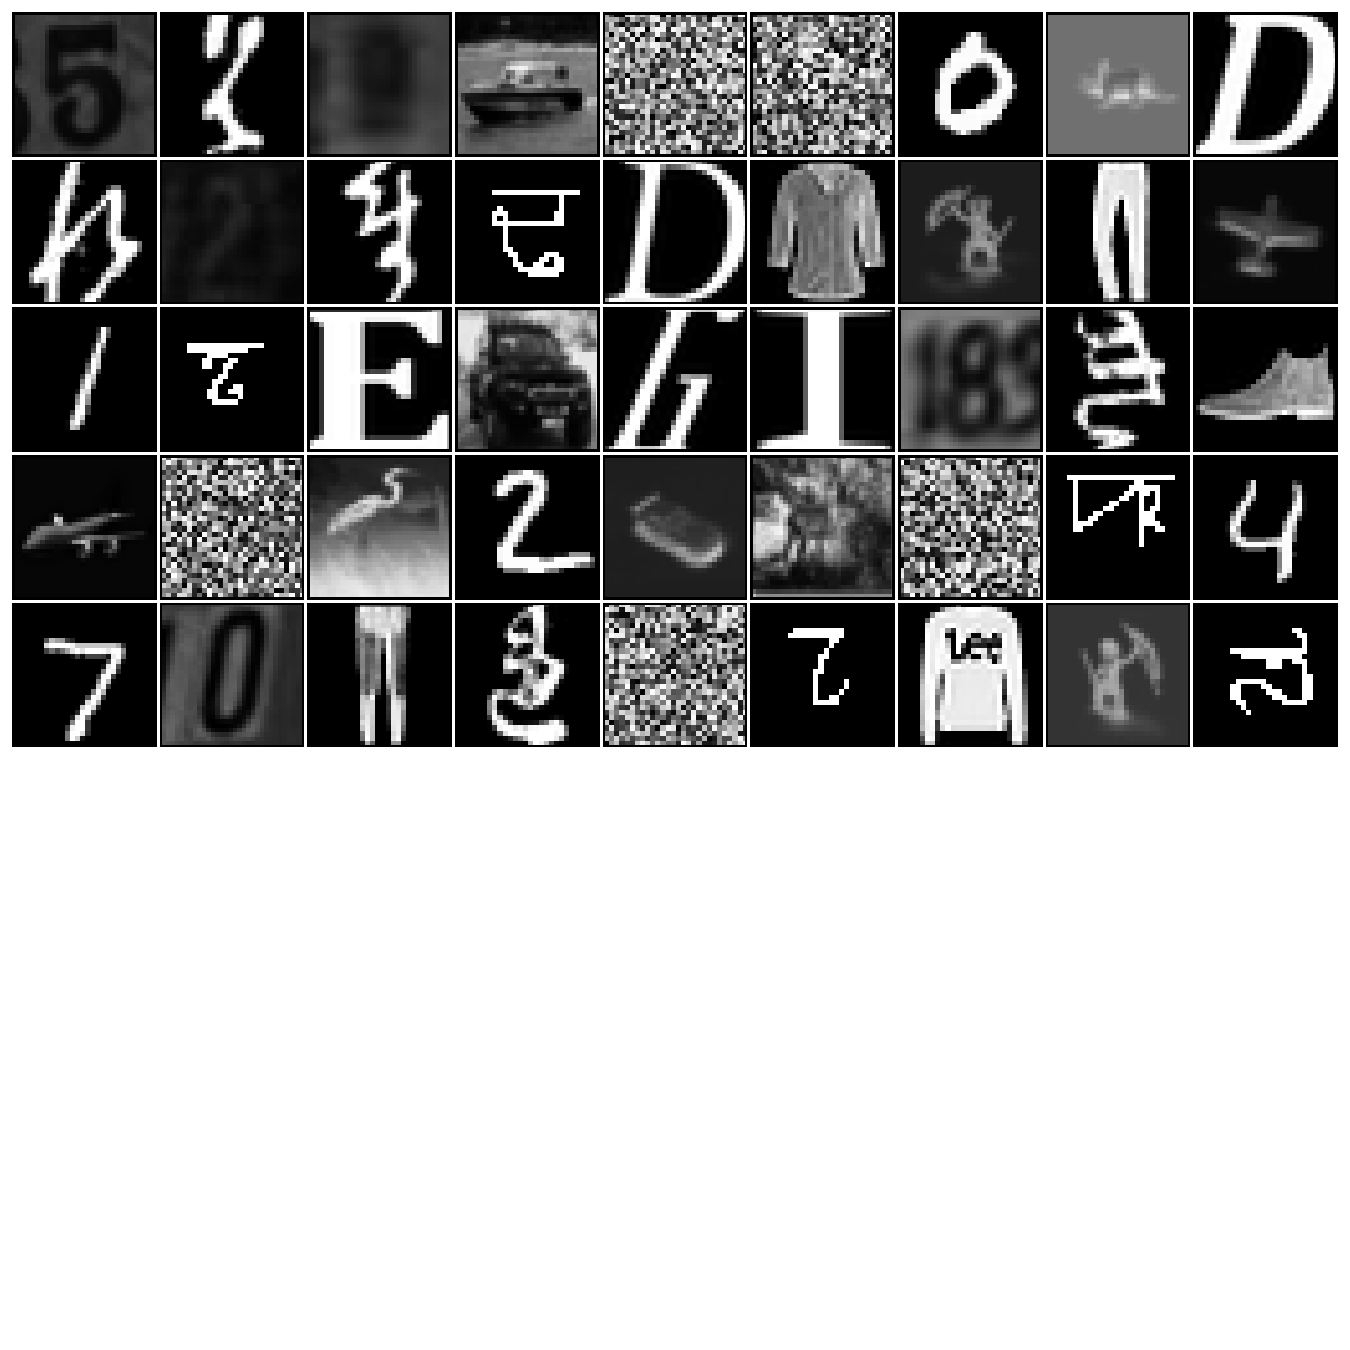
\includegraphics[scale=0.6]{figures/dataexamples_shuffled.pdf}
    \end{figure}
}


\frame{
    \frametitle{Out of distribution?}
    \begin{figure}[\textwidth]
        \centering
        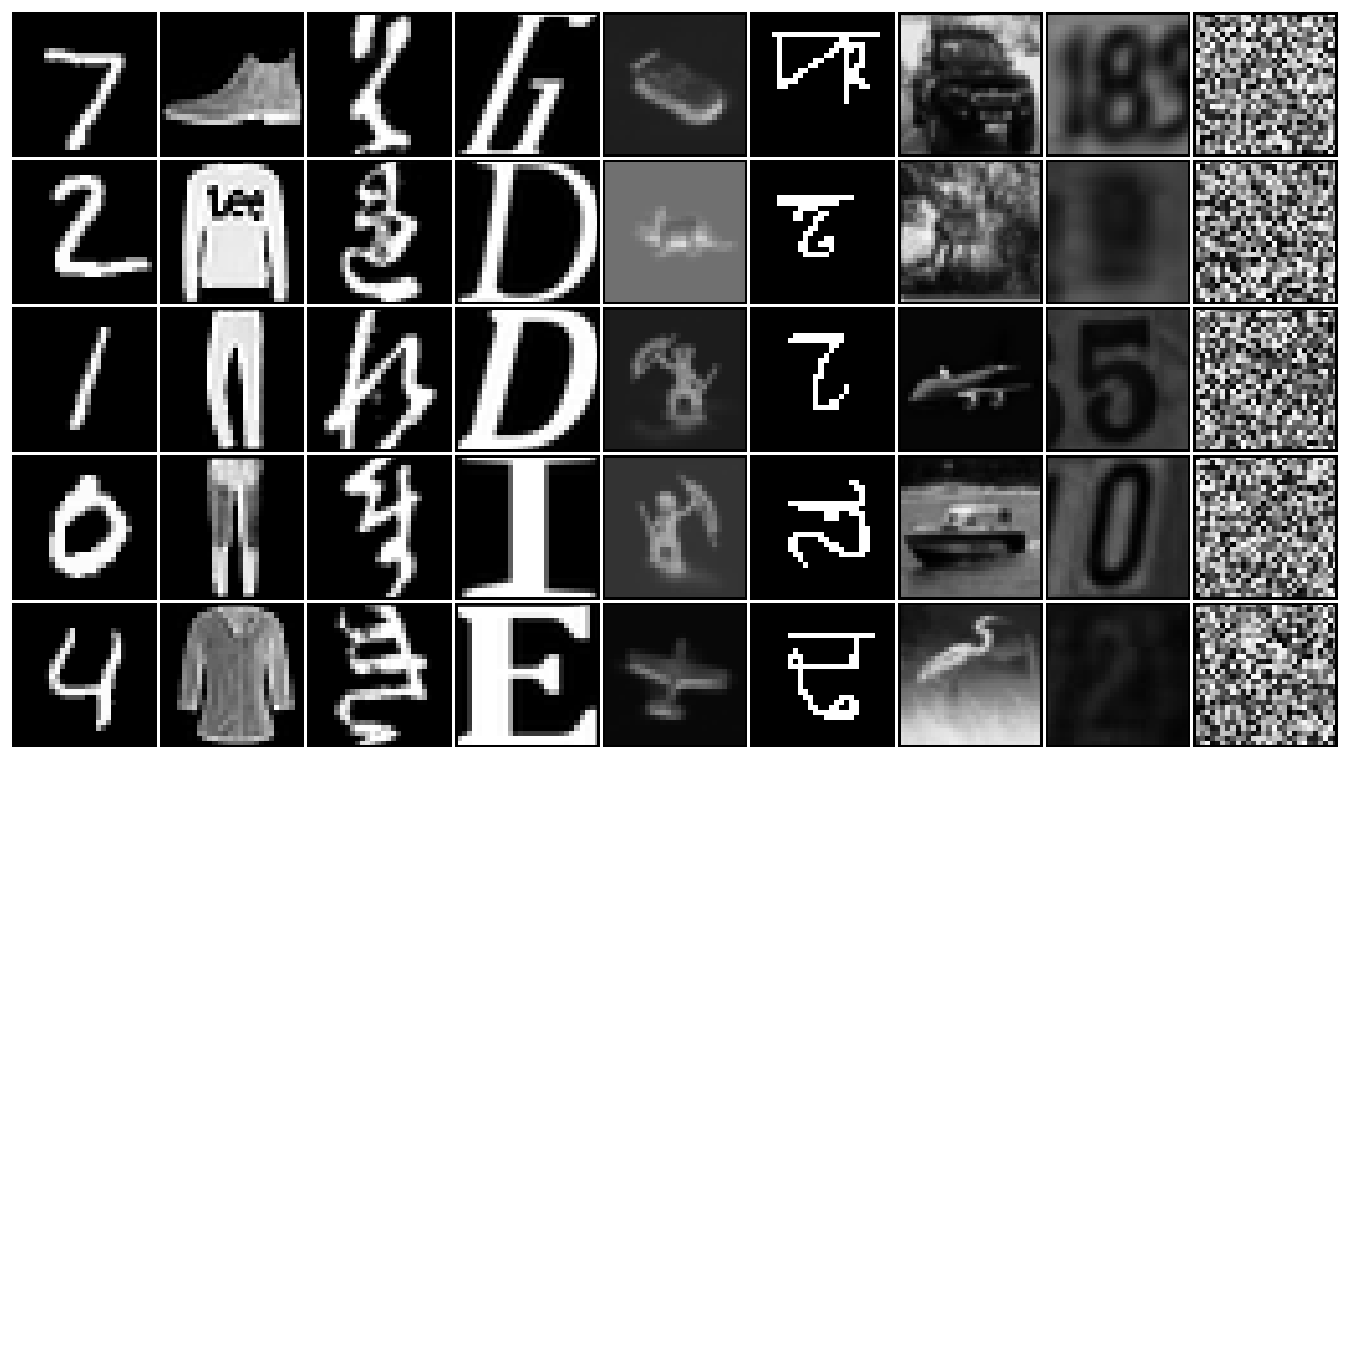
\includegraphics[scale=0.6]{figures/dataexamples.pdf}
    \end{figure}
}



% \section{Latent variable models}

\begin{frame}{Hierarchical VAE}
  \begin{columns}
      \begin{column}{0.7\textwidth}
          We choose the hierarchical VAE as our model \cite{kingma_autoencoding_2014, rezende_stochastic_2014}.
          \begin{equation*}
              p_\theta(\xb) = \int p_\theta(\xb,\zb) \text{d}\zb = \int p_\theta(\xb|\zb)p_\theta(\zb) \text{d}\zb
          \end{equation*}
          Specifically we use
          
          \begin{enumerate}
              \item a three-layered hierarchical VAE with bottom-up inference and deterministic skip-connections for both inference and generation.
              \begin{align*}
                  \text{Generative model: }\quad p_\theta(\xb|\zb) &= p_\theta(\xb|\zb_1) p_\theta(\zb_1|\zb_2) p(\zb_3),\\
                  \text{Inference model: }\quad q_\phi(\zb|\xb) &= q_\phi(\zb_1|\xb)q_\phi(\zb_2|\zb_1)q_\phi(\zb_3|\zb_2).
              \end{align*}
              \item a ten-layered layered Bidirectional-Inference Variational Autoencoder (BIVA) \cite{maaloe_biva_2019}.
          \end{enumerate} 
      \end{column}
      \begin{column}{0.3\textwidth}
          \begin{figure}[.5\textwidth]
          \tikz{
          % inference
          % nodes
          \node[obs] (x_inf) {$\xb$};%
          \node[latent,above=.75cm of x_inf](z1_inf){$\zb_1$}; %
          \node[latent,above=.75cm of z1_inf](z2_inf){$\zb_2$}; %
          \node[latent,above=.75cm of z2_inf](z3_inf){$\zb_3$}; %
          \node[above=of z3_inf, yshift=-1.cm] (phi) {$q_\phi(\zb|\xb)$}; 
          
          % edges
          \edge[]{x_inf}{z1_inf};
          \edge[]{z1_inf}{z2_inf};
          \edge[]{z2_inf}{z3_inf};
          \edge[dashed, bend left]{x_inf}{z2_inf};
          \edge[dashed, bend left]{x_inf}{z3_inf};
          
          % generative
          % nodes$
          \node[obs,right=0.75cm of x_inf] (x_gen) {$\xb$};%
          \node[latent,above=.75cm of x_gen](z1_gen){$\zb_1$}; %
          \node[latent,above=.75cm of z1_gen](z2_gen){$\zb_2$}; %
          \node[latent,above=.75cm of z2_gen](z3_gen){$\zb_3$}; %
          \node[above=of z3_gen, yshift=-1.cm] (theta) {$p_\theta(\xb,\zb)$}; 
          
          % edges
          \edge[]{z3_gen}{z2_gen};
          \edge[]{z2_gen}{z1_gen};
          \edge[]{z1_gen}{x_gen};
          \edge[dashed, bend left]{z2_gen}{x_gen};
          \edge[dashed, bend left]{z3_gen}{x_gen};
          }
          \end{figure}
      \end{column}
  \end{columns}
\end{frame}


\begin{frame}
    \frametitle{Out-of-distribution detection with hierarchical VAEs}
    \begin{columns}
        \begin{column}{0.4\textwidth}
            \begin{itemize}
                \item Generative models learn to approximate the \textbf{data distribution} $p(\xb)$.
                \item The likelihood of the model given a sample $\xb$ is a measure of how well the model \textbf{explains the data}.
                \item \textbf{Model likelihood} has long been thought of as useful for OOD detection \cite{bishop_novelty_1994}.
            \end{itemize}
        \end{column}
        \begin{column}{0.6\textwidth}
            \begin{overprint}
                \onslide<2>
                \begin{figure}
                    \centering
                    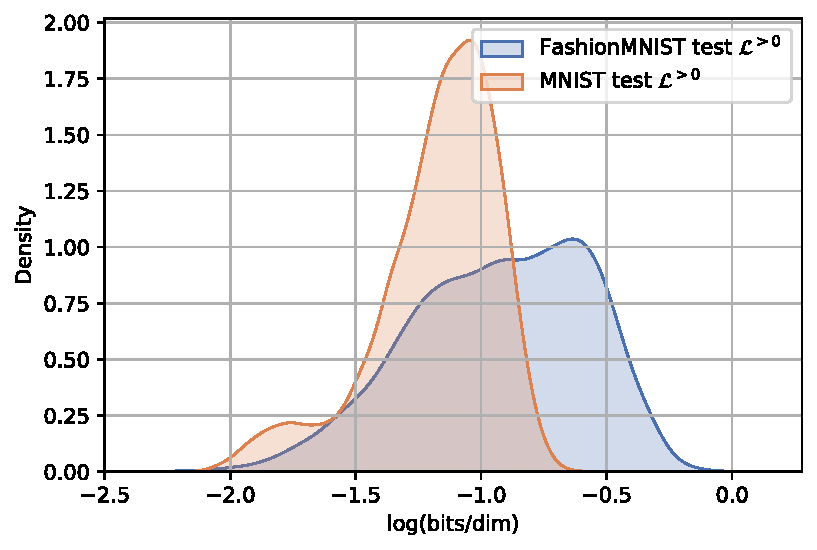
\includegraphics[width=\textwidth]{../graphics/paper_hierarchical/densities-FashionMNIST-test-MNIST-test-bpp-k-0_sohau.pdf}
                \end{figure}
            \end{overprint}
        \end{column}
    \end{columns}
\end{frame}


% \section{Identifying the issue}


\frame{
    \frametitle{What is wrong with the ELBO for OOD detection?}
    We can split the ELBO into two terms
    \begin{equation}
        \mathcal{L}(\xb;\theta,\phi) 
        = \mathbb{E}_{q_\phi(\zb|\xb)} \left[ \log \frac{p_\theta(\xb,\zb)}{q_\phi(\zb|\xb)} \right] 
        = \underbrace{\mathbb{E}_{q_\phi(\zb|\xb)}[\log p_\theta(\xb|\zb)]}_{\text{reconstruction likelihood}} - \underbrace{D_{\mathrm{KL}}( q_\phi(\zb|\xb) || p(\zb))}_{\text{regularization penalty}} \ .
    \end{equation}
    The first term is high if the data is well-explained by $\zb$.

    \vspace{3mm}
    The second term we can rewrite as,
    \begin{equation}
        D_{\mathrm{KL}}( q_\phi(\zb|\xb) || p(\zb)) = \mathbb{E}_{q_\phi(\zb|\xb)} \Big[ \textstyle\sum_{i=1}^{L-1} \log \frac{p_\theta(\zb_i|\zb_{i+1})}{q_\phi(\zb_i|\zb_{i-1})} + \log \frac{p_\theta(\zb_L)}{q_\phi(\zb_L|\zb_{L-1})} \Big] \ .
    \end{equation}
    The absolute log-ratios grow with $\mathrm{dim}(\zb_i)$ since the log probability terms are computed by summing over the dimensionality of $\zb_i$.
    
    \vspace{3mm}
}


\frame{
    \frametitle{What do the lowest latent variables code for?}
    
    Absolute Pearson correlations between data representations in all layers of the inference network of a hierarchical VAE trained on FashionMNIST and of another trained on MNIST. 
    \vspace{0.3cm}

    Correlation computed between the representations of the two different models given the same data, FashionMNIST (top) and MNIST (bottom).
    
    \begin{figure}[\textwidth]
        \centering
        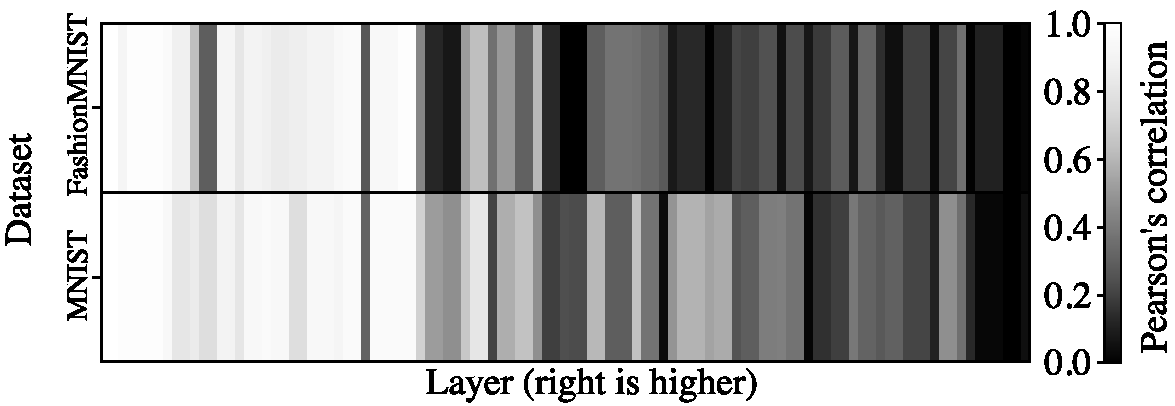
\includegraphics[scale=0.75]{../graphics/paper_hierarchical/feature-correlation-heatmap2.pdf}
        % \caption{Caption}
        % \label{fig:my_label}
    \end{figure}
}


\section{The $\mathcal{L}^{>k}$ likelihood bound}


\frame{
    \frametitle{An alternative likelihood bound, $\mathcal{L}^{>k}$}
    An alternative version of the ELBO that only partially uses the approximate posterior can be written as \cite{maaloe_biva_2019}
    \begin{equation}
        \mathcal{L}^{>k}(\xb; \theta, \phi) = \mathbb{E}_{p_\theta(\zb_{\leq k}|\zb{>k})q_\phi(\zb_{>k}|\xb)} \left[ \log \frac{p_\theta(\xb|\zb)p_\theta(\zb_{>k})}{q_\phi(\zb_{>k}|\xb)} \right]
    \end{equation}
    
    Here, we have replaced the approximate posterior $q_\phi(\zb|\xb)$ with a different proposal distribution that combines part of the approximate posterior with the conditional prior, namely
    
    $$p_\theta(\zb_{\leq k}|\zb_{>k})q_\phi(\zb_{>k}|\xb)$$
    
    This bound uses the conditional prior for the lowest latent variables in the hierarchy.
}


\section{Likelihood ratio}


\frame{
    \frametitle{Likelihood ratios}
    We can use our new bound to compute the score used in a standard likelihood ratio test \cite{buse_likelihood_1982}.
    \begin{equation}\label{eq:llr-as-difference-in-likelihoods}
        LLR^{>k}(\xb) \equiv \mathcal{L}(\xb) - \mathcal{L}^{>k}(\xb) \ .
    \end{equation}
    We can inspect what this likelihood-ratio measures by considering the exact form of our bounds.
    \begin{align}
        \mathcal{L}      &= \log p_\theta(\xb) - D_{\mathrm{KL}}\left( q_\phi(\zb|\xb) || p_\theta(\zb|\xb)\right), \label{eq:likelihoods-as-exact} \\ 
        \mathcal{L}^{>k} &= \log p_\theta(\xb) - D_{\mathrm{KL}}\left( p_\theta(\zb_{\leq }|\zb_{>k}) q_\phi(\zb_{>k}|\xb) || p_\theta(\zb|\xb)\right) \notag \ .
    \end{align}
    In the likelihood ratio the reconstruction terms cancel out and only the KL-divergences from the approximate to the true posterior remain.
    \begin{align}\label{eq:llr-as-kls}
        LLR^{>k}(\xb) &= - D_{\mathrm{KL}}\left( q_\phi(\zb|\xb) || p_\theta(\zb|\xb)\right) \\
                     &\quad + D_{\mathrm{KL}}\left( p_\theta(\zb_{\leq }|\zb_{>k}) q_\phi(\zb_{>k}|\xb) || p_\theta(\zb|\xb)\right) \ . \notag
    \end{align}
}


\frame{
    \frametitle{Importance sampling the ELBO}
    The importance weighted autoencoder (IWAE) bound is tight with the true likelihood in the limit of infinite samples, $S\rightarrow\infty$ \cite{burda_importance_2016},
    \begin{equation}\label{eq:iw-bound}
        \mathcal{L}_{S} = \mathbb{E}_{q(\zb|\xb)}\left[ \log \frac{1}{N} \sum_{s=1}^{S} \frac{p(\xb, \zb^{(s)})}{q(\zb^{(s)}|\xb)} \right] \leq \log p_\theta(\xb) \ ,
    \end{equation}

    \vspace{3mm}

    Consequently, by importance sampling the ELBO, the associated KL-divergence vanishes and our likelihood ratio reduces to the KL-divergence of $\mathcal{L}^{>k}$.

    \begin{equation}\label{eq:llr-as-kls-iwae-reduced}
        LLR^{>k}_{S}(\xb) \rightarrow D_{\mathrm{KL}}( p(\zb_{\leq }|\zb_{>k}) q(\zb_{>k}|\xb) || p(\zb|\xb)) \ .
    \end{equation}

    $LLR^{>k}_{S}(\xb)$ performs KL-divergence-based OOD detection using top-most latent variables.
}


\frame{
    \frametitle{Results with $LLR^{>k}$}
    \begin{figure}[\textwidth]
    \centering
    \begin{subfigure}[c]{0.49\textwidth}
        \centering
        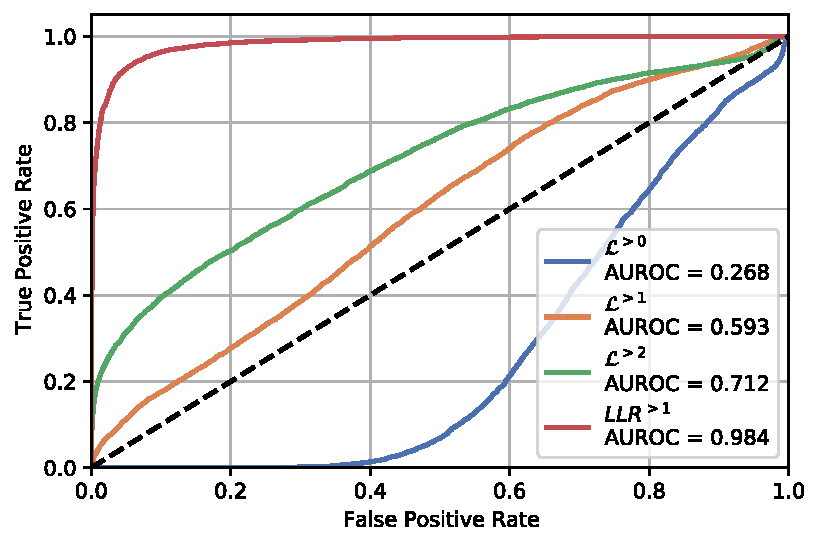
\includegraphics[width=\textwidth]{../graphics/paper_hierarchical/roc-FashionMNIST-test-MNIST-test-ll-and-llr-IW250_sohau.pdf}
        \caption{FashionMNIST HVAE evaluated on MNIST}
    \end{subfigure}
    \hfill
    \begin{subfigure}[c]{0.49\textwidth}
        \centering
        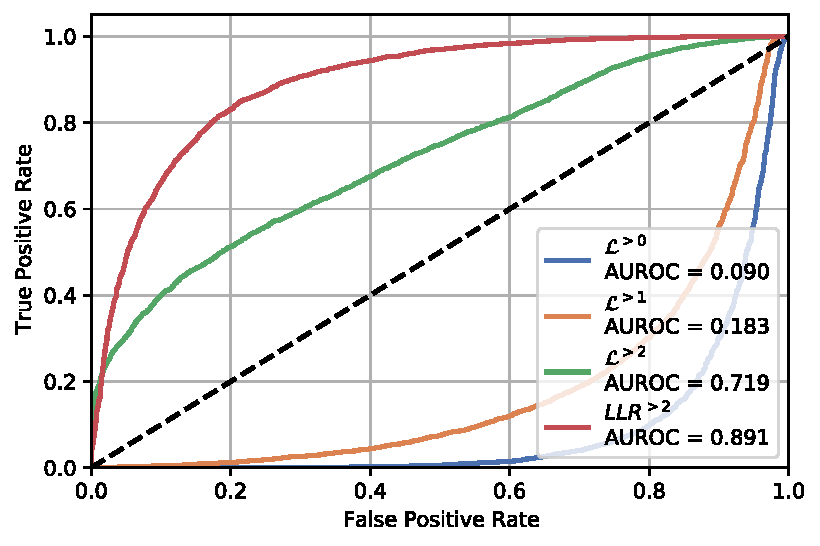
\includegraphics[width=\textwidth]{../graphics/paper_hierarchical/roc-biva-CIFAR10-SVHN-ll-and-llr_sohau.pdf}
        \caption{CIFAR10 BIVA evaluated on SVHN}
    \end{subfigure}
    \end{figure}
}


\begin{frame}
    \frametitle{Results on FashionMNIST/MNIST}
    \begin{table}
        \centering
        \resizebox*{!}{0.87\textheight}{%
        \begin{tabular}{lrrr}
            \toprule
            Method & AUROC$\uparrow$ & AUPRC$\uparrow$ & FPR80$\downarrow$ \\
            \midrule
            \multicolumn{4}{c}{\textbf{FashionMNIST (in) / MNIST (out)}} \\
            \midrule
            \multicolumn{4}{l}{\textbf{Use prior knowledge of OOD}} \\
            Backgr. contrast. LR (PixelCNN) {\parencite{ren_likelihood_2019}}               & $0.994$ & $0.993$ & $0.001$ \\
            Backgr. contrast. LR (VAE) {\parencite{choi_waic_2019}}                    & $0.924$ & - & - \\
            Binary classifier {\parencite{ren_likelihood_2019}}                              & $0.455$ & $0.505$ & $0.886$ \\ % 6
            $p(\hat{y} | \xb)$ with OOD as noise class {\parencite{ren_likelihood_2019}}     & $0.877$ & $0.871$ & $0.195$ \\ % 7
            $p(\hat{y} | \xb)$ with calibration on OOD {\parencite{ren_likelihood_2019}}     & $0.904$ & $0.895$ & $0.139$ \\ % 8
            Input complexity ($S$, Glow) \parencite{hendrycks_deep_2019}                    & $0.998$ & - & - \\
            Input complexity ($S$, PixelCNN++) \parencite{hendrycks_deep_2019}              & $0.967$ & - & - \\
            \multicolumn{4}{l}{\textbf{Use in-distribution data labels $y$}} \\
            $p(\hat{y} | \xb)$ {\parencite{ren_likelihood_2019, hendrycks_baseline_2017}}                        & $0.734$ & $0.702$ & $0.506$ \\
            Entropy of $p(y | \xb)$ {\parencite{ren_likelihood_2019}}                        & $0.746$ & $0.726$ & $0.448$ \\
            ODIN {\parencite{ren_likelihood_2019, liang_enhancing_2018}}                                       & $0.752$ & $0.763$ & $0.432$ \\
            VIB \parencite{alemi_uncertainty_2018, choi_waic_2019}                                          & $0.941$ & - & - \\
            Mahalanobis distance, CNN {\parencite{ren_likelihood_2019}}                     & $0.942$ & $0.928$ & $0.088$ \\
            Mahalanobis distance, DenseNet {\parencite{lee_simple_2018}}                & $0.986$ & - & - \\
            Ensemble, 20 classifiers {\parencite{ren_likelihood_2019, lakshminarayanan_simple_2017}}                  & $0.857$ & $0.849$ & $0.240$ \\
            \multicolumn{4}{l}{\textbf{No OOD-specific assumptions}} \\
            \multicolumn{4}{l}{\textit{- Ensembles}} \\
            WAIC, 5 models, VAE {\parencite{choi_waic_2019}}                          & $0.766$ & - & - \\
            WAIC, 5 models, PixelCNN {\parencite{ren_likelihood_2019}}                      & $0.221$ & $0.401$ & $0.911$ \\
            \multicolumn{4}{l}{\textit{- Not ensembles}} \\
            Likelihood regret \parencite{xiao_likelihood_2020}                               & $\mathbf{0.988}$ & - & - \\
            $\mathcal{L}^{>0}$ + HVAE (ours)                    & $0.268$ & $0.363$ & $0.882$ \\
            $\mathcal{L}^{>1}$ + HVAE (ours)                    & $0.593$ & $0.591$ & $0.658$ \\
            $\mathcal{L}^{>2}$ + HVAE (ours)                    & $0.712$ & $0.750$ & $0.548$ \\
            $LLR^{>1}$ + HVAE (ours)                            & $0.964$ & $0.961$ & $0.036$ \\
            $LLR^{>1}_{250}$ + HVAE (ours)                      & $0.984$ & $\mathbf{0.984}$ & $\mathbf{0.013}$ \\
             \bottomrule
        \end{tabular}%
        }
    \end{table}
\end{frame}


\begin{frame}
    \frametitle{Results on CIFAR10/SVHN}
    \begin{table}
        \centering
        \resizebox*{!}{0.87\textheight}{%
        \begin{tabular}{lrrr}
            \toprule
            Method & AUROC$\uparrow$ & AUPRC$\uparrow$ & FPR80$\downarrow$ \\
            \midrule
            \multicolumn{4}{c}{\textbf{CIFAR10 (in) / SVHN (out)}} \\
            \midrule
            \multicolumn{4}{l}{\textbf{Use prior knowledge of OOD}} \\
            Backgr. contrast. LR (PixelCNN) {\parencite{ren_likelihood_2019}}               & $0.930$ & $0.881$ & $0.066$ \\
            Backgr. contrast. LR (VAE) {\parencite{xiao_likelihood_2020}}                    & $0.265$ & - & - \\
            Outlier exposure {\parencite{hendrycks_deep_2019}}                              & $0.984$ & - & - \\
            Input complexity ($S$, Glow) \parencite{serra_input_2020}                   & $0.950$ & - & - \\
            Input complexity ($S$, PixelCNN++) \parencite{serra_input_2020}             & $0.929$ & - & - \\
            Input complexity ($S$, HVAE) (Ours) \parencite{serra_input_2020} & $0.833$ & $0.855$ & $0.344$ \\
            \multicolumn{4}{l}{\textbf{Use in-distribution data labels $y$}} \\
            Mahalanobis distance {\parencite{lee_simple_2018}}                          & $0.991$ & - & -  \\
            \multicolumn{4}{l}{\textbf{No OOD-specific assumptions}} \\
            \multicolumn{4}{l}{\textit{- Ensembles}} \\
            WAIC, 5 models, Glow {\parencite{choi_waic_2019}}                          & $1.000$ & - & - \\
            WAIC, 5 models, PixelCNN {\parencite{ren_likelihood_2019}}                      & $0.628$ & $0.616$ & $0.657$ \\
            \multicolumn{4}{l}{\textit{- Not ensembles}} \\
            Likelihood regret \parencite{xiao_likelihood_2020}                               & $0.875$ & - & - \\
            $LLR^{>2}$ + HVAE (ours)                            & $0.811$ & $0.837$ & $0.394$ \\
            $LLR^{>2}$ + BIVA (ours)                            & $\mathbf{0.891}$ & $\mathbf{0.875}$ & $\mathbf{0.172}$ \\
            \bottomrule
        \end{tabular}%
        }
    \end{table}
\end{frame}



\frame{
    \frametitle{Results on diverse datasets}
    \begin{columns}
        \begin{column}{0.5\textwidth}
            \begin{table}[t]
                \centering
                \resizebox{0.9\textwidth}{!}{%
                \begin{tabular}{llrrr}
                    \toprule
                    OOD dataset & Metric & AUROC$\uparrow$ & AUPRC$\uparrow$ & FPR80$\downarrow$ \\
                    \midrule
                    \multicolumn{5}{c}{\textbf{Trained on CIFAR10}} \\
                    \midrule
                    SVHN          &  $LLR^{>2}$  &  0.811  &  0.837  &  0.394  \\
                    CIFAR10       &  $LLR^{>1}$  &  0.469  &  0.479  &  0.835  \\
                    \midrule
                    \multicolumn{5}{c}{\textbf{Trained on SVHN}} \\
                    \midrule
                    CIFAR10            &  $LLR^{>1}$       &  $0.939$  &  $0.950$  &  $0.052$  \\
                    SVHN               &  $LLR^{>1}$       &  $0.489$  &  $0.484$  &  $0.799$  \\
                    \bottomrule
                \end{tabular}
                }
            \end{table}
        \end{column}
        \begin{column}{0.5\textwidth}
            \begin{table}[t]
                \centering
                \resizebox{0.9\textwidth}{!}{%
                \begin{tabular}{llrrr}
                    \toprule
                    OOD dataset & Metric & AUROC$\uparrow$ & AUPRC$\uparrow$ & FPR80$\downarrow$ \\
                    \midrule
                    \multicolumn{5}{c}{\textbf{Trained on FashionMNIST}} \\
                    \midrule
                    MNIST                    & $LLR^{>1}$             &  0.986  &  0.987  &  0.011 \\
                    notMNIST                 &  $LLR^{>1}$            &  0.998  &  0.998  &  0.000 \\
                    KMNIST                   &  $LLR^{>1}$            &  0.974  &  0.977  &  0.017 \\
                    Omniglot28x28            &  $LLR^{>2}$            &  1.000  &  1.000  &  0.000 \\
                    Omniglot28x28Inverted    &  $LLR^{>1}$            &  0.954  &  0.954  &  0.050 \\
                    SmallNORB28x28           &  $LLR^{>2}$            &  0.999  &  0.999  &  0.002 \\
                    SmallNORB28x28Inverted   &  $LLR^{>2}$            &  0.941  &  0.946  &  0.069 \\
                    FashionMNIST             &  $LLR^{>1}$            &  0.488  &  0.496  &  0.811 \\
                    \midrule
                    \multicolumn{5}{c}{\textbf{Trained on MNIST}} \\
                    \midrule
                    FashionMNIST                   &  $LLR^{>1}$  &  $0.999$  &  $0.999$  &  $0.000$ \\
                    notMNIST                       &  $LLR^{>1}$  &  $1.000$  &  $0.999$  &  $0.000$ \\
                    KMNIST                         &  $LLR^{>1}$  &  $0.999$  &  $0.999$  &  $0.000$ \\
                    Omniglot28x28                  &  $LLR^{>1}$  &  $1.000$  &  $1.000$  &  $0.000$ \\
                    Omniglot28x28Inverted          &  $LLR^{>1}$  &  $0.944$  &  $0.953$  &  $0.057$ \\
                    SmallNORB28x28                 &  $LLR^{>1}$  &  $1.000$  &  $1.000$  &  $0.000$ \\
                    SmallNORB28x28Inverted         &  $LLR^{>1}$  &  $0.985$  &  $0.987$  &  $0.000$ \\
                    MNIST                          &  $LLR^{>2}$  &  $0.515$  &  $0.507$  &  $0.792$ \\
                    \bottomrule
                \end{tabular}
                }
            \end{table}
        \end{column}
    \end{columns}
}


% \frame{
%     \frametitle{Results with $LLR^{>k}$}
%     % The score has good performance across many different datasets.
    
%     \begin{columns}

%     \begin{column}{0.5\textwidth}

%         \begin{table}[t]
%             \centering
%             \resizebox{0.6\textwidth}{!}{%
%             \begin{tabular}{llr}
%                 \toprule
%                  OOD dataset & Metric & AUROC$\uparrow$ \\
%                  \midrule
%                  \multicolumn{3}{c}{\textbf{Trained on CIFAR10}} \\
%                  \midrule
%         SVHN          &  $LLR^{>2}$  &  0.811 \\
%         CIFAR10       &  $LLR^{>1}$  &  0.469 \\
%                  \midrule
%                  \multicolumn{3}{c}{\textbf{Trained on SVHN}} \\
%                  \midrule
%         CIFAR10            &  $LLR^{>1}$       &  0.939 \\
%         SVHN               &  $LLR^{>1}$       &  0.489 \\
%             \bottomrule
%             \end{tabular}
%             }
%         \end{table}
%     \end{column}
    
%     \begin{column}{0.5\textwidth}
%         \begin{table}[t]
%             \centering
%             \resizebox{0.75\textwidth}{!}{%
%             \begin{tabular}{llr}
%                 \toprule
%                  OOD dataset & Metric & AUROC$\uparrow$ \\
%                  \midrule
%                  \multicolumn{3}{c}{\textbf{Trained on FashionMNIST}} \\
%                  \midrule
%         MNIST                    & $LLR^{>1}$             &  0.986 \\
%         notMNIST                 &  $LLR^{>1}$            &  0.998 \\
%         KMNIST                   &  $LLR^{>1}$            &  0.974 \\
%         Omniglot28x28            &  $LLR^{>2}$            &  1.000 \\
%         Omniglot28x28Inverted    &  $LLR^{>1}$            &  0.954 \\
%         SmallNORB28x28           &  $LLR^{>2}$            &  0.999 \\
%         SmallNORB28x28Inverted   &  $LLR^{>2}$            &  0.941 \\
%         FashionMNIST             &  $LLR^{>1}$            &  0.488 \\
%                  \midrule
%                  \multicolumn{3}{c}{\textbf{Trained on MNIST}} \\
%                  \midrule
%         FashionMNIST                   &  $LLR^{>1}$  &  0.999 \\
%         notMNIST                       &  $LLR^{>1}$  &  1.000 \\
%         KMNIST                         &  $LLR^{>1}$  &  0.999 \\
%         Omniglot28x28                  &  $LLR^{>1}$  &  1.000 \\
%         Omniglot28x28Inverted          &  $LLR^{>1}$  &  0.944 \\
%         SmallNORB28x28                 &  $LLR^{>1}$  &  1.000 \\
%         SmallNORB28x28Inverted         &  $LLR^{>1}$  &  0.985 \\
%         MNIST                          &  $LLR^{>2}$  &  0.515 \\
%                  \bottomrule
%             \end{tabular}
%             }
%             % \caption{Additional results for the HVAE model trained on FashionMNIST. All results computed with 1000 importance samples.}
%             % \label{tab:additional-results-fashionmnist}
%         \end{table}
%     \end{column}

%    \end{columns}
%}


\part{Medical Applications}
% !TEX root = ../presentation.tex
% !BIB program = biber
% !TEX program = xelatex

\begin{frame}
    \frametitle{Outline of \partname}
    \tableofcontents
\end{frame}

% !TEX root = ../presentation.tex
% !BIB program = biber
% !TEX program = xelatex

\section[A Retrospective Study on Machine Learning-Assisted Stroke Recognition for Medical Helpline Calls]{A Retrospective Study on Machine Learning-Assisted Stroke Recognition\\ for Medical Helpline Calls}


\begin{frame}
    \frametitle{Stroke}
    \begin{itemize}
        \item Stroke is a leading cause of {\color{dtured}disability and death} worldwide \parencite{cite1,cite2,cite3}.
        \item Effective treatment is very {\color{dtured}time-sensitive}. \parencite{cite4,cite5}.
        \item The gateway to {\color{dtured}ambulance transport and hospital admittance} is through {\color{dtured}prehospital telehealth services}.
        \item {\color{dtured}Mobile stroke units} has made it possible to deliver advanced treatment faster \parencite{cite6,cite7}.
        \item The effectiveness of mobile stroke units hinges on {\color{dtured}call-taker recognition of stroke} \parencite{cite6,cite7}.
        \item But stroke 
    \end{itemize}
\end{frame}


\begin{frame}
    \frametitle{The study}
    \begin{itemize}
        \item Collaboration between {\color{dtured}Corti} and the {\color{dtured}Copenhagen Emergency Medical Services (CEMS)} (``Akutberedskabet").
        \item CEMS provides prehospital telehealth services in the Capital Region of Denmark (1.9M people).
        \item CEMS operates the 1-1-2 emergency line (similar to 9-1-1) and the 1813 medical helpline (non-life-threatening conditions when general practitioner is unavailable).
        \item Approximately half of all patients with stroke do not receive the correct triage for their condition from call-takers \parencite{cite10,cite11,cite12}. 
        \vspace{1em}
        \item We wanted to investigate if a machine learning model could assist call-takers of 1813 in recognizing stroke.
    \end{itemize}
\end{frame}


\begin{frame}
    \frametitle{Population selection and datasets}
    \begin{figure}
        \centering
        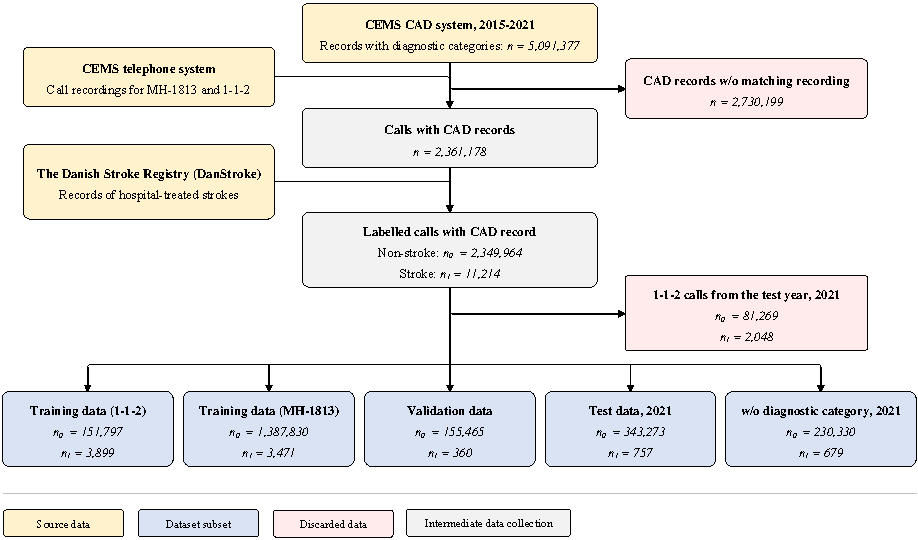
\includegraphics[width=0.65\paperwidth]{../graphics/paper_retrospective/data_flowchart.pdf}
        % \caption{Overview of data flow from the initial data sources to the final stroke dataset.}
    \end{figure}
\end{frame}


\begin{frame}
    \frametitle{Population characteristics}
    \begin{table}[t]
        \centering
        % \caption{Population characteristics for each data subset.}
        % \label{tab_retrospective:table1-population-characteristics}
        \resizebox*{0.98\textwidth}{!}{%
        \begin{tabular}{l|ccccc}
            \toprule
                                  & Training (112) & Training (MH-1813) & Validation & Test & 2021 w/o category \\
    
            \midrule
            \multicolumn{6}{c}{\emph{All calls}} \\
            \midrule
            Num. calls            & 155,696 & 1,391,301 & 155,825 & 344,030 & 231,009 \\
            Female                & 74,640 (47.94\%) & 792,783 (56.98\%) & 86,959 (55.81\%) & 190,974 (55.51\%) & 134,324 (58.14\%) \\
            Male                  & 79,564 (51.10\%) & 596,760 (42.89\%) & 68,866 (44.19\%) & 153,050 (44.49\%) & 96,258 (41.67\%) \\
            65+ years             & 72,930 (46.84\%) & 335,146 (24.09\%) & 30,313 (19.45\%) & 65,652 (19.08\%) & 81,488 (35.27\%) \\
            Age (mean $\pm$ std.) & 59.47 ± 21.24 & 47.12 ± 21.38 & 44.63 ± 20.08 & 44.31 ± 20.10 & 50.36 ± 22.77 \\
    
            \midrule
            \multicolumn{6}{c}{\emph{Stroke calls}} \\
            \midrule
            Num. calls            & 3,899 & 3,471 & 360 & 757 & 679 \\
            Female                & 1,784 (45.76\%) & 1,654 (47.65\%) & 161 (44.72\%) & 349 (46.10\%) & 366 (53.90\%) \\
            Male                  & 2,115 (54.24\%) & 1,815 (52.29\%) & 199 (55.28\%) & 408 (53.90\%) & 313 (46.10\%) \\
            65+ years             & 2,968 (76.12\%) & 2,421 (69.75\%) & 250 (69.44\%) & 555 (73.32\%) & 567 (83.51\%) \\
            Age (mean $\pm$ std.) & 72.91 ± 12.77 & 70.68 ± 13.85 & 70.93 ± 13.83 & 71.51 ± 13.41 & 73.41 ± 14.11 \\
    
            \midrule
            \multicolumn{6}{c}{\emph{Non-stroke calls}} \\
            \midrule
            Num. calls            & 151,797 & 1,387,830 & 155,465 & 343,273 & 230,330 \\
            Female                & 72,856 (48.00\%) & 791,129 (57.00\%) & 86,798 (55.83\%) & 190,625 (55.53\%) & 133,958 (58.16\%) \\
            Male                  & 77,449 (51.02\%) & 594,945 (42.87\%) & 68,667 (44.17\%) & 152,642 (44.47\%) & 95,945 (41.66\%) \\
            65+ years             & 69,962 (46.09\%) & 332,725 (23.97\%) & 30,063 (19.34\%) & 65,097 (18.96\%) & 80,921 (35.13\%) \\
            Age (mean $\pm$ std.) & 59.12 ± 21.30 & 47.06 ± 21.36 & 44.57 ± 20.05 & 44.25 ± 20.08 & 50.29 ± 22.76 \\
    
            \bottomrule
        \end{tabular}%
        }
    \end{table}
    % \begin{figure}
    %     \centering
    %     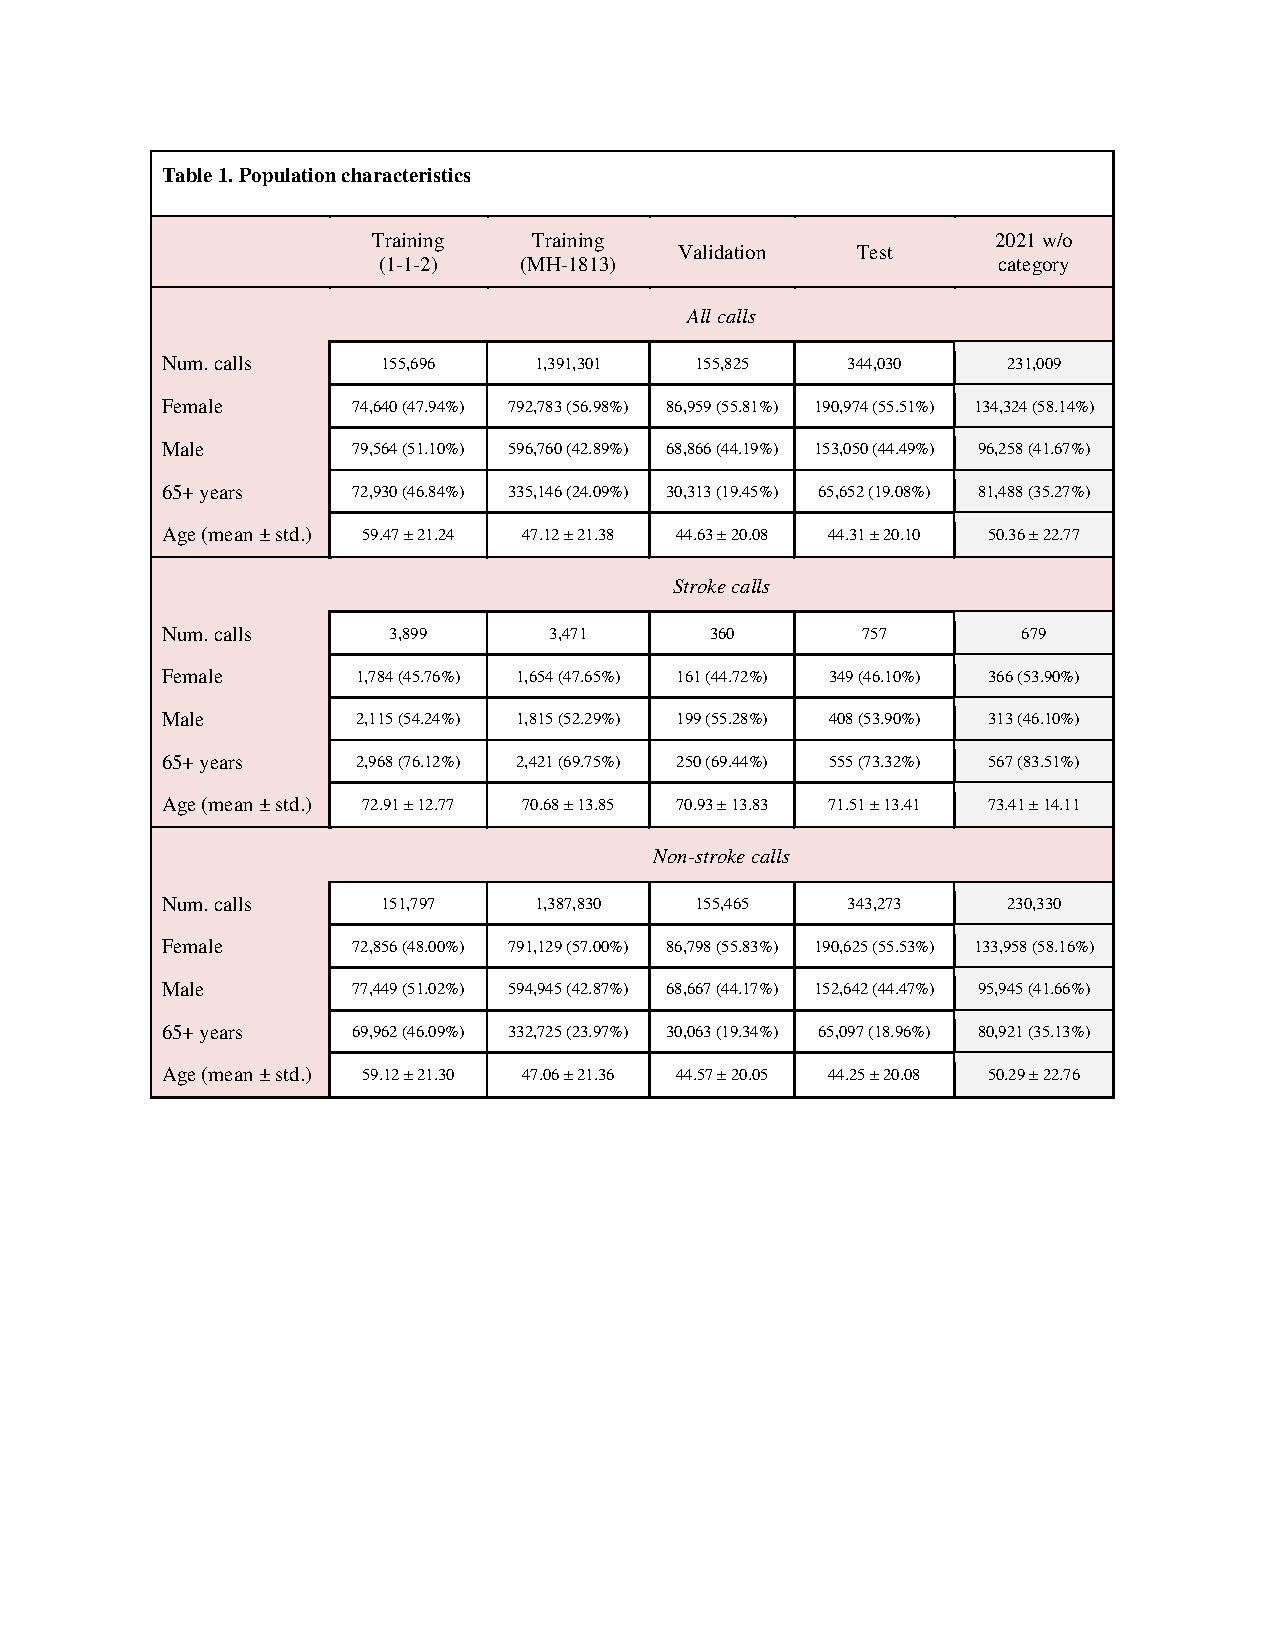
\includegraphics[width=0.45\paperwidth]{../graphics/paper_retrospective/table1.pdf}
    % \end{figure}
\end{frame}


\begin{frame}
    \frametitle{Model design}
    \begin{figure}
        \centering
        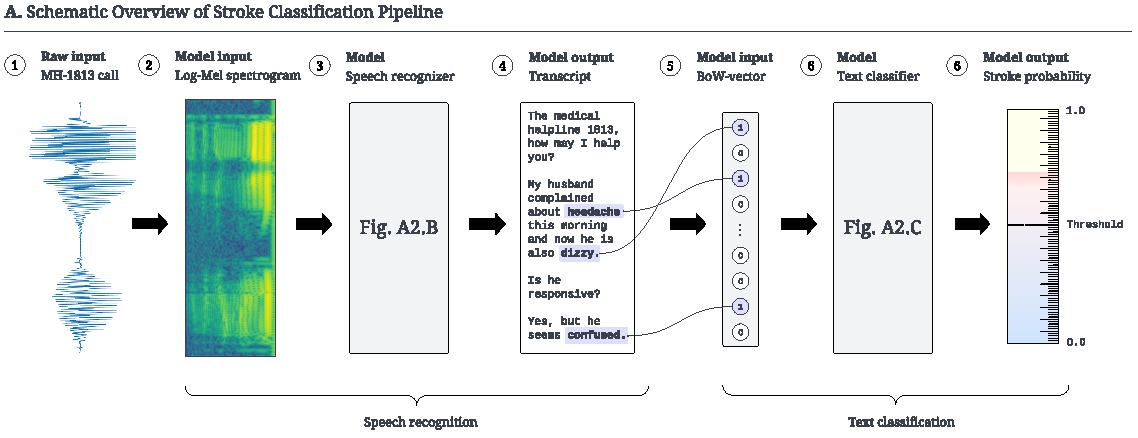
\includegraphics[width=0.90\paperwidth]{../graphics/paper_retrospective/model_sketch-top-part.pdf}
    \end{figure}
\end{frame}


\begin{frame}
    \frametitle{Model design}
    \begin{figure}
        \centering
        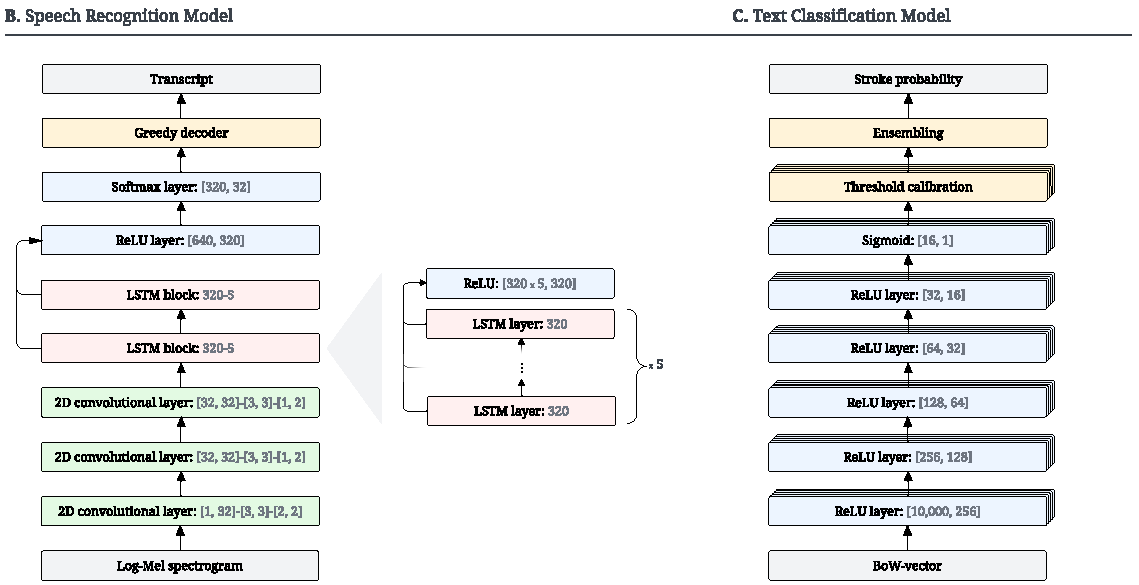
\includegraphics[width=0.70\paperwidth]{../graphics/paper_retrospective/model_sketch-bottom-part.pdf}
    \end{figure}
\end{frame}


\begin{frame}
    \frametitle{Main results}
    \begin{table}[t]
        \centering
        \caption[Overall stroke recognition performance of model compared to call-takers.]{Overall performance on MH-1813 test data, performance without 1-1-2 training data, and performance on data from 2021 without diagnostic categories as well as performance on MH-1813 based on demographic subgroups (age/sex) [mean (95\% CI)]. NPV: negative predictive value, PPV: positive predictive value, FOR: false omission rate, CI: confidence interval.}
        \label{tab_retrospective:table2-main-results}
        \resizebox*{0.98\textwidth}{!}{%
        \begin{tabular}{l|ccccc}
            \toprule
                        & F1-score [\%] $\uparrow$ & Sensitivity [\%] $\uparrow$ & PPV [\%] $\uparrow$ & \makecell{FOR [\%] $\downarrow$ \\ (1 - specificity)} & \makecell{FPR [\%] $\downarrow$ \\ (1 - NPV)} \\
    
            \midrule
            \multicolumn{6}{c}{\emph{Overall}} \\
            \midrule
            Call-takers                                 & 25.8 (23.7-27.9) & 52.7 (49.2-56.4) & 17.1 (15.5-18.6) & 0.105 (0.094-0.116) & 0.565 (0.539-0.590) \\
            Model                                       & 35.7 (35.0-36.4) & 63.0 (62.0-64.1) & 24.9 (24.3-25.5) & 0.082 (0.079-0.085) & 0.419 (0.413-0.426) \\
            % \makecell[l]{Model \\ w/o 1-1-2 training data} & 32.4 (31.8-33.1) & 60.4 (59.3-61.4) & 22.2 (21.6-22.7) & 0.088 (0.085-0.091) & 0.467 (0.460-0.474) \\
            % \midrule
    
            \midrule
            \multicolumn{6}{c}{\emph{Without 112 training data}} \\
            \midrule
            Model       & 32.4 (31.8-33.1) & 60.4 (59.3-61.4) & 22.2 (21.6-22.7) & 0.088 (0.085-0.091) & 0.467 (0.460-0.474) \\
    
            \midrule
            \multicolumn{6}{c}{\emph{On MH-1813 data without diagnostic category}} \\
            \midrule
            Model                                       & 32.6 (31.9-33.4) & 48.3 (47.2-49.4) & 24.7 (23.9-25.3) & 0.153 (0.148-0.158) & 0.435 (0.427-0.443) \\
    
            \midrule
            \multicolumn{6}{c}{\emph{18-64 years}} \\
            \midrule
            Call-takers                                 & 15.9 (13.1-18.5) & 50.5 (43.6-57.2) & 9.40 (7.61-11.18) & 0.036 (0.028-0.043) & 0.353 (0.331-0.375) \\
            Model                                       & 22.9 (21.8-24.0) & 54.1 (52.1-56.3) & 14.5 (13.8-15.3) & 0.033 (0.031-0.035) & 0.231 (0.226-0.236) \\ 
    
            \midrule
            \multicolumn{6}{c}{\emph{65+ years}} \\
            \midrule
            Call-takers                                 & 32.9 (30.1-35.7) & 53.5 (49.4-57.6) & 23.7 (21.4-26.0) & 0.401 (0.352-0.449) & 1.467 (1.373-1.560) \\
            Model                                       & 42.8 (41.9-43.7) & 66.3 (65.1-67.5) & 31.6 (30.8-32.4) & 0.290 (0.278-0.303) & 1.224 (1.198-1.249) \\
    
            \midrule
            \multicolumn{6}{c}{\emph{Male}} \\
            \midrule
            Call-takers                                 & 30.2 (27.2-33.3) & 53.9 (49.1-58.9) & 21.0 (18.5-23.5) & 0.124 (0.105-0.141) & 0.542 (0.506-0.580) \\
            Model                                       & 39.0 (38.0-40.1) & 63.7 (62.3-65.2) & 28.1 (27.3-29.0) & 0.097 (0.093-0.102) & 0.435 (0.425-0.445) \\
    
            \midrule
            \multicolumn{6}{c}{\emph{Female}} \\
            \midrule
            Call-takers                                 & 21.9 (19.1-24.6) & 51.3 (46.0-56.6) & 13.9 (12.0-15.8) & 0.090 (0.076-0.103) & 0.582 (0.547-0.616) \\
            Model                                       & 32.4 (31.4-33.4) & 62.3 (60.7-63.8) & 21.9 (21.1-22.7) & 0.069 (0.066-0.073) & 0.407 (0.399-0.416) \\
            
            \bottomrule
        \end{tabular}%
        }
    \end{table}
    % \begin{figure}
    %     \centering
    %     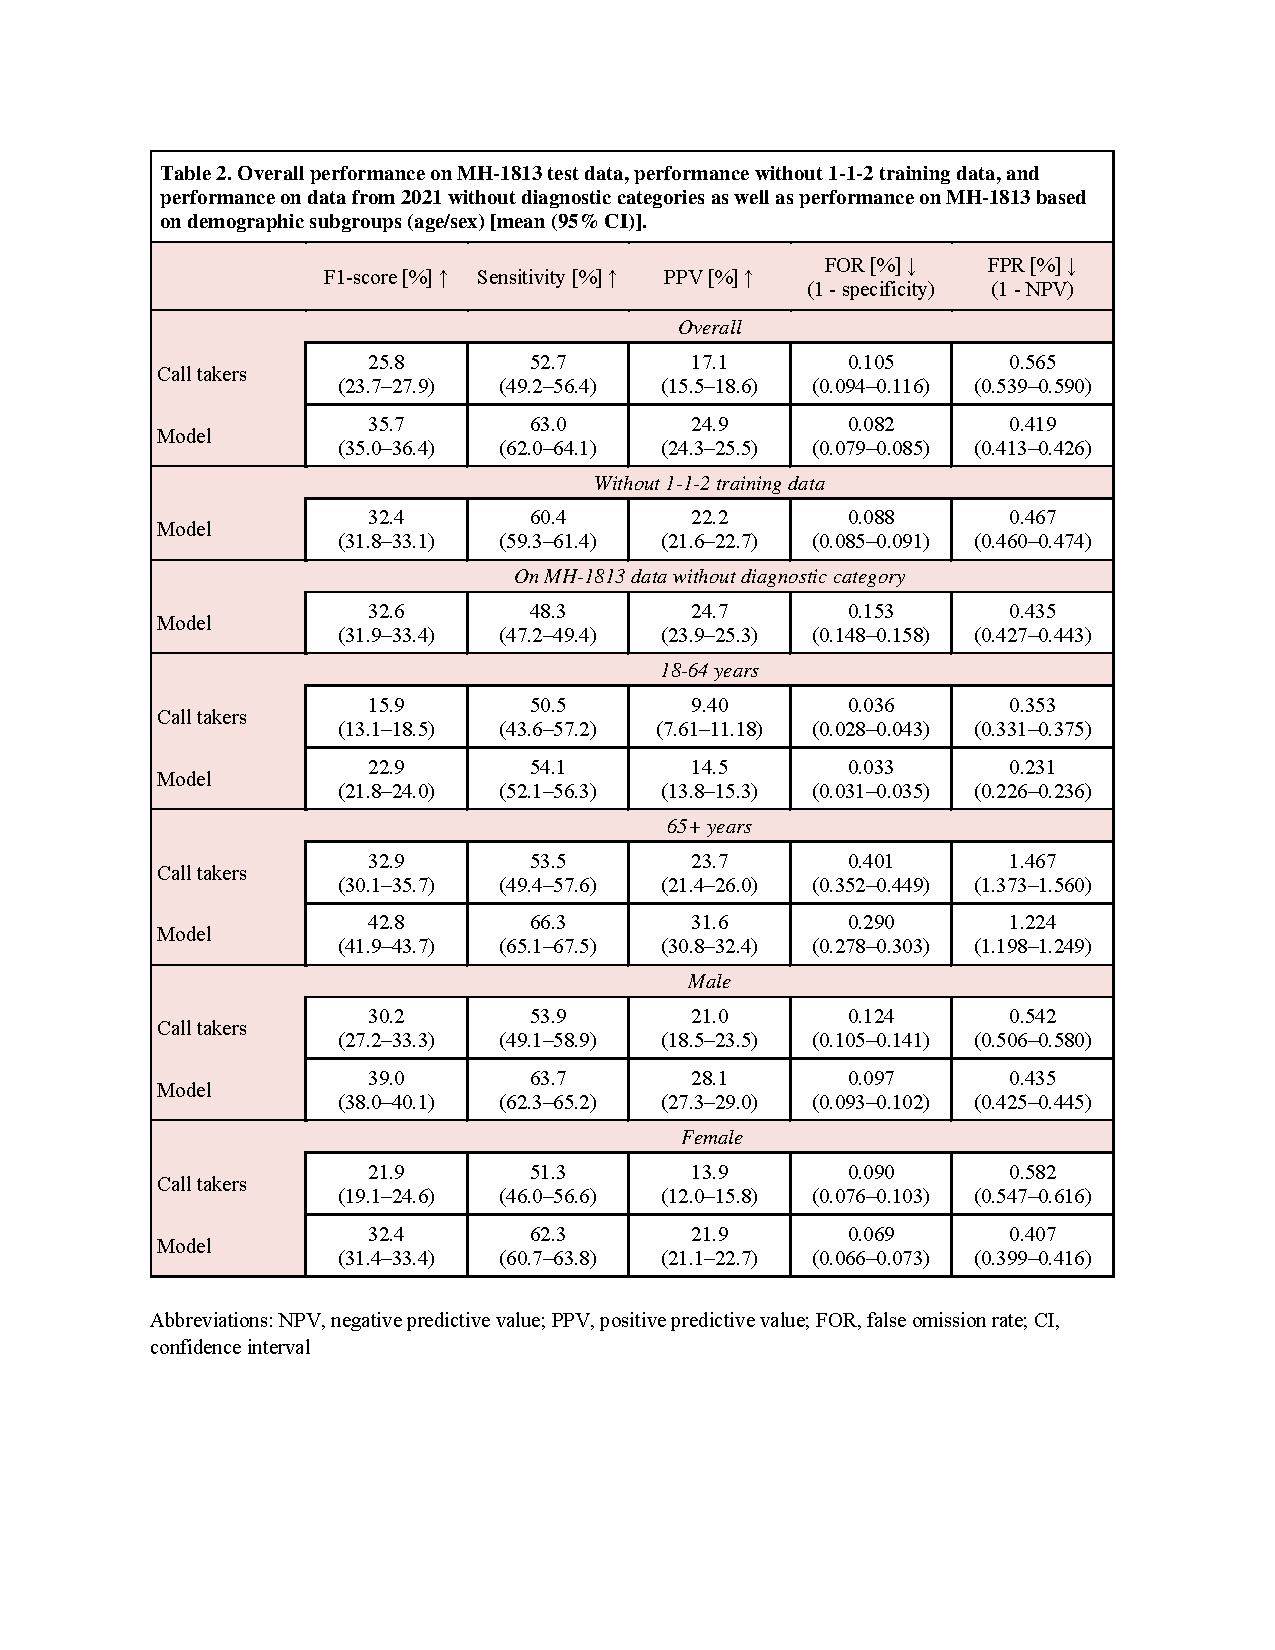
\includegraphics[width=0.3\paperwidth]{../graphics/paper_retrospective/table2.pdf}
    % \end{figure}
\end{frame}


\begin{frame}
    \frametitle{Model performance}
    \begin{figure}
        \centering
        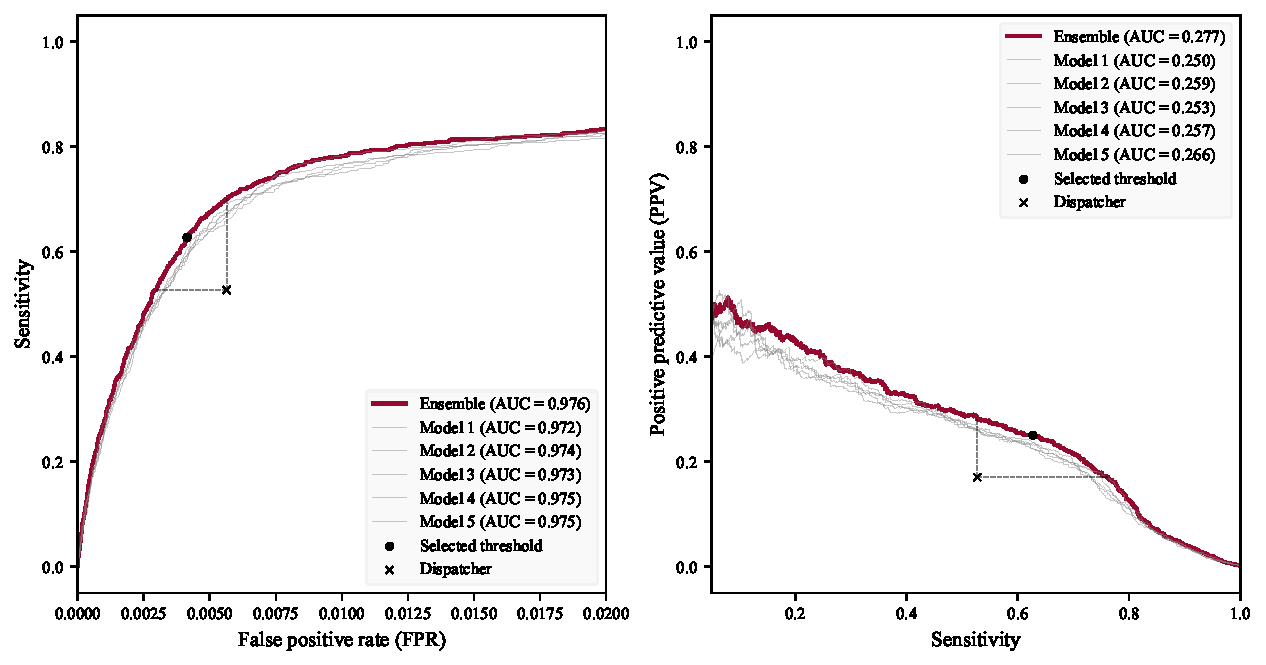
\includegraphics[width=0.65\paperwidth]{../graphics/paper_retrospective/figure1.pdf}
        \caption{Left, the ROC curve and, right, PPV-sensitivity curve (precision-recall curve). Models 1-5 are the individual models that make up the ensemble model.}
    \end{figure}
\end{frame}


\begin{frame}
    \frametitle{Model performance}
    \begin{figure}
        \centering
        \caption{Confusion matrices of predictions for call takers and the model on the test set. Numbers for the model are given as the rounded mean over eleven runs.}
        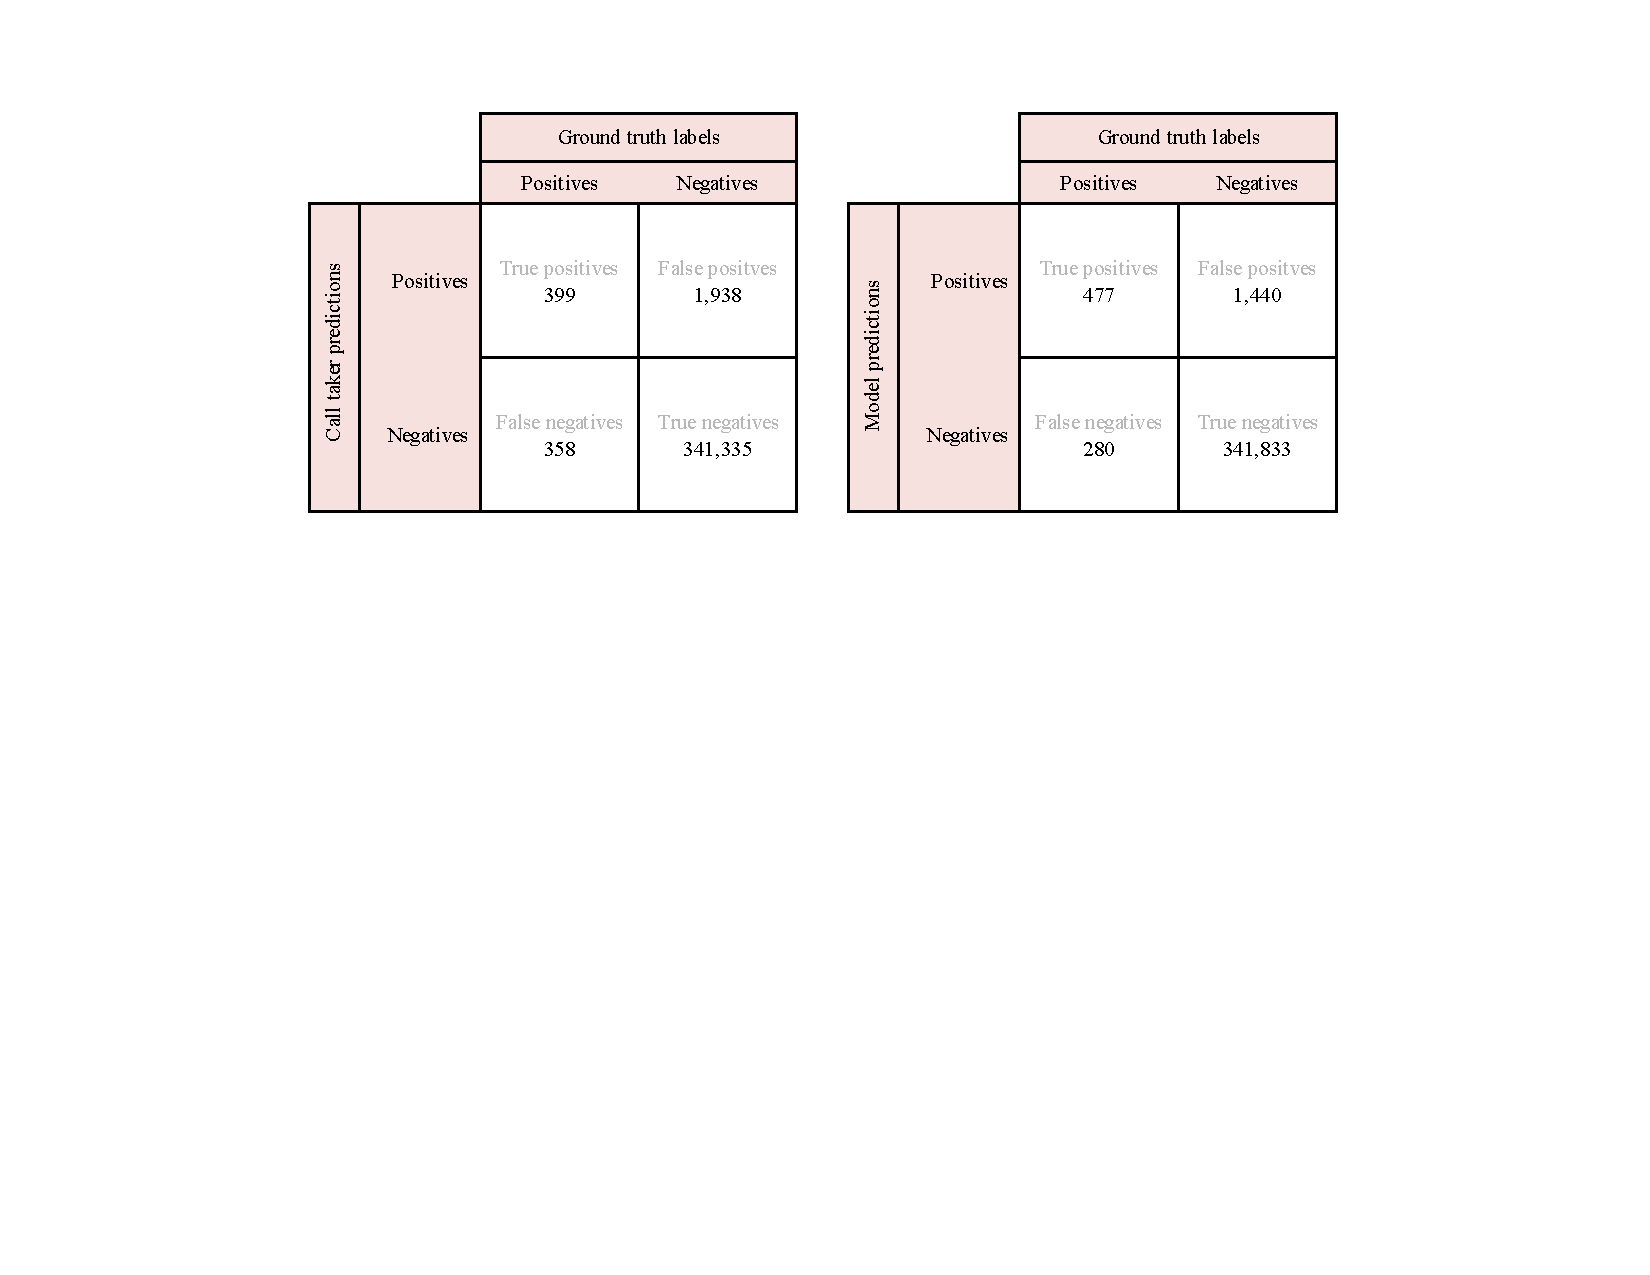
\includegraphics[width=0.85\paperwidth]{../graphics/paper_retrospective/figure2.pdf}
    \end{figure}
\end{frame}


\begin{frame}
    \frametitle{Which features are important?}
    Let $z^{(n, d, w)}$ be the logit output of model $n$ in the ensemble for transcript $d$ when the word $w$ is occluded. For transcript $d$, we computed the word impact score $i^{(d, w)}$ as the mean difference between the logit before and after occlusion.
    %
    \begin{equation}
        i^{(d,w)} = \frac{1}{N_d} \sum_{n=1}^{N_d} \left( z^{(n, d)} - z^{(n, d, w)} \right) \enspace .
    \end{equation}
    %
    To select words for inspection, we computed a word-rank score, $r^{(w)}$, as the sum of the signed squares of the impact:
    %
    \begin{equation}
        r^{(w)} = \sum_{d=1}^{N} \text{sign}\left( i^{(d, w)} \right) \left( i^{(d,w)}\right) ^2 \enspace .
    \end{equation}
    %
    Squaring $i^{(d,w)}$ favors rare features with a high impact over common features with a low impact.
\end{frame}


\begin{frame}
    \frametitle{Which features are important?}
    \begin{table}[t]
        \centering
        % \caption[Words with the largest positive and negative ranking score in calls predicted as stroke and non-stroke, respectively.]{English translation of words with the largest positive and negative ranking score in calls predicted as stroke and non-stroke, respectively. For this analysis, we used the model with the median F1-score out of 11 randomly seeded runs.}
        % \label{tab_retrospective:table3-occlusion-analysis}
        \resizebox*{0.98\textwidth}{!}{%
        \begin{tabular}{l|lr|lr}
            \toprule
                        & \multicolumn{2}{c|}{Positive ranking score, $r^{(w)}$} & \multicolumn{2}{c}{Negative ranking score, $r^{(w)}$} \\
            \midrule
                        & \multicolumn{2}{c|}{Stroke predictions, $D=1,897$} & \multicolumn{2}{c}{Non-stroke predictions, $D=342,133$} \\
            \midrule
                        & Word, $w$ \textit{(translated)} & Occurrences, $D^{(w)}$ & Word, $w$ \textit{(translated)} & Occurrences, $D^{(w)}$ \\
            \midrule
            1.  & Ambulance & 1,680 & Tetanus & 4,378 \\        
            2.  & Blood clot & 895 & Pregnant & 8,749 \\        
            3.  & Left & 1,108 & Cut & 7,592 \\        
            4.  & Right & 1,050 & Bandage & 4,561 \\        
            5.  & Double vision & 84 & Amager (a location) & 23,776 \\        
            6.  & The words & 344 & O'clock & 94,436 \\        
            7.  & Suddenly & 783 & The emergency room & 42,809 \\        
            8.  & Arm & 709 & The police & 2,903 \\        
            9.  & Side & 1,139 & Swollen & 60,559 \\        
            10. & Stroke & 117 & Over the counter (OTC) & 4,641 \\        
            11. & Double & 113 & The neck & 30,151 \\        
            12. & Control & 134 & Fever & 112,586 \\        
            13. & Call & 39 & Prescription & 5,450 \\        
            14. & Numb & 94 & Centimeter & 12,026 \\        
            15. & Minutes & 763 & The knee & 8,875 \\        
            16. & Difficulties speaking & 44 & The pharmacy & 10,085 \\        
            17. & Hemorrhagic stroke & 133 & The stomach & 42,105 \\        
            18. & Hand & 297 & Psychiatric & 3,688 \\        
            19. & The ambulance & 521 & Pneumonia & 7,597 \\        
            20. & Slurred speech & 58 & Stomach pain & 10,551 \\        
            21. & Blood clots & 224 & Stool & 19,155 \\        
            22. & Fast & 663 & The ribs & 3,928 \\        
            23. & Express & 44 & Bleed & 10,501 \\        
            24. & Blood thinner & 259 & Bleeding & 24,313 \\        
            25. & Incoherent & 15 & Ribs & 2,941 \\        
            26. & Lopsided & 211 & Broken & 19,415 \\        
            27. & Reduced & 528 & Inflammation & 10,050 \\        
            28. & Hangs & 628 & Common cold & 8,127 \\        
            29. & Transient & 48 & Morning or morrow & 78,558 \\        
            30. & Not making sense & 14 & Swelling & 17,762 \\        
            \bottomrule
        \end{tabular}%
        }
    \end{table}
    % \begin{figure}
    %     \centering
    %     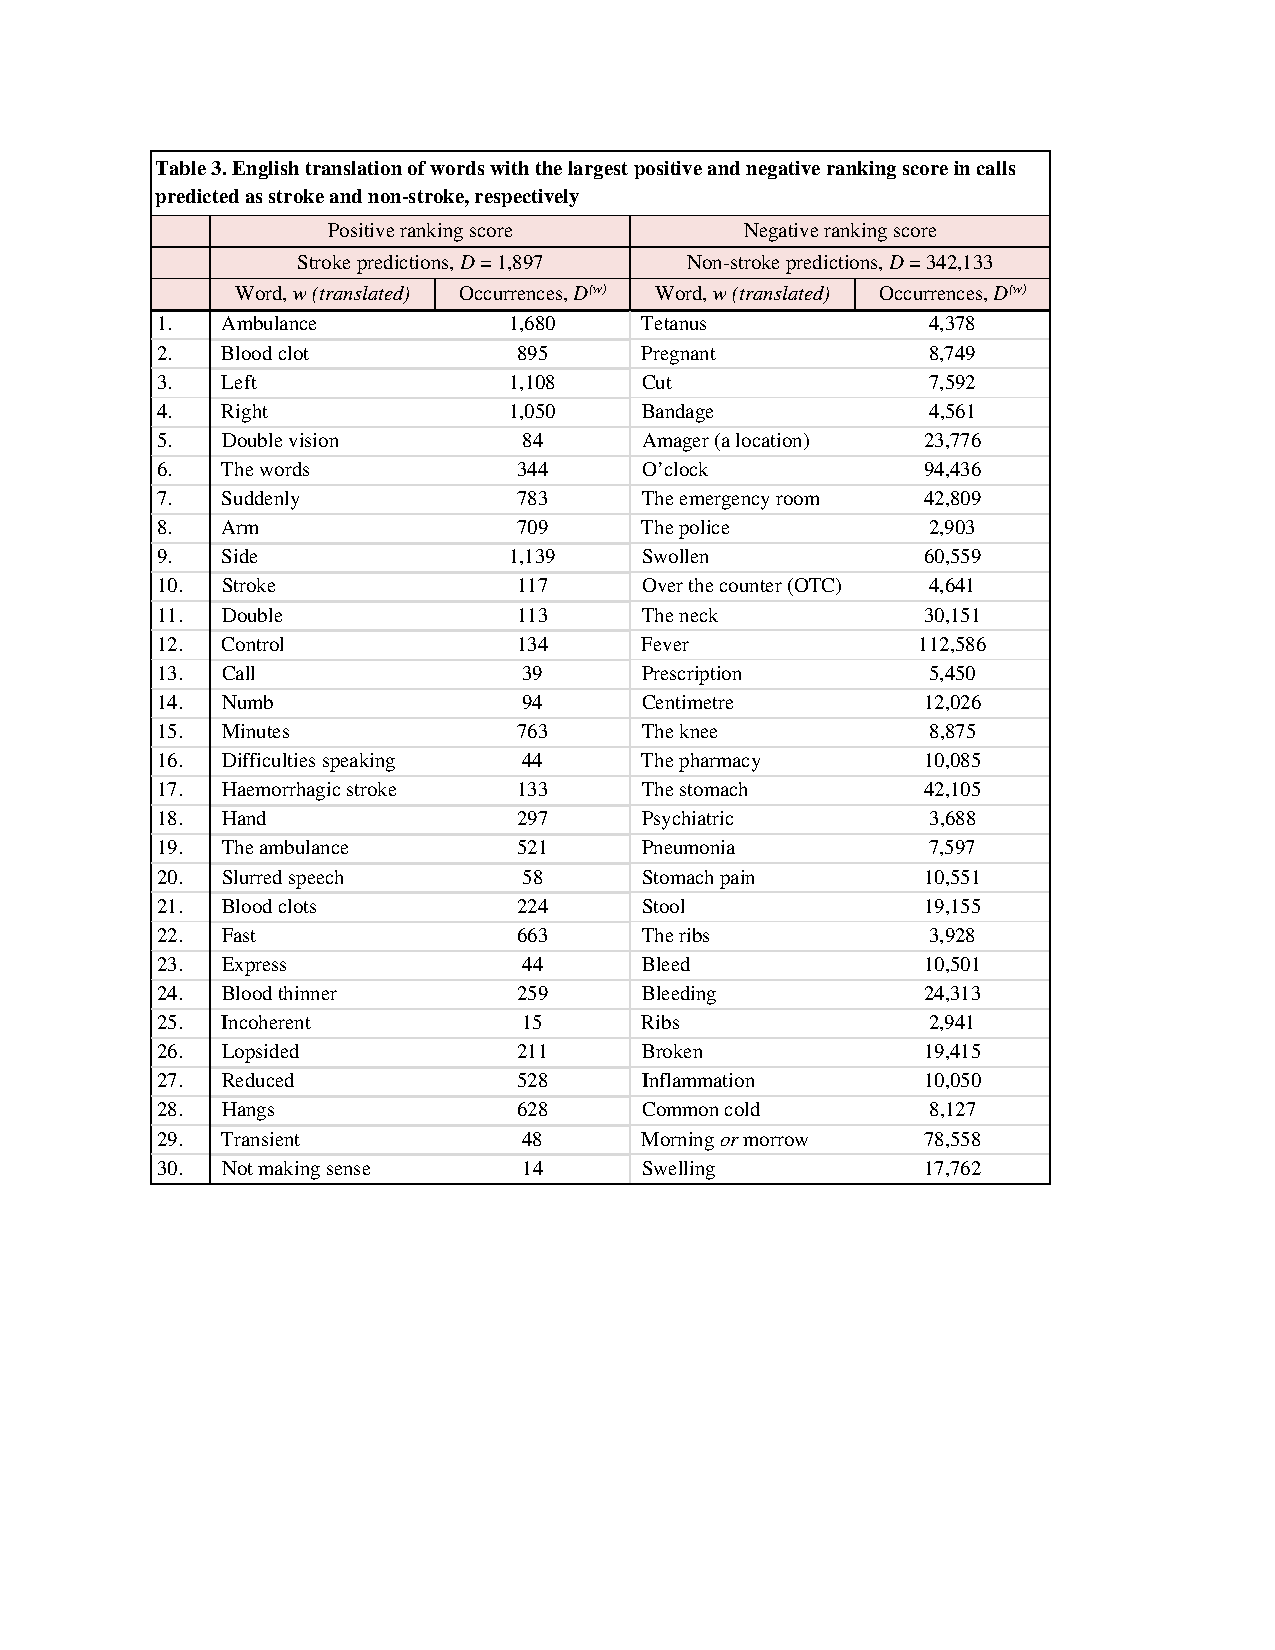
\includegraphics[width=0.4\paperwidth]{../graphics/paper_retrospective/table3.pdf}
    % \end{figure}
\end{frame}


\begin{frame}
    \frametitle{Simulated prospective study}
    \begin{enumerate}
        \item[I.] {\color{dtured}When} is the model prediction presented to the call-taker?
        \begin{enumerate}
            \item[1.] Notify the call-taker {\color{dtured}after the call ends}.
            \item[2.] Notify the call-taker {\color{dtured}during the call}.
        \end{enumerate}
        \item[II.] {\color{dtured}How} does prediction influence the diagnostic code the call-taker assigns to the call?
        \begin{enumerate}[label=\Alph*.]
            \item[A.] Call-takers mirror model positives.
            \item[B.] Call-takers mirror model negatives.
            \item[C.] Call-takers mirror model predictions (corresponds to main results of the model itself).
        \end{enumerate}
    \end{enumerate}
    \vspace{1em}
    To simulate the online scenario (2.), we stream the transcript to the model and make predictions every 50 words. 
    A stroke positive is triggered only when three consecutive positive predictions are made. 
    This is similar to the strategy implemented for a previous RCT on cardiac arrest \cite{cite15}.

        % %
        % Option 1 is identical to the method used in the main study. In option 2, predictions are made during the call based only on partial transcriptions. We implemented option 2 in such a manner that the model predicted every time 50 new words were transcribed and added to the transcript. A stroke positive was triggered only when three consecutive positive predictions were made (i.e., without intermediate negative stroke predictions). In other words, the sigmoid activation of the model had to remain above 0.5 for three consecutive predictions, for example, after 150, 200, and 250 words were transcribed.
        
        % As we can only assume how call takers are influenced by model predictions (II), precisely evaluating the hypothetical performance of call takers when supported by a machine learning framework is impossible. Furthermore, option 2 may influence the conversation, further complicating matters. Therefore, we report the results combining the call taker and the model under the following two assumptions:
        % %
\end{frame}


\begin{frame}
    \frametitle{Simulated prospective study}

    \begin{table}
        \centering
        % \caption{Overall performance of model, call-takers and simulated combinations of model and call-takers on MH-1813 test data.}
        % \label{tab_retrospective:tableA9}
        \resizebox*{0.98\textwidth}{!}{%
        \begin{tabular}{c|c|cc|cc|cc}
            \toprule
    
            \textbf{Predictor} & \textbf{Call-taker} & \multicolumn{2}{c|}{\textbf{Model}} & \multicolumn{4}{c}{\textbf{Call-taker supported by the model (simulated)}} \\
            \midrule
            \textbf{When} & \textbf{During call} & \textbf{After call} & \textbf{During call} & \textbf{After call} & \textbf{During call} & \textbf{After call} & \textbf{During call} \\
            \midrule
            \textbf{Method} & - & - & - & \textbf{neg $\rightarrow$ pos} & \textbf{neg $\rightarrow$ pos} & \textbf{pos $\rightarrow$ neg} & \textbf{pos $\rightarrow$ neg} \\
            \midrule
    
            \makecell[l]{\textbf{F1-score} [\%] $\uparrow$}                   & \makecell[c]{25.8 \\ (23.7-27.9)} & \makecell[c]{35.7 \\ (35.0-36.4)} & \makecell[c]{33.1 \\ (32.4-33.7)} & \makecell[c]{28.9 \\ (28.3-29.5)} & \makecell[c]{27.6 \\ (27.0-28.1)}  & \makecell[c]{33.3 \\ (32.5-34.1)}& \makecell[c]{32.7 \\ (31.8-33.5)} \\
            \midrule
            \makecell[l]{\textbf{Sensitivity} [\%] $\uparrow$}                & \makecell[c]{52.7 \\ (49.2-56.4)} & \makecell[c]{63.0 \\ (62.0-64.1)} & \makecell[c]{58.7 \\ (57.7-59.8)} & \makecell[c]{72.4 \\ (71.5-73.3)} & \makecell[c]{72.3 \\ (71.4-73.3)} & \makecell[c]{43.4 \\ (42.3-44.5)} & \makecell[c]{39.1 \\ (38.1-40.1)} \\
            \midrule
            \makecell[l]{\textbf{PPV} [\%] $\uparrow$}                        & \makecell[c]{17.1 \\ (15.5-18.6)} & \makecell[c]{24.9 \\ (24.3-25.5)} & \makecell[c]{23.0 \\ (22.5-23.6)} & \makecell[c]{18.0 \\ (17.6-18.4)} & \makecell[c]{17.0 \\ (16.7-17.4)} & \makecell[c]{27.0 \\ (26.3-27.8)} & \makecell[c]{28.1 \\ (27.3-28.9)} \\
            \midrule
            \makecell[l]{\textbf{FOR} [\%] $\downarrow$ \\ (1 - NPV)}         & \makecell[c]{0.105 \\ (0.094-0.116)} & \makecell[c]{0.082 \\ (0.079-0.085)} & \makecell[c]{0.091 \\ (0.088-0.094)} & \makecell[c]{0.061 \\ (0.059-0.064)} & \makecell[c]{0.061 \\ (0.059-0.064)} & \makecell[c]{0.125 \\ (0.121-0.129)} & \makecell[c]{0.134 \\ (0.131-0.138)} \\
            \midrule
            \makecell[l]{\textbf{FPR} [\%] $\downarrow$ \\ (1 - specificity)} & \makecell[c]{0.565 \\ (0.539-0.590)} & \makecell[c]{0.419 \\ (0.413-0.426)} & \makecell[c]{0.432 \\ (0.426-0.439)} & \makecell[c]{0.726 \\ (0.717-0.735)} & \makecell[c]{0.776 \\ (0.767-0.786)} & \makecell[c]{0.258 \\ (0.253-0.263)} & \makecell[c]{0.221 \\ (0.216-0.226)} \\
    
            \bottomrule
        \end{tabular}%
        }
    \end{table}

\end{frame}


\begin{frame}
    \frametitle{Fine-tuning a large language model}
    \begin{table}
        \centering
        % \caption[Overall performance on MH-1813 test data for a fine"=tuned BERT model.]{Overall performance on MH-1813 test data for the fine-tuned BERT model described in the revised discussion of the paper. Includes performance of the call-takers and the multi-layer perceptron (MLP) from the main manuscript for ease of comparison [mean (95\% CI)]. NPV: negative predictive value, PPV: positive predictive value, FOR: false omission rate, CI: confidence interval.}
        % \label{tab_retrospective:tableA8}
        \resizebox*{0.98\textwidth}{!}{%
        \begin{tabular}{l|ccccc}
            \toprule
            & F1-score [\%] $\uparrow$ & Sensitivity [\%] $\uparrow$ & PPV [\%] $\uparrow$ & \makecell[c]{FOR [\%] $\downarrow$ \\ (1 - NPV)} & \makecell[c]{FPR [\%] $\downarrow$ \\ (1 - specificity)} \\
            \midrule
            & \multicolumn{5}{c}{\textit{Overall}} \\
            \midrule
            
            Call-takers                             & \makecell[c]{25.8 \\ (23.7-27.9)} & \makecell[c]{52.7 \\ (49.2-56.4)} & \makecell[c]{17.1 \\ (15.5-18.6)} & \makecell[c]{0.105 \\ (0.094-0.116)} & \makecell[c]{0.565 \\ (0.539-0.590)} \\
            \midrule
            \makecell[l]{MLP}                       & \makecell[c]{35.7 \\ (35.0-36.4)} & \makecell[c]{63.0 \\ (62.0-64.1)} & \makecell[c]{24.9 \\ (24.3-25.5)} & \makecell[c]{0.082 \\ (0.079-0.085)} & \makecell[c]{0.419 \\ (0.413-0.426)} \\
            \midrule
            \makecell[l]{BERT \\ (fine"=tuned)}      & \makecell[c]{33.8 \\ (31.5-36.2)} & \makecell[c]{57.5 \\ (53.9-60.9)} & \makecell[c]{23.9 \\ (21.9-25.9)} & \makecell[c]{0.094 \\ (0.084-0.104)} & \makecell[c]{0.403 \\ (0.381-0.424)} \\
     
            \bottomrule
        \end{tabular}%
        }
    \end{table}
\end{frame}


\begin{frame}
    \frametitle{Future work}
    \begin{itemize}
        \item Self-supervised learning directly from audio data.
        \item Investigate learning to defer to predict methods \cite{verma_calibrated_2022}.
    \end{itemize}
\end{frame}


% End slide
\frame{\centering\Huge Thank you for your attention}

% Bibliography slide
\begin{frame}[allowframebreaks]{Bibliography}\printbibliography\end{frame}

% !TEX root = ../presentation.tex
% !BIB program = biber
% !TEX program = xelatex

\section[short]{hierarchical vaes know what they don't know}

\begin{frame}
    \frametitle{Results on diverse datasets}
    \begin{columns}
        \begin{column}{0.45\textwidth}
            \hfill
            \begin{table}[t]
                \centering
                \resizebox{0.9\textwidth}{!}{%
                \begin{tabular}{llrrr}
                    \toprule
                    OOD dataset & Metric & AUROC$\uparrow$ & AUPRC$\uparrow$ & FPR80$\downarrow$ \\
                    \midrule
                    \multicolumn{5}{c}{\textbf{Trained on CIFAR10}} \\
                    \midrule
                    SVHN          &  $LLR^{>2}$  &  0.811  &  0.837  &  0.394  \\
                    CIFAR10       &  $LLR^{>1}$  &  0.469  &  0.479  &  0.835  \\
                    \midrule
                    \multicolumn{5}{c}{\textbf{Trained on SVHN}} \\
                    \midrule
                    CIFAR10            &  $LLR^{>1}$       &  $0.939$  &  $0.950$  &  $0.052$  \\
                    SVHN               &  $LLR^{>1}$       &  $0.489$  &  $0.484$  &  $0.799$  \\
                    \bottomrule
                \end{tabular}
                }
            \end{table}
            \hfill
        \end{column}
        \begin{column}{0.55\textwidth}
            \hfill
            \begin{table}[t]
                \centering
                \resizebox{0.9\textwidth}{!}{%
                \begin{tabular}{llrrr}
                    \toprule
                    OOD dataset & Metric & AUROC$\uparrow$ & AUPRC$\uparrow$ & FPR80$\downarrow$ \\
                    \midrule
                    \multicolumn{5}{c}{\textbf{Trained on FashionMNIST}} \\
                    \midrule
                    MNIST                    & $LLR^{>1}$             &  0.986  &  0.987  &  0.011 \\
                    notMNIST                 &  $LLR^{>1}$            &  0.998  &  0.998  &  0.000 \\
                    KMNIST                   &  $LLR^{>1}$            &  0.974  &  0.977  &  0.017 \\
                    Omniglot28x28            &  $LLR^{>2}$            &  1.000  &  1.000  &  0.000 \\
                    Omniglot28x28Inverted    &  $LLR^{>1}$            &  0.954  &  0.954  &  0.050 \\
                    SmallNORB28x28           &  $LLR^{>2}$            &  0.999  &  0.999  &  0.002 \\
                    SmallNORB28x28Inverted   &  $LLR^{>2}$            &  0.941  &  0.946  &  0.069 \\
    {\color{black!60}FashionMNIST}             &  $LLR^{>1}$            &  0.488  &  0.496  &  0.811 \\
                    \midrule
                    \multicolumn{5}{c}{\textbf{Trained on MNIST}} \\
                    \midrule
                    FashionMNIST                   &  $LLR^{>1}$  &  $0.999$  &  $0.999$  &  $0.000$ \\
                    notMNIST                       &  $LLR^{>1}$  &  $1.000$  &  $0.999$  &  $0.000$ \\
                    KMNIST                         &  $LLR^{>1}$  &  $0.999$  &  $0.999$  &  $0.000$ \\
                    Omniglot28x28                  &  $LLR^{>1}$  &  $1.000$  &  $1.000$  &  $0.000$ \\
                    Omniglot28x28Inverted          &  $LLR^{>1}$  &  $0.944$  &  $0.953$  &  $0.057$ \\
                    SmallNORB28x28                 &  $LLR^{>1}$  &  $1.000$  &  $1.000$  &  $0.000$ \\
                    SmallNORB28x28Inverted         &  $LLR^{>1}$  &  $0.985$  &  $0.987$  &  $0.000$ \\
    {\color{black!60}MNIST}                          &  $LLR^{>2}$  &  $0.515$  &  $0.507$  &  $0.792$ \\
                    \bottomrule
                \end{tabular}
                }
            \end{table}
            \hfill
        \end{column}
    \end{columns}
\end{frame}

% ======================================================================================================================

\section{a brief overview of unsupervised speech representation learning}

\begin{frame}
    \frametitle{Types of self-supervised speech representation learning methods}
    
    Schematic of self-supervised methods. Each subfigure illustrates the loss computation for a single time-step. The temporal subscript has been left out for simplicity.

    \begin{figure}
        \centering
        \setlength\tabcolsep{1.5pt}
        \resizebox*{\textheight}{!}{%
        \begin{tabular}{>{\centering\arraybackslash} m{4mm}  >{\centering\arraybackslash} m{0.40\textwidth}|>{\centering\arraybackslash} m{0.40\textwidth}}
            & {\small \textsc{predictive}} & {\small \textsc{masking-based}} \\
            \rotatebox{90}{{\small \textsc{reconstruct}}} & 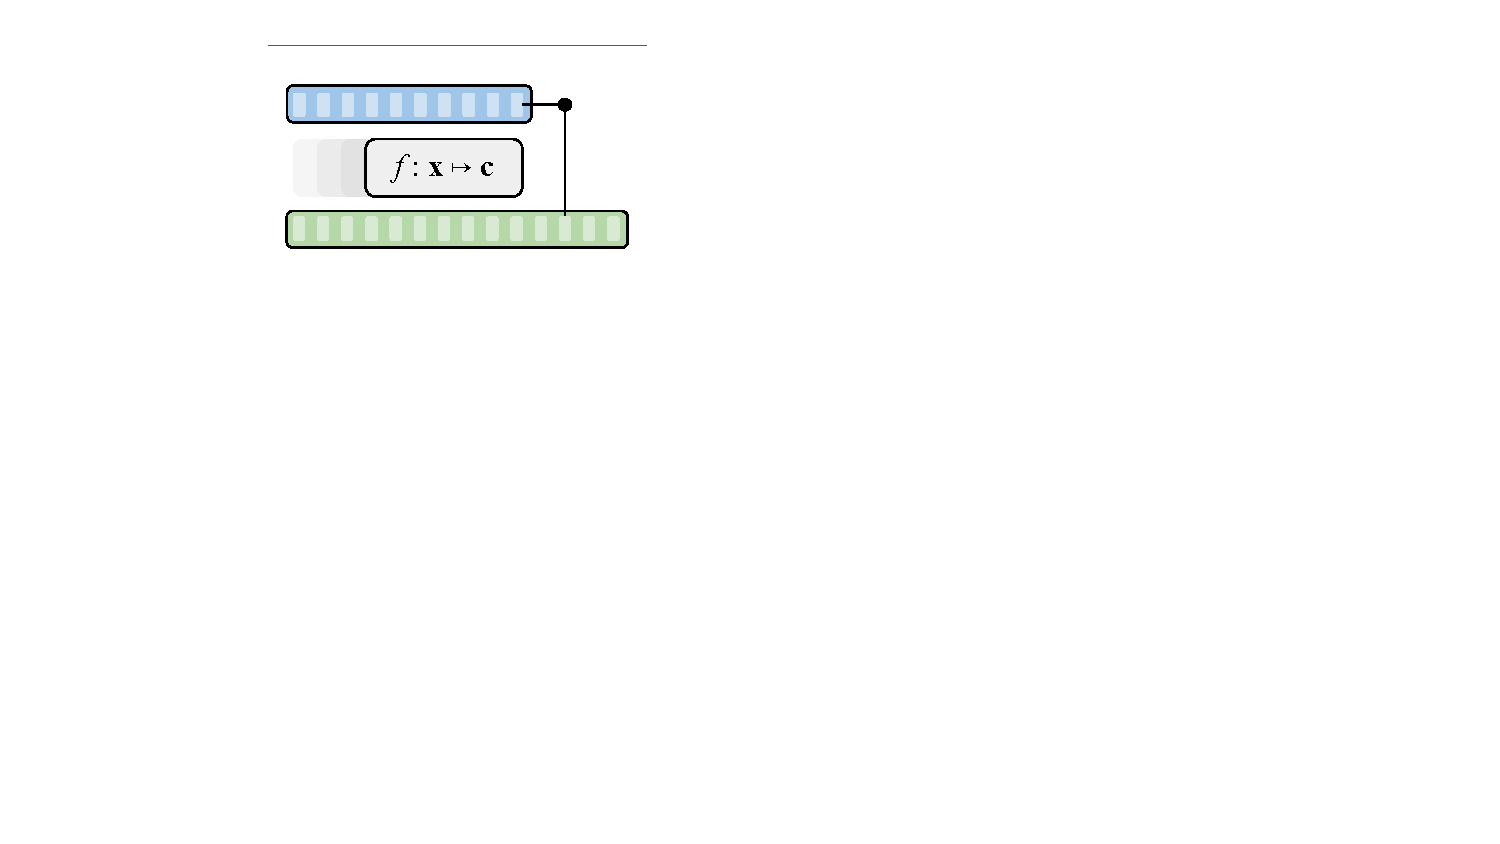
\includegraphics[width=0.40\textwidth]{../graphics/paper_brief/REC_PRD.pdf} & 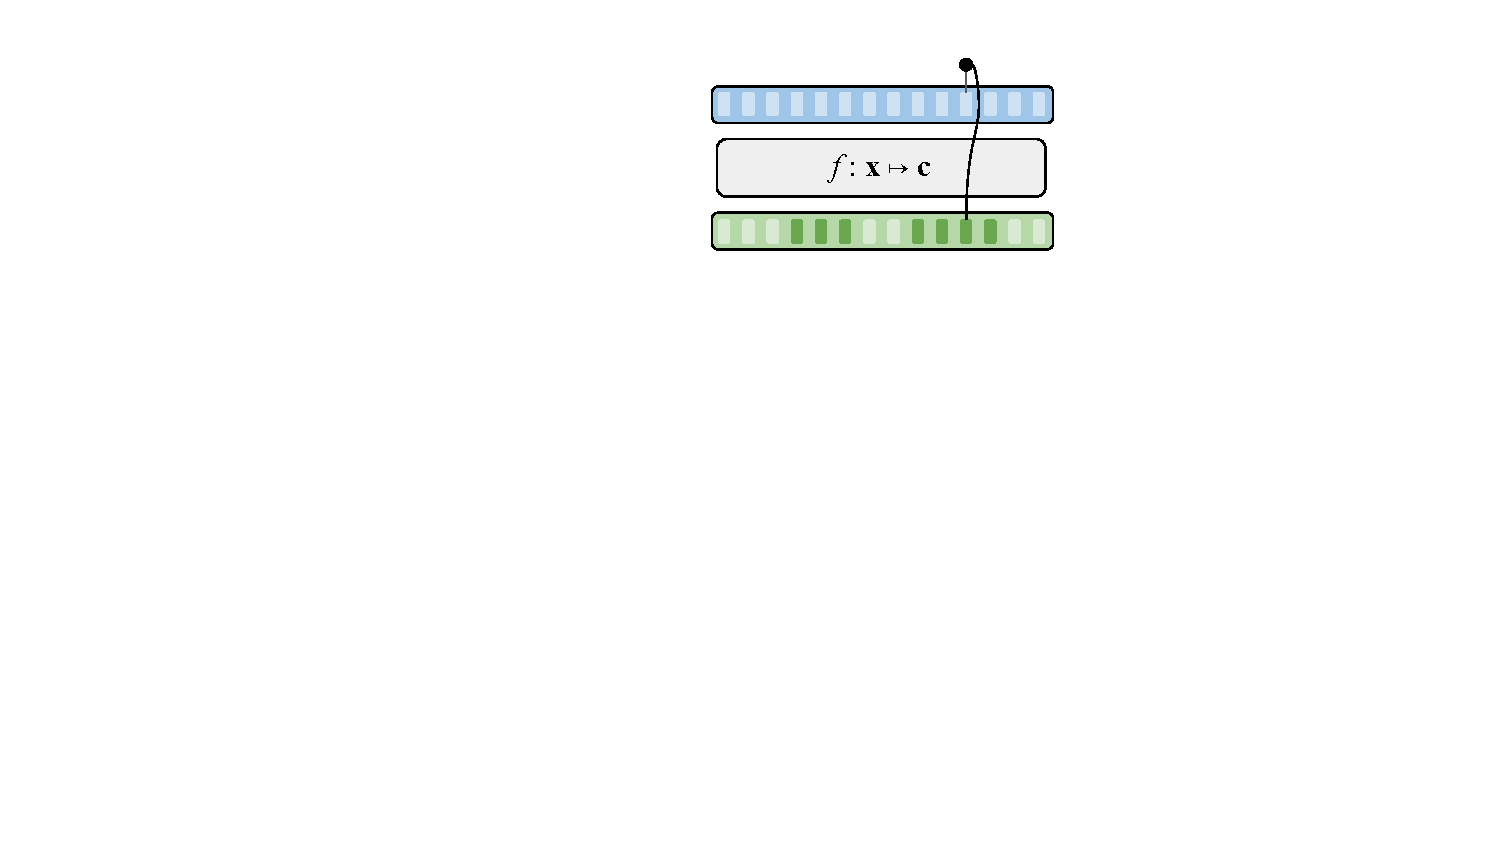
\includegraphics[width=0.40\textwidth]{../graphics/paper_brief/REC_MSK.pdf}  \\
            \midrule
            \rotatebox{90}{{\small \textsc{contrastive}}} & 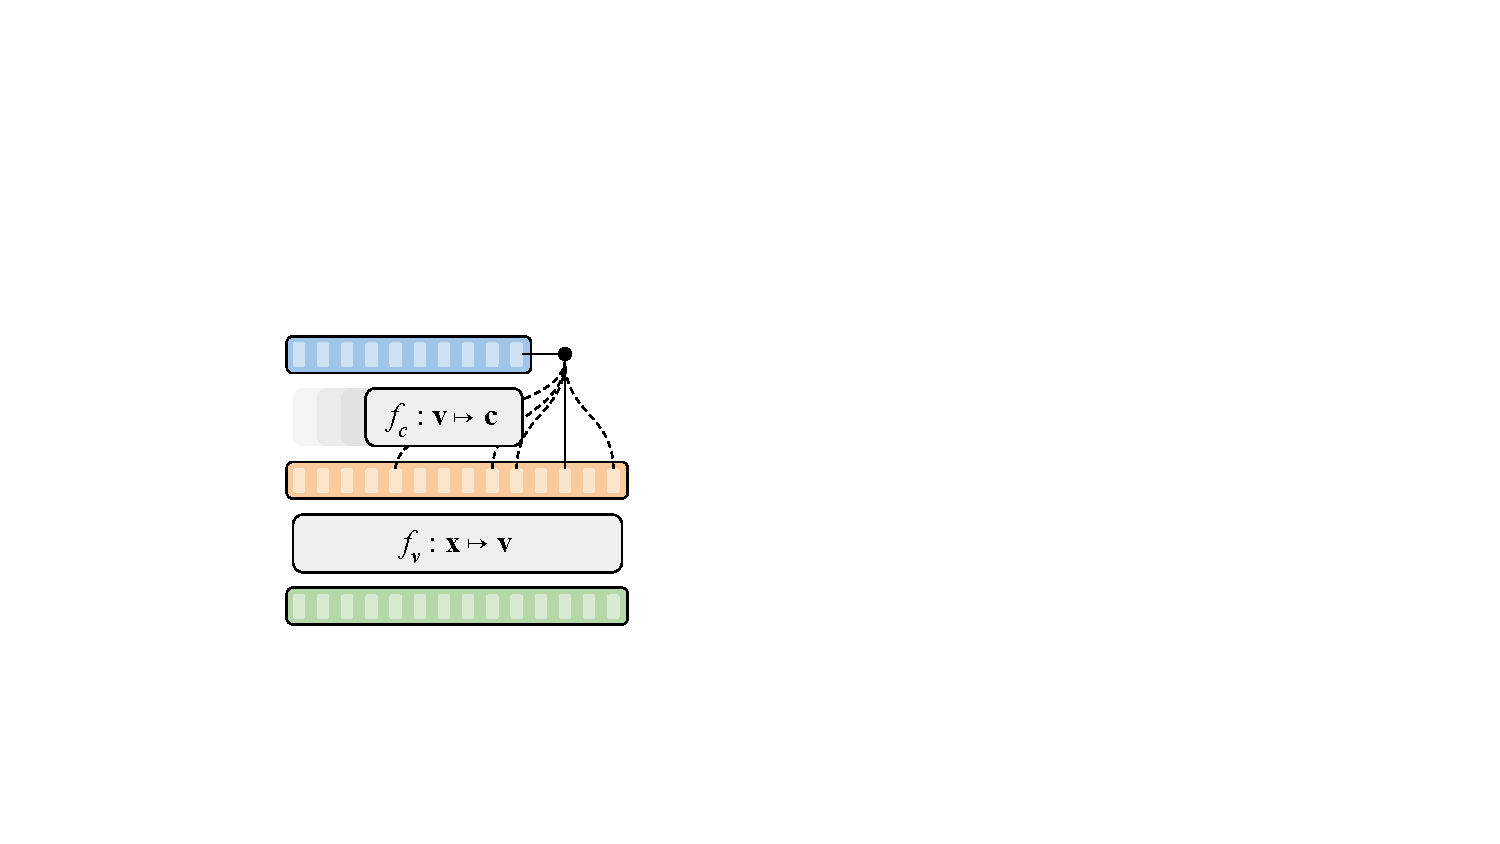
\includegraphics[width=0.40\textwidth]{../graphics/paper_brief/CON_PRD.pdf} & 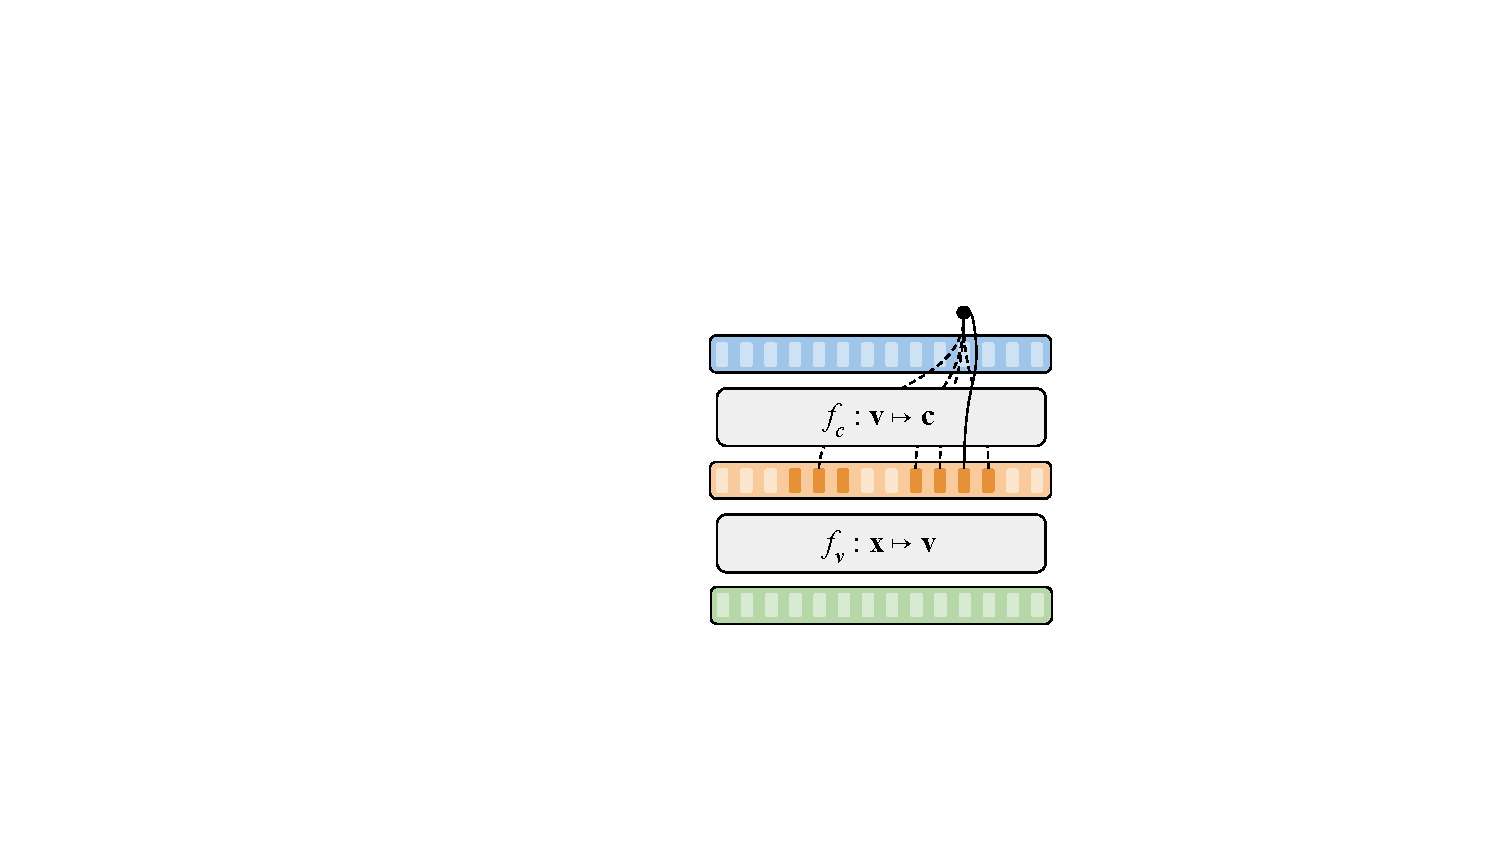
\includegraphics[width=0.40\textwidth]{../graphics/paper_brief/CON_MSK.pdf}
        \end{tabular}
        }
    \end{figure}
\end{frame}


\begin{frame}
    \frametitle{Overview: Representation Learning for Speech}

    \begin{columns}

        \begin{column}{0.4\textwidth}
            \begin{itemize}
                \item We focus on two primary categories:
                \begin{itemize}
                    \item Self-supervised learning (SSL)
                    \item Probabilistic latent variable models (LVMs)
                \end{itemize}
                \item Recent developments have been driven by self-supervised learning.
                \item A model-by-model overview: Focus on speech recognition.
            \end{itemize}
        \end{column}

        \begin{column}{0.6\textwidth}

            \begin{tikzpicture}
                \only<1->{
                    \node[anchor=south west,inner sep=0] (A) at (0,0) {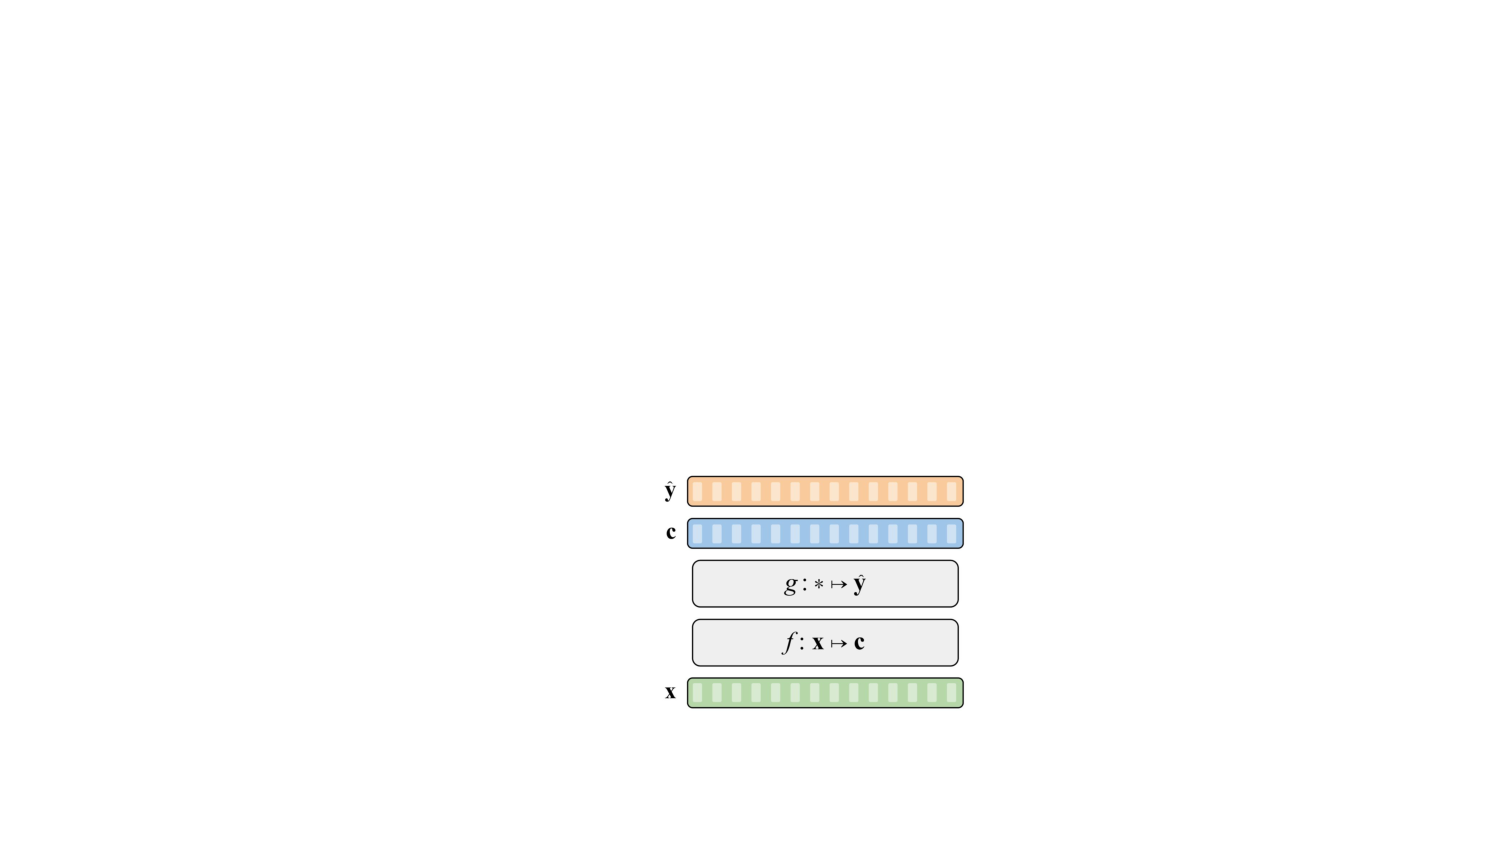
\includegraphics[height=0.4\textheight]{figures/brief-paradigms-ssl.pdf}};
                    \node[anchor=south west,inner sep=0] (B) at (4.2,0) {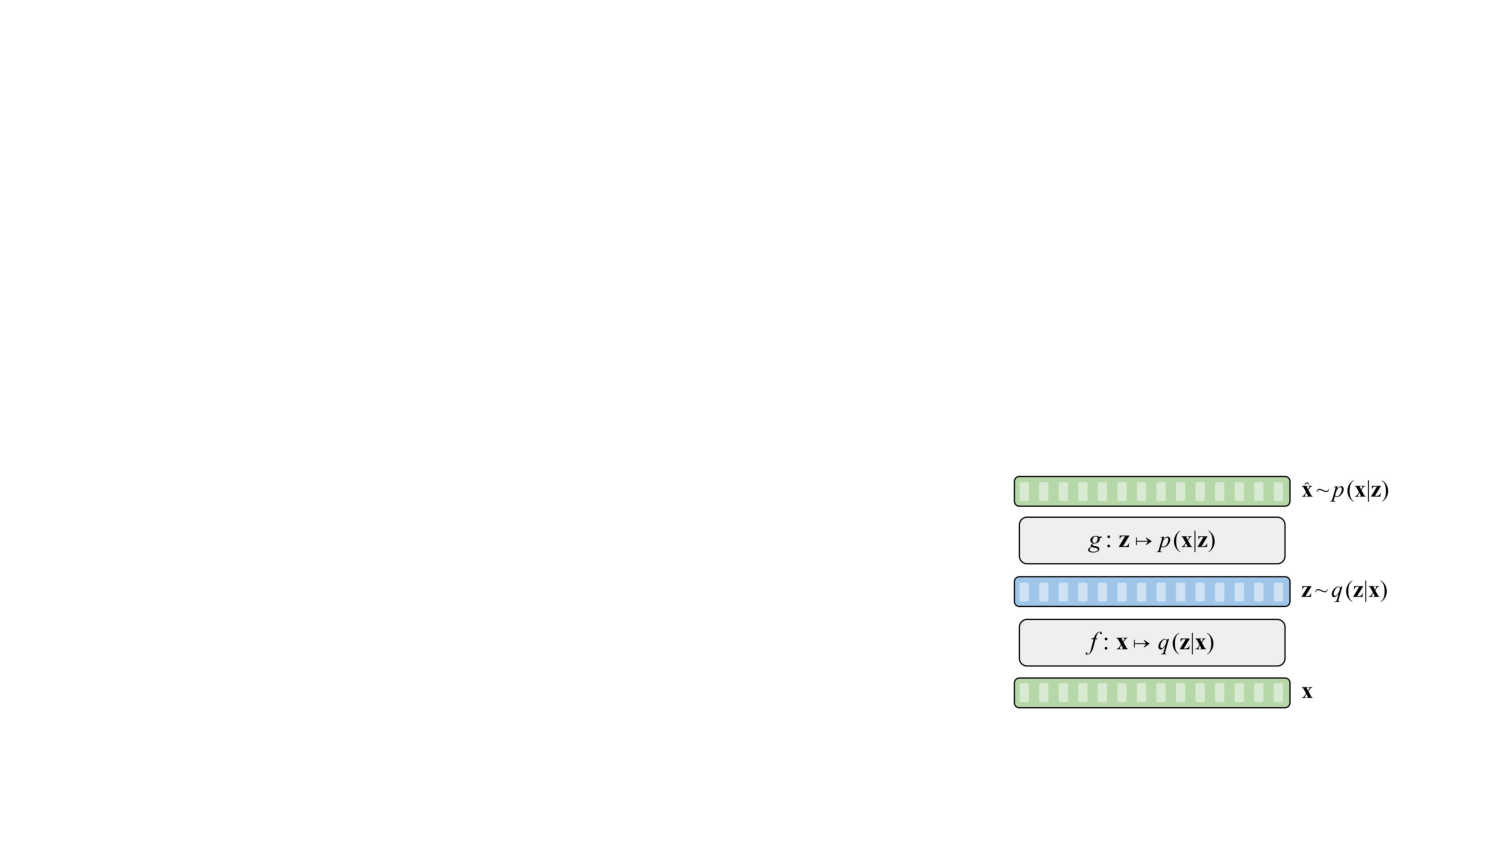
\includegraphics[height=0.4\textheight]{figures/brief-paradigms-lvm-2.pdf}};
                    \fill [draw=none, fill=white, fill opacity=0.7] (B.north west) -- (B.north east) -- (B.south east) -- (B.south west) -- (B.north west) -- cycle;
                }

                \only<2->{
                    \node[anchor=south west,inner sep=0] (A) at (0,0) {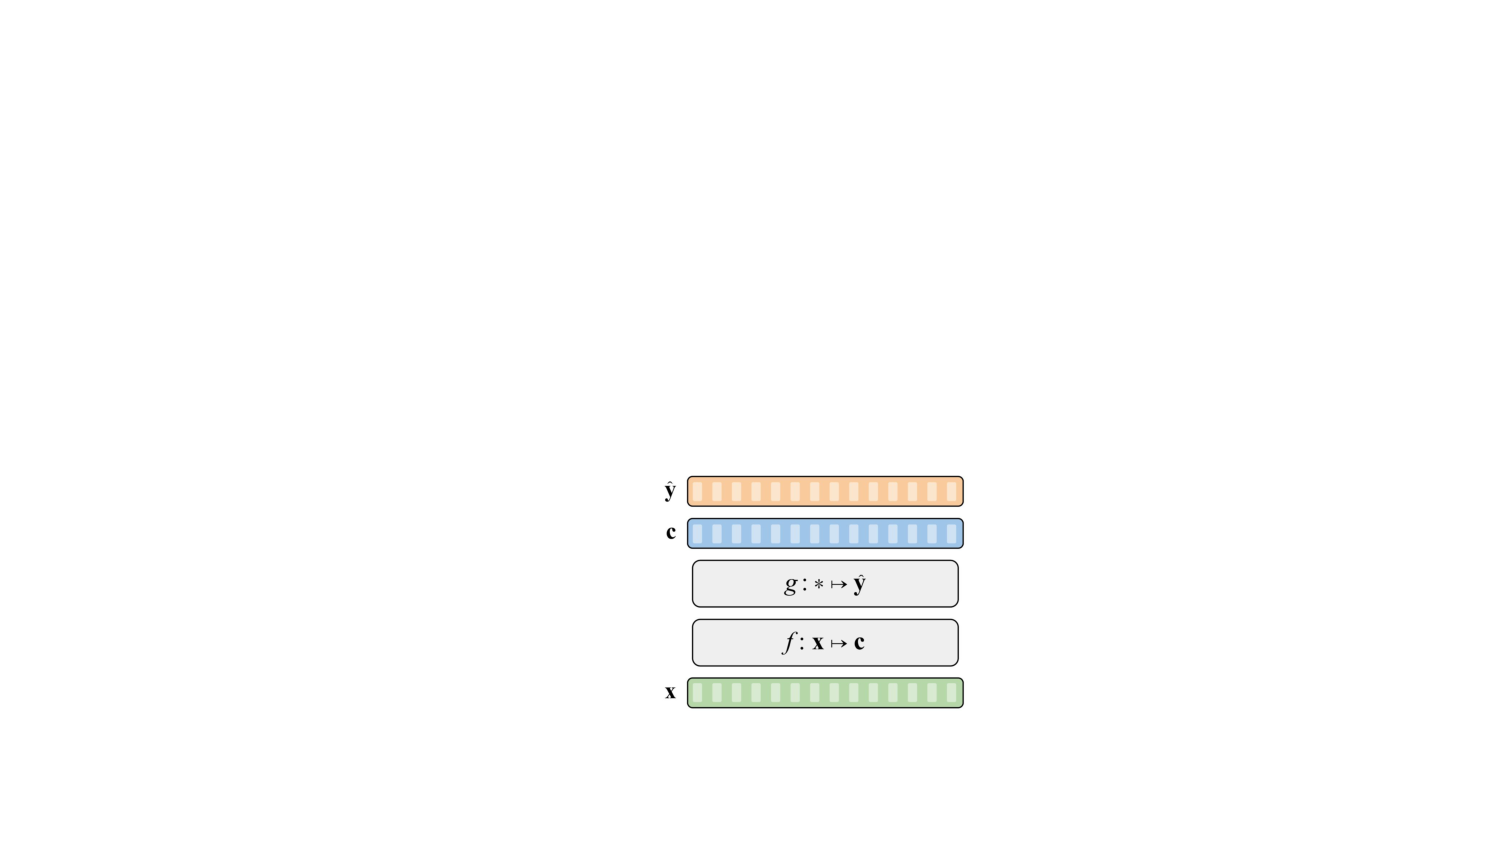
\includegraphics[height=0.4\textheight]{figures/brief-paradigms-ssl.pdf}};
                    \node[anchor=south west,inner sep=0] (B) at (4.2,0) {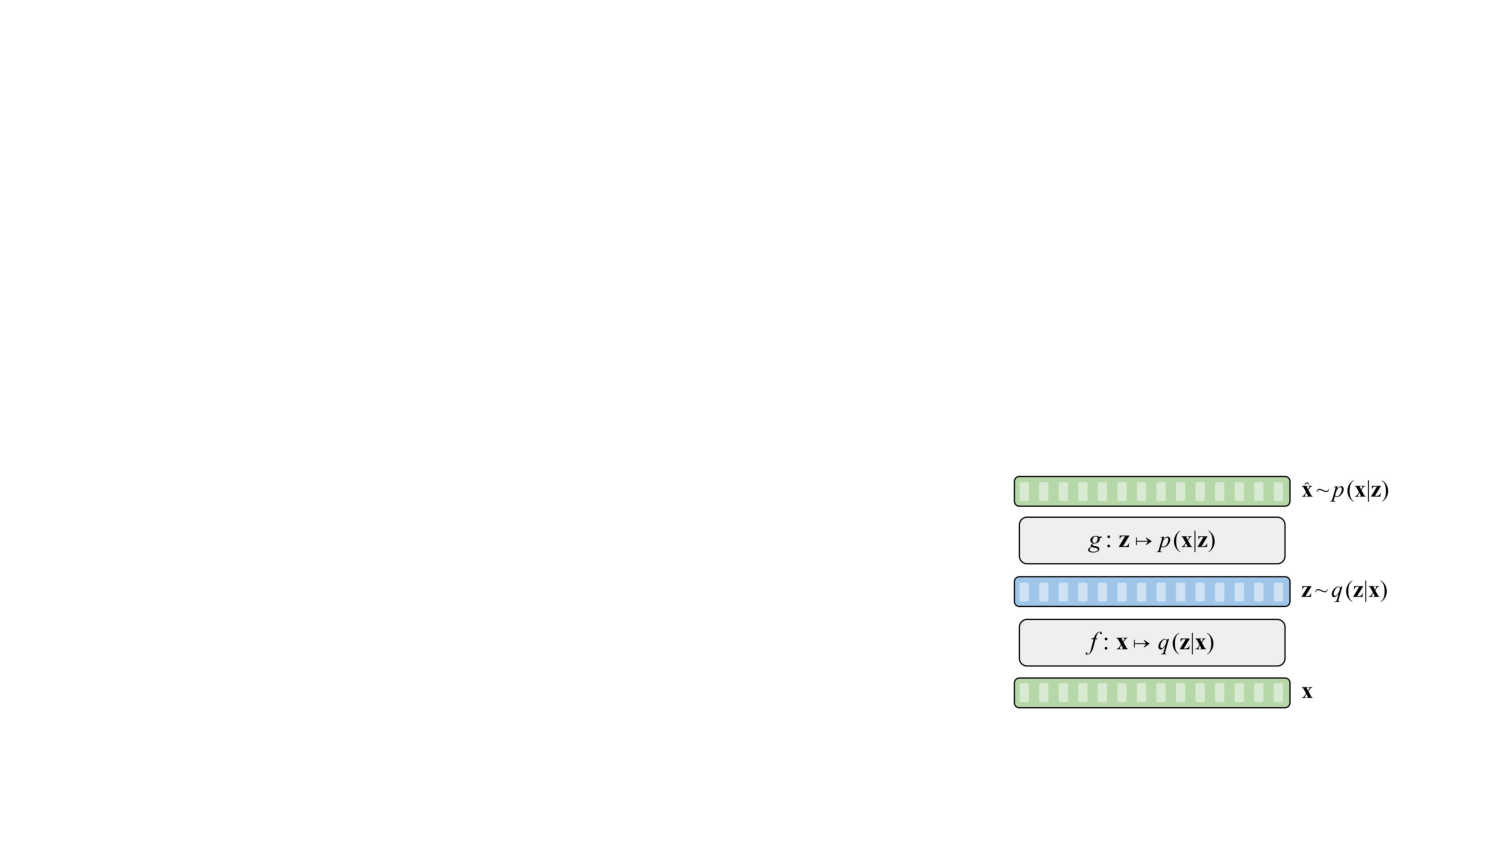
\includegraphics[height=0.4\textheight]{figures/brief-paradigms-lvm-2.pdf}};
                    \fill [draw=none, fill=white, fill opacity=0.7] (A.north west) -- (A.north east) -- (A.south east) -- (A.south west) -- (A.north west) -- cycle;
                }
            \end{tikzpicture}

        \end{column}
        
    \end{columns}
\end{frame}


\begin{frame}
    \frametitle{Graphical models for LVMs}
    % Figure TikZ sources at https://www.overleaf.com/project/61b212df9f315b5aec2b4a33
    \begin{columns}

        \begin{column}{0.5\textwidth}
            \begin{figure}
                \centering
                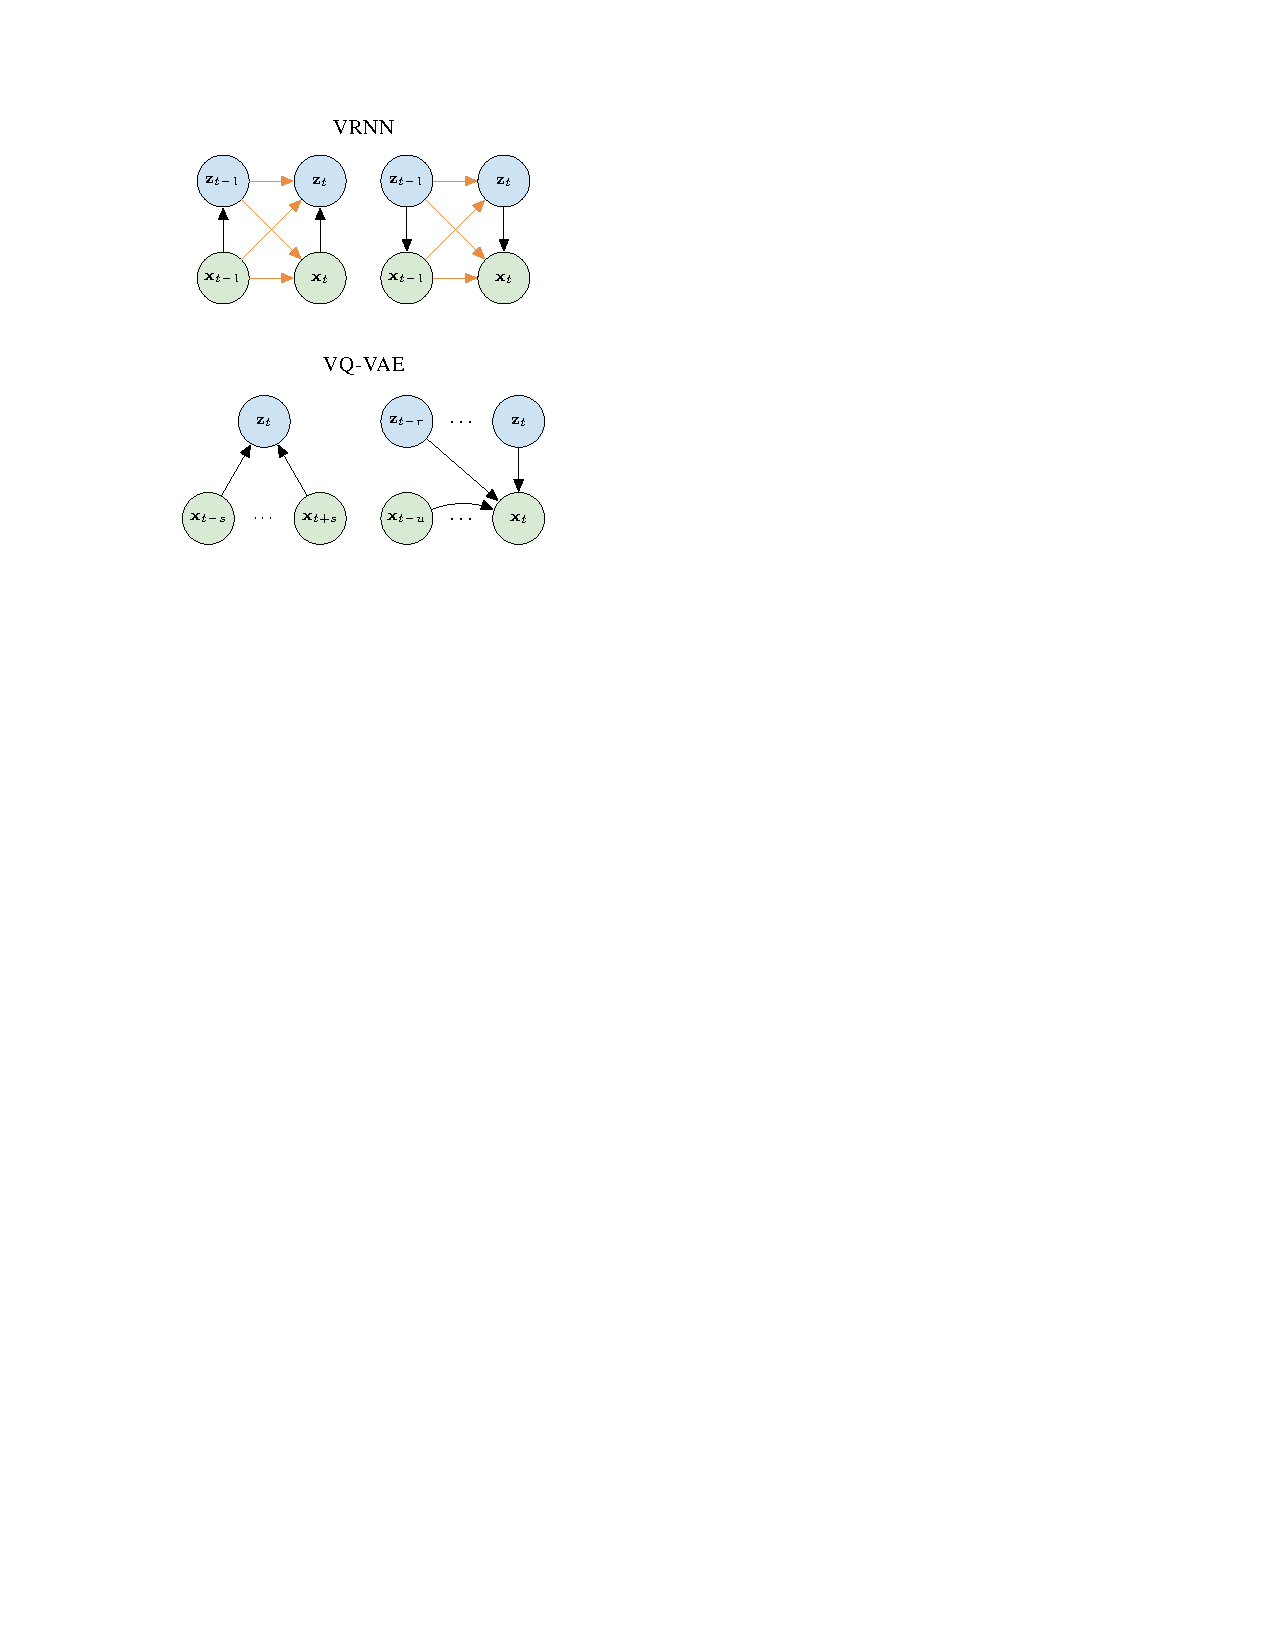
\includegraphics[width=0.8\textwidth]{figures/brief-vrnn-vqvae.pdf}
            \end{figure}
        \end{column}

        \begin{column}{0.5\textwidth}
            \begin{figure}
                \centering
                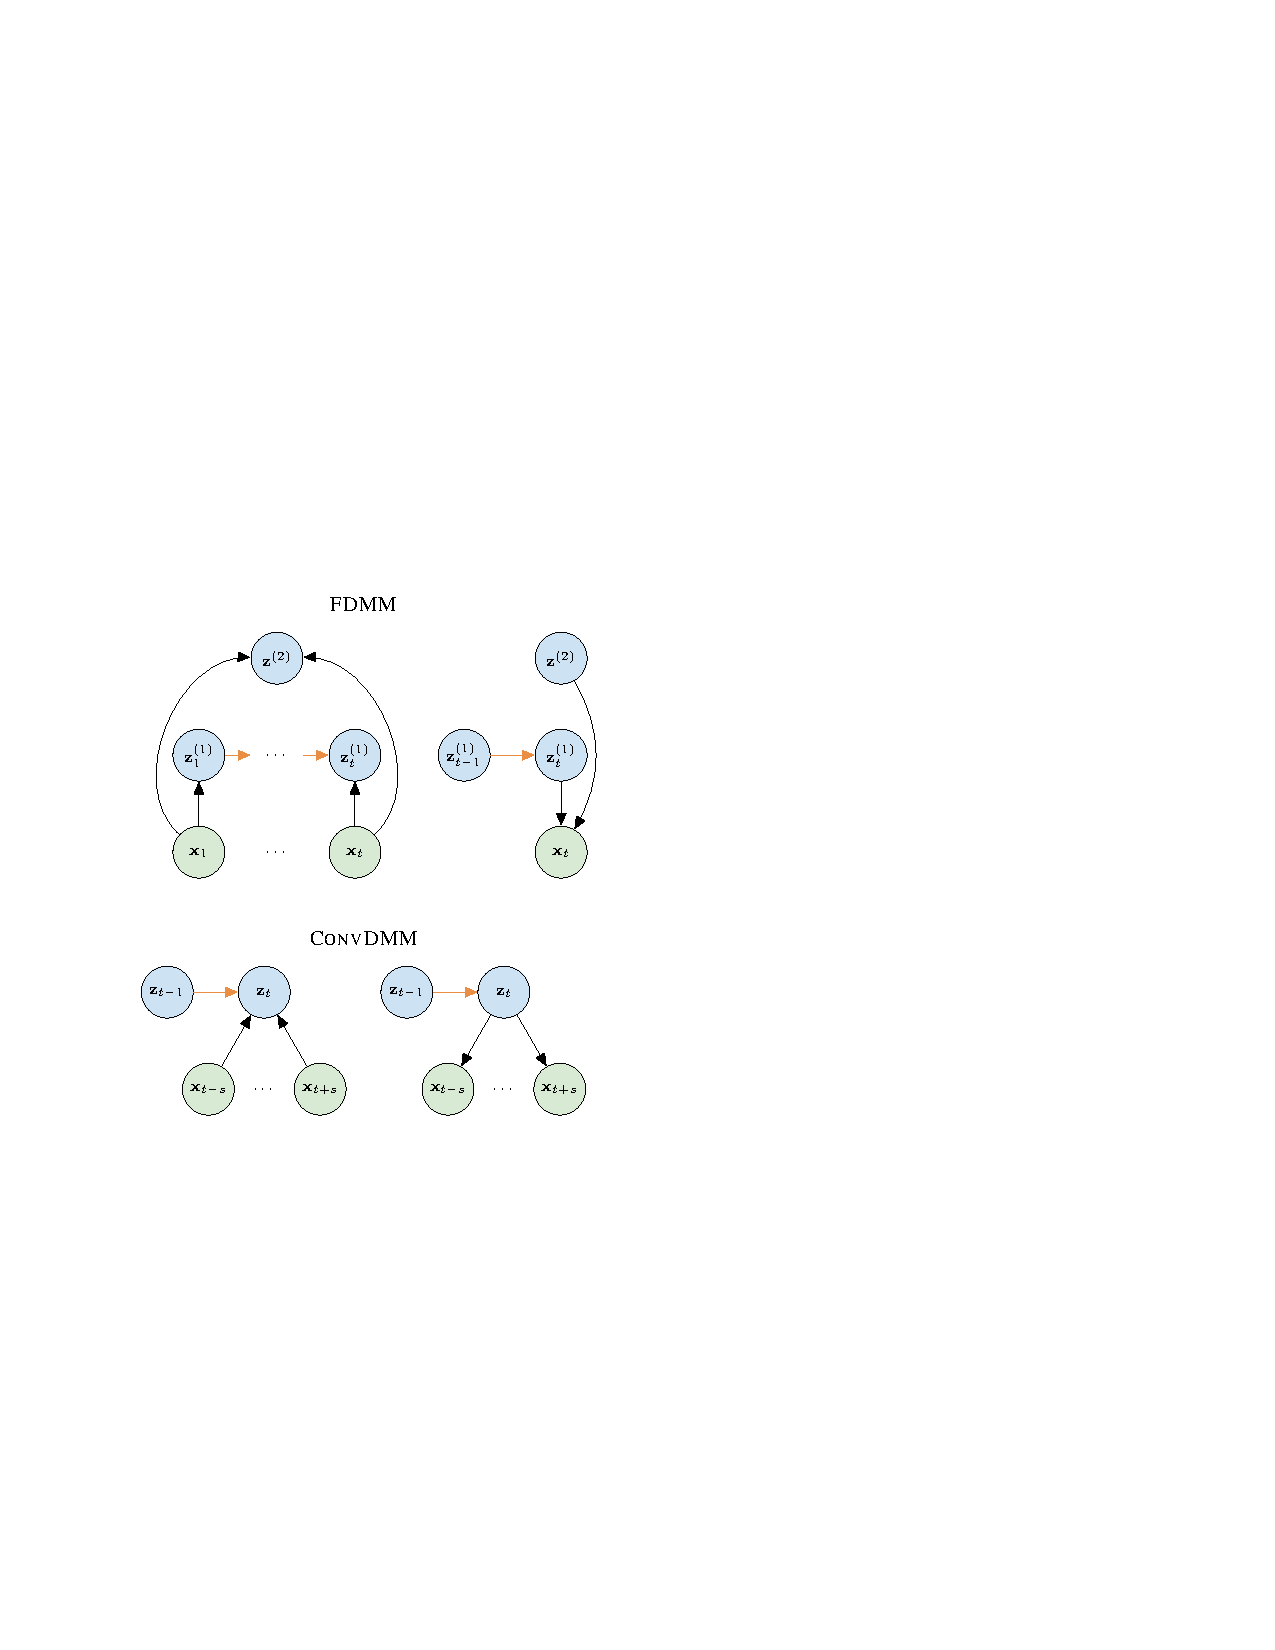
\includegraphics[width=0.8\textwidth]{figures/brief-fdmm-convdmm.pdf}
            \end{figure}            
        \end{column}

    \end{columns}

    \definecolor{sharedcolor}{RGB}{234 142 67} % mørk orange
    \blfootnote{\scalebox{0.6}{{\color{sharedcolor} Orange edges} indicate parameters shared between inference and generative models.}}
\end{frame}


\begin{frame}
    \frametitle{Overview of LVM probabilistic components}

    \begin{table}
        % \caption[A comprehensive overview of observation, prior and inference models for VAE type latent variable models with a single latent variable.]{ A comprehensive overview of observation, prior and inference models for VAE type latent variable models with a single latent variable. The observation, prior and inference models may all belong to one or more of the categories listed under them as detailed in \cref{sec:plvms}. The types listed here serve as primitives from which more complex structures can be constructed including models with hierarchies of multiple latent variables.}
        % \label{tab:lvm-model-primitives}
        % \begin{center}
        \centering
        % \renewcommand{\arraystretch}{1.1}
        \resizebox{0.8\textheight}{!}{%
            \begin{tabular}{ l l l } 
                \toprule
                \multicolumn{2}{l}{\textbf{\textsc{Type}}} & \textbf{\textsc{Form}} \\
                \midrule
                \multicolumn{3}{c}{\textsc{Observation model}} \\
                \midrule
                \textbf{\textsc{arx}} & Autoregressive on $\mathbf{x}_t$      & $p(\mathbf{x}_t|\mathbf{x}_{1:t-1})$ \\
                \textbf{\textsc{loc}} & Local latent variable                 & $p(\mathbf{x}_{t}|\mathbf{z}_{1:t})$ \\
                \textbf{\textsc{glb}} & Global latent variable                & $p(\mathbf{x}_{t}|\mathbf{z})$ \\
                \midrule
                \multicolumn{3}{c}{\textsc{Prior}} \\
                \midrule
                \textbf{\textsc{arx}} & Autoregressive on $\mathbf{x}_t$      & $p(\mathbf{z}_t|\mathbf{x}_{1:t-1})$ \\
                \textbf{\textsc{arz}} & Autoregressive on $\mathbf{z}_t$      & $p(\mathbf{z}_t|\mathbf{z}_{1:t-1})$ \\
                \textbf{\textsc{ind}} & Locally independent $\mathbf{z}_t$                 & $p(\mathbf{z}_t)$ \\
                \textbf{\textsc{glb}} & Global latent variable                & $p(\mathbf{z})$ \\
                \midrule
                \multicolumn{3}{c}{\textsc{Inference model}} \\
                \midrule
                \textbf{\textsc{arz}} & Autoregressive on $\mathbf{z}_t$      & $q(\mathbf{z}_t|\mathbf{z}_{1:t-1})$ \\
                \textbf{\textsc{flt}} & Filtering                             & $q(\mathbf{z}_t|\mathbf{x}_{1:t})$ \\
                \textbf{\textsc{lsm}} & Local smoothing                       & $q(\mathbf{z}_t|\mathbf{x}_{t-r:t+r})$ \\
                \textbf{\textsc{gsm}} & Global smoothing                      & $q(\mathbf{z}_t|\mathbf{x}_{1:T})$ \\
                \textbf{\textsc{glb}} & Global latent variable                & $q(\mathbf{z}|\mathbf{x}_{1:T})$ \\
                \bottomrule
            \end{tabular}
        }
        % \end{center}
    \end{table}

\end{frame}


\begin{frame}
    \frametitle{Classification of selected LVMs for speech}

    \begin{table}
        % \caption[Classification of selected latent variable models.]{ Selected latent variable models classified according the attributes defined throughout \cref{sec:plvms}. See \cref{tab:lvm-model-primitives} for the probability distributions that correspond to each of the attribute short-hands. \textbf{\textsc{hie}} indicates a hierarchical representation.}
        % \label{tab:lvm-taxonomy}
        % \begin{center}
        \centering
        \setlength{\tabcolsep}{3pt}
        \renewcommand{\arraystretch}{1.1}
        \resizebox{0.7\textwidth}{!}{%
            \begin{tabular}{ l | c c c | c c c c | c c c c c | c } 
                \toprule
                \multicolumn{2}{c}{} & 
                \multicolumn{3}{c}{\textsc{Observation}} & 
                \multicolumn{4}{c}{\textsc{Prior}} & 
                \multicolumn{5}{c}{\textsc{Inference}} \\
                \textbf{\textsc{model}} & 
                \textbf{\textsc{arx}} & 
                \textbf{\textsc{loc}} & 
                \textbf{\textsc{glb}} &  
                \textbf{\textsc{arx}} & 
                \textbf{\textsc{arz}} & 
                \textbf{\textsc{ind}} & 
                \textbf{\textsc{glb}} &  
                \textbf{\textsc{arz}} & 
                \textbf{\textsc{flt}} & 
                \textbf{\textsc{lsm}} & 
                \textbf{\textsc{gsm}} & 
                \textbf{\textsc{glb}} &
                \textbf{\textsc{hie}} \\
                \midrule
                %                                                              OBSERVATION       |              PRIOR                |                  INFERENCE       
                %                                                         ARX      LOC      GLB      ARX      ARZ     IND      GLB      ARZ      FLT      LSM      GSM      GLB
                \textbf{VRNN} \footnotesize{\parencite{chung_recurrent_2015}}          & \cmark & \cmark & \xmark & \cmark & \cmark & \xmark & \xmark & \cmark & \cmark & \xmark & \xmark & \xmark & \xmark \\
                \textbf{SRNN} \footnotesize{\parencite{fraccaro_sequential_2016}}      & \cmark & \cmark & \xmark & \cmark & \cmark & \xmark & \xmark & \cmark & \xmark & \xmark & \cmark & \xmark & \xmark \\
                \textbf{HMM-VAE} \footnotesize{\parencite{ebbers_hidden_2017}}         & \xmark & \cmark & \xmark & \xmark & \cmark & \xmark & \xmark & \cmark & \cmark & \xmark & \xmark & \xmark & \cmark \\
                \textbf{ConvVAE} \footnotesize{\parencite{hsu_learning_2017}}          & \xmark & \xmark & \cmark & \xmark & \xmark & \xmark & \cmark & \xmark & \xmark & \xmark & \cmark & \cmark & \xmark \\
                \textbf{FHVAE} \footnotesize{\parencite{hsu_unsupervised_2017}}        & \xmark & \cmark & \cmark & \xmark & \xmark & \cmark & \cmark & \xmark & \xmark & \xmark & \cmark & \cmark & \cmark \\
                \textbf{VQ-VAE} \footnotesize{\parencite{oord_neural_2018}}            & \cmark & \cmark & \xmark & \xmark & \xmark & \cmark & \xmark & \xmark & \xmark & \cmark & \xmark & \xmark & \xmark \\
                \textbf{BHMM-VAE} \footnotesize{\parencite{glarner_full_2018}}         & \xmark & \cmark & \xmark & \xmark & \cmark & \xmark & \xmark & \cmark & \cmark & \xmark & \xmark & \xmark & \xmark \\
                \textbf{STCN} \footnotesize{\parencite{aksan_stcn_2019}}               & \xmark & \cmark & \xmark & \cmark & \xmark & \xmark & \xmark & \xmark & \cmark & \xmark & \xmark & \xmark & \cmark \\
                \textbf{FDMM} \footnotesize{\parencite{khurana_factorial_2019}}        & \xmark & \cmark & \cmark & \xmark & \cmark & \xmark & \cmark & \cmark & \cmark & \xmark & \xmark & \cmark & \cmark \\
                \textbf{ConvDMM} \footnotesize{\parencite{khurana_convolutional_2020}} & \xmark & \cmark & \xmark & \xmark & \cmark & \xmark & \xmark & \cmark & \xmark & \cmark & \xmark & \xmark & \xmark \\
                \bottomrule
            \end{tabular}
        }
        % \end{center}
    \end{table}

\end{frame}

\begin{frame}
    \frametitle{Comparison of LVMs and SSL methods}

    \begin{table}
        % \caption[Classification of selected self"=supervised and probabilistic latent variable models.]{ Selected models classified according to the binary attributes identified throughout the text. The models are sorted according to first publication date on arXiv which might differ from the citation year. \textbf{\textsc{msk}}: masking, \textbf{\textsc{prd}}: prediction, \textbf{\textsc{con}}: contrastive, \textbf{\textsc{rec}}: reconstruction, \textbf{\textsc{qtz}}: quantization, \textbf{\textsc{gen}}: generative, \textbf{\textsc{frz}}: frozen, \textbf{\textsc{ftn}}: fine"=tuned, \textbf{\textsc{loc}}: local, \textbf{\textsc{glo}}: global.}
        % \label{tab:model-taxonomy}
        % \begin{center}
        \centering
        \setlength{\tabcolsep}{3pt}
        \renewcommand{\arraystretch}{1.1}
        \resizebox{1\textheight}{!}{%
            \begin{tabular}{ l l | c c c c c c | c c c | c c } 
                \toprule
                
                \multicolumn{2}{c}{} & 
                \multicolumn{6}{c}{\textsc{model and task design}} & 
                \multicolumn{3}{c}{\textsc{resolution}} &
                \multicolumn{2}{c}{\makebox[0pt][c]{\textsc{usage}}} \\
                & \textbf{\textsc{model}} &
                \textbf{\textsc{msk}} & 
                \textbf{\textsc{prd}} & 
                \textbf{\textsc{con}} &  
                \textbf{\textsc{rec}} &  
                \textbf{\textsc{qtz}} & 
                \textbf{\textsc{gen}} & 
                \textbf{\textsc{loc}} & 
                \textbf{\textsc{glb}} & 
                \textbf{\textsc{var}} & 
                \textbf{\textsc{frz}} & 
                \textbf{\textsc{ftn}} \\
                
                \midrule
                % \multicolumn{11}{c}{\textsc{Self-supervised models}} \\
                % \midrule
                %                                                           MSK      PRD      CON      REC      QTZ      GEN      LOC      GLB     VAR      FRZ      FTN
                \verticalmultirow{9}{\textsc{Self-supervised models}} 
                % & \textbf{Audio Word2vec} \footnotesize{\parencite{chung_audio_2016}}      & \cmark & \xmark & \xmark & \cmark & \xmark & \xmark & \xmark & \cmark & \xmark & \cmark & \xmark \\
                % & \textbf{Speech2Vec} \footnotesize{\parencite{chung_speech2vec_2018}}     & \xmark & \cmark & \xmark & \cmark & \xmark & \xmark & \xmark & \cmark & \xmark & \cmark & \xmark \\
                % & \textbf{Unspeech} \footnotesize{\parencite{milde_unspeech_2018}}         & \xmark & \cmark & \cmark & \xmark & \xmark & \xmark & \xmark & \cmark & \xmark & \cmark & \xmark \\
                
                & \textbf{CPC} \footnotesize{\parencite{oord_representation_2018}}         & \xmark & \cmark & \cmark & \xmark & \xmark & \xmark & \cmark & \xmark & \xmark & \cmark & \xmark \\
                
                & \textbf{APC} \footnotesize{\parencite{chung_unsupervised_2019}}          & \xmark & \cmark & \xmark & \cmark & \xmark & \xmark & \cmark & \xmark & \xmark & \cmark & \xmark \\ % 5/4
                & \textbf{wav2vec} \footnotesize{\parencite{schneider_wav2vec_2019}}       & \xmark & \cmark & \cmark & \xmark & \xmark & \xmark & \cmark & \xmark & \xmark & \cmark & \xmark \\ % 11/4
                & \textbf{Mockingjay}  \footnotesize{\parencite{liu_mockingjay_2020}}      & \cmark & \xmark & \xmark & \cmark & \xmark & \xmark & \cmark & \xmark & \xmark & \cmark & \cmark \\ % 25/10-19
                & \textbf{wav2vec 2.0} \footnotesize{\parencite{baevski_wav2vec_2020}}     & \cmark & \xmark & \cmark & \xmark & \cmark & \xmark & \cmark & \xmark & \xmark & \xmark & \cmark \\ % 20/6
                & \textbf{NPC} \footnotesize{\parencite{liu_nonautoregressive_2020}}       & \cmark & \xmark & \xmark & \cmark & \cmark & \xmark & \cmark & \xmark & \xmark & \cmark & \xmark \\ % 1/11
                & \textbf{DeCoAR 2.0} \footnotesize{\parencite{ling_decoar_2020}}          & \cmark & \xmark & \xmark & \cmark & \cmark & \xmark & \cmark & \xmark & \xmark & \cmark & \xmark \\ % 11/12
                % & \textbf{SCPC} \footnotesize{\parencite{bhati_segmental_2021}}            & \xmark & \cmark & \cmark & \xmark & \xmark & \xmark & \cmark & \xmark & \cmark & \cmark & \xmark \\ % 3/6
                & \textbf{HuBERT} \footnotesize{\parencite{hsu_hubert_2021}}               & \cmark & \xmark & \xmark & \xmark & \cmark & \xmark & \cmark & \xmark & \xmark & \xmark & \cmark \\ % 14/6
                & \textbf{data2vec} \footnotesize{\parencite{baevski_data2vec_2022}}       & \cmark & \xmark & \xmark & \xmark & \xmark & \xmark & \cmark & \xmark & \xmark & \xmark & \cmark \\ % 16/6

                \midrule
                % \multicolumn{11}{c}{\textsc{Probabilistic latent variable models}} \\
                % \midrule
                %                                                           MSK      PRD      CON      REC      QTZ      GEN      LOC      GLO     VAR      FRZ      FTN
                \verticalmultirow{8}{\textsc{Latent variable models}}
                & \textbf{VRNN} \footnotesize{\parencite{chung_recurrent_2015}}          & \xmark & \xmark & \xmark & \cmark & \xmark & \cmark & \cmark & \xmark & \xmark & \cmark & \xmark \\
                & \textbf{SRNN} \footnotesize{\parencite{fraccaro_sequential_2016}}      &\xmark & \xmark & \xmark & \cmark & \xmark & \cmark & \cmark & \xmark & \xmark & \cmark & \xmark \\
                % & \textbf{HMM-VAE} \footnotesize{\parencite{ebbers_hidden_2017}}         & \xmark & \xmark & \xmark & \cmark & \xmark & \cmark & \cmark & \xmark & \xmark & \cmark & \xmark \\
                & \textbf{ConvVAE} \footnotesize{\parencite{hsu_learning_2017}}          & \xmark & \xmark & \xmark & \cmark & \xmark & \cmark & \xmark & \cmark & \xmark & \cmark & \xmark \\
                & \textbf{FHVAE} \footnotesize{\parencite{hsu_unsupervised_2017}}        & \xmark & \xmark & \xmark & \cmark & \xmark & \cmark & \cmark & \cmark & \xmark & \cmark & \xmark \\
                & \textbf{VQ-VAE} \footnotesize{\parencite{oord_neural_2018}}            & \xmark & \xmark & \xmark & \cmark & \cmark & \cmark & \cmark & \xmark & \xmark & \cmark & \xmark \\
                % & \textbf{BHMM-VAE} \footnotesize{\parencite{glarner_full_2018}}         & \xmark & \xmark & \xmark & \cmark & \xmark & \cmark & \cmark & \xmark & \xmark & \cmark & \xmark \\
                & \textbf{STCN} \footnotesize{\parencite{aksan_stcn_2019}}               & \xmark & \xmark & \xmark & \cmark & \xmark & \cmark & \cmark & \xmark & \xmark & \cmark & \xmark \\
                & \textbf{FDMM} \footnotesize{\parencite{khurana_factorial_2019}}        & \xmark & \xmark & \xmark & \cmark & \xmark & \cmark & \cmark & \cmark & \xmark & \cmark & \xmark \\
                & \textbf{ConvDMM} \footnotesize{\parencite{khurana_convolutional_2020}} & \xmark & \xmark & \xmark & \cmark & \xmark & \cmark & \cmark & \xmark & \xmark & \cmark & \xmark \\
                \bottomrule
            \end{tabular}
        }
        % \end{center}
    \end{table}

\end{frame}


% ======================================================================================================================




\end{document}